\documentclass[msc,numbers]{coppe}
\usepackage[utf8]{inputenc}
\usepackage{amsmath,amssymb}
\usepackage{hyperref}
\usepackage{todonotes}
\usepackage{booktabs}
\usepackage{graphicx}
\usepackage{subcaption}
\usepackage{lipsum}
\usepackage{tcolorbox}
\usepackage[inline]{enumitem}

\makelosymbols
\makeloabbreviations

\DeclareMathOperator{\atantwo}{atan2}

\begin{document}
  \title{Avaliação da dinâmica de manipuladores robóticos sobre bases flexíveis}
  \foreigntitle{Analysis of the dynamics of robotic manipulators on flexible
  basis}
  \author{Estevão}{Fróes Ferrão}
  \advisor{Prof.}{Fernando}{ Augusto de Noronha Castro Pinto}{D.Sc.}
  %\advisor{Prof.}{Nome do Segundo Orientador}{Sobrenome}{Ph.D.}
  %\advisor{Prof.}{Nome do Terceiro Orientador}{Sobrenome}{D.Sc.}

  \examiner{Prof.}{Nome do Primeiro Examinador Sobrenome}{D.Sc.}
  \examiner{Prof.}{Nome do Segundo Examinador Sobrenome}{Ph.D.}
  \examiner{Prof.}{Nome do Terceiro Examinador Sobrenome}{D.Sc.}
  \examiner{Prof.}{Nome do Quarto Examinador Sobrenome}{Ph.D.}
  \examiner{Prof.}{Nome do Quinto Examinador Sobrenome}{Ph.D.}
  \department{PEM}
  \date{03}{2018}

  \keyword{dinâmica multicorpos}
  \keyword{modelagem cinemática}
  \keyword{análise modal}
  \keyword{robótica de serviço}
  \keyword{erros de trajetória}

  \maketitle

  \frontmatter
  \dedication{A algu\'em cujo valor \'e digno desta dedicat\'oria.}


  \chapter*{Agradecimentos}

Gostaria de agradecer a todos.

  \begin{abstract}

Apresenta-se, nesta tese, ...

\end{abstract}


  \begin{foreignabstract}

In this work, we present ...

\end{foreignabstract}


  \tableofcontents
  \listoffigures
  \listoftables
  \printlosymbols
  \printloabbreviations

  \mainmatter
  \chapter{Introdução}

% Segundo a norma de formata{\c c}\~ao de teses e disserta{\c c}\~oes do
% Instituto Alberto Luiz Coimbra de P\'os-gradua{\c c}\~ao e Pesquisa de
% Engenharia (COPPE), toda abreviatura deve ser definida antes de
% utilizada.\abbrev{COPPE}{Instituto Alberto Luiz Coimbra de P\'os-gradua{\c
% c}\~ao e Pesquisa de Engenharia}
% 
% Do mesmo modo, \'e imprescind\'ivel definir os s\'imbolos, tal como o
% conjunto dos n\'umeros reais $\mathbb{R}$ e o conjunto vazio $\emptyset$.
% \symbl{$\mathbb{R}$}{Conjunto dos n\'umeros reais}
% \symbl{$\emptyset$}{Conjunto vazio}

% -.~.-.~.-.~.-.~.-.~.-.~.-.~.-.~.-.~.-.~.-.~.-
\section{Motivação}

Com uma população de robôs industriais cada vez maior em diversas áreas de
automação, surgem também novas ideias e aplicações. Seja para melhoria da
eficiência, impossibilidade de realização humana ou tarefas em ambientes hostis,
utilizar robôs se torna uma alternativa atrativa também para trabalhos
\textit{in situ}, ou operacional em campo, locais não planejados originalmente
para a aplicação robótica.
Ambientes bem estruturados são geralmente um requisito da maioria das aplicações
utilizando manipuladores robóticos, que não têm capacidade para lidar com ações
ou efeitos do ambiente e, caso ocorram, não pode-se garantir a segurança ou
qualidade da tarefa a ser executada.

Um exemplo de aplicação robótica \textit{in situ} é o sistema de manutenção de
pás de turbinas, denominado EMMA\cite{freitas2017state}.
É um projeto desenvolvido pela empresa THIRTEEN ROBOTICS em parceria com o
LEAD/COPPE-UFRJ e a Energia Sustentável do Brasil (ESBR). Este sistema consiste
em realizar um procedimento de manutenção do revestimento das pás de turbinas do
tipo Kaplan em usinas hidrelétricas, que sofrem desgaste por abrasão e
cavitação, perdendo sua camada de proteção devendo ser reaplicada. Atualmente,
as pás são desmontadas e levadas para um galpão em que, num ambiente bem
estruturado, um robô de grande porte reaplica o revestimento.
O objetivo do projeto EMMA é poupar todo o procedimento de desmontagem e
transporte destas pás, que geram um alto custo e tempo, por um sistema de
revestimento robótico \textit{in situ}, ou seja, dentro do ambiente da turbina.

O desafio deste projeto está em conseguir instalar o robô com segurança e
praticidade, no ambiente confinado e de difícil acesso da unidade geradora. Por
conta do único acesso ser através de uma escotilha de $850~mm$ de diâmetro, o
robô deve ser de médio a pequeno porte, ter uma base para sua fixação e
posicionamento próximo a pá, que seja leve e modular, para fácil transporte,
montagem e acesso pela escotilha. O desafio torna-se ainda maior se considerado
que o processo de revestimento tem requisitos que devem ser controlados com
precisão, para garantir sua qualidade. Este tipo de revestimento só pode ser
aplicado roboticamente porque desvios de posição, orientação ou velocidade do
processo, podem simplesmente reprovar ou inviabilizar o procedimento.

Por isso, considerando todas as restrições do sistema, projetou-se para a
solução \textit{in situ}, uma base metálica, leve e modular, que possibilitasse
o posicionamento do robô próximo às pás, em diversas configurações de montagem.
Porém, simulações estáticas de carregamento, realizadas por Anáise por Elementos
Finitos apresentaram resultados que o comportamento dinâmico da estrutura,
poderia causar grandes amplitudes de deslocamento.
Neste momento percebeu-se a necessidade de ter um modelo capaz de simular a
tarefa de revestimento e obter-se assim o comportamento dinâmico acoplado entre
base e robô, para então quantificar os desvios causados aos parâmetros
controlados do processo de revestimento.

A busca por linhas de pesquisa sobre robôs em bases flexíveis revelou que o tema
foi explorado principalmente sob um ponto de vista de manipuladores macro-micro,
sistemas em que consideram a flexibilidade do manipulador, e de métodos de
controle ativos para amortecer as vibrações. Nestes estudos, carece uma
metodologia mais sistemática para avaliação dos efeitos da rigidez e
amortecimento da base, e sua relação com a geometria e materiais da estrutura.
Assim como, dos erros em relação aos parâmetros controlados de determinado
processo, causados pela dinâmica da base. Esta pesquisa tem como motivação aliar
o método de avaliação do sistema robô-base a aplicações práticas da indústria,
tendo como principal estudo de caso o sistema de revestimento robótico do
projeto EMMA.

De modo geral, pode-se afirmar que a ação do robô ao realizar
determinada tarefa irá originar, por reação, deslocamentos dinâmicos em sua
base. Estes deslocamentos causarão algum impacto na tarefa a ser realizada como:
mudanças de orientação, velocidade e posicionamento da ferramenta acoplada ao
manipulador. Estes efeitos não são considerados nos métodos de controle
convencionais das juntas do manipulador, porque não podem ser previstos sem que
haja alguma instrumentação periférica, capaz de medir e enviar tais informações
ao controlador.

Caso a base não ofereça a rigidez necessária, a amplitude dos deslocamentos pode
simplesmente inviabilizar a tarefa desejada e, se possível, modificações na
estrutura da base ou uma nova estrutura devem ser projetadas. Por isso, ser
capaz de estimar o comportamento do sistema, por simulação no computador, é uma
importante ferramenta, que pode principalmente evitar o projeto e fabricação de
uma solução equivocada.


% O amortecimento da estrutura que serve de base para o manipulador tem um papel
% importante na dinâmica do sistema. Como foi demonstrado, o modelo MBS
% acoplado robô-base requer como entrada os parâmetros de inércia, rigidez e amortecimento
% da base. Os dados de inércia são facilmente obtidos pelo modelo CAD e a matriz
% de inércia pela Análise por Elementos Finitos. Entretanto, estas
% ferramentas não são capazes de fornecer informações sobre o amortecimento.
% Modelar o amortecimento é um problema constante na engenharia de sistemas
% mecânicos e continua um desafio.
% 
% O sistema robô-base não possui nenhum elemento com a finalidade específica de
% controle ou absorção de vibrações. O que ocorre é o citado amortecimento
% estrutural (seção~\ref{sec::amortecimento}), formado principalmente pelo
% amortecimento do material \todo{Inlcuir referência no texto} e por atrito,
% devido a folgas nos elementos de conexão, parafusos por exemplo.
% 
% Apesar de existir métodos para estimar o amortecimento material e de atrito
% analiticamente, estes são adequados para estruturas muito simples e uniformes,
% como vigas, placas ou corpos de prova. A estrutura que forma a base do robô é
% relativamente muito complexa, possuindo diferentes materiais, conexões e formas,
% o que torna impossível modelar analiticamente o amortecimento.
% 
% Logo, recorre-se ao método experimental para obter o amortecimento da base.
% A vantagem é que por este método, obtém-se os parâmetros do comportamento total
% da estrutura, não importando as infinitas interações internas dos materiais e de
% atrito impossíveis de se medir ou quantificar individualmente.
% Mais especificamente, o que importará mesmo é o comportamento do ponto de
% interação robô-base.

% O objetivo do projeto desta plataforma não era o de oferecer grande
% flexibilidade, mas pelo contrário, ser suficientemente rígida para operar o robô
% com segurança durante testes do projeto EMMA. A análise deste modelo de base
% será interessante para comparar com o modelo rígido e verificar se o projeto,
% que foi realizado antes de existir o método proposto neste trabalho,
% atende a este requisito.


% -.~.-.~.-.~.-.~.-.~.-.~.-.~.-.~.-.~.-.~.-.~.-
\section{Objetivos}

Este trabalho tem como objetivo oferecer um método para calcular e quantificar
os deslocamentos teóricos da base, quando excitada pelo movimento do manipulador
robótico, e assim calcular os erros de posicionamento, velocidade e orientação
no efetuador do robô, ao longo de uma trajetória. 

Também oferece uma forma de avaliar o efeito, no resultado da trajetória, de
alterações estruturais na base. Se resultarem erros fora de uma margem de
tolerância admitida, o método pode ser utlizado iterativamente, realizando-se
modificações estratégicas da base -- como materiais, configuração geométrica,
apoios, reforço estrutural, massa, etc.
O objetivo deste processo é, em um ambiente de simulação, verificar a nova base,
e a partir dos resultados fazer as modificações até atingir a tolerância que
satisfaz a qualidade da tarefa.

Por fim, tem-se por objetivo discutir estratégias futuras de instrumentação e
controle, para levar em consideração as perturbações causadas pela base e
corrigir as diferenças de posicionamento, velocidade e orientação das juntas do
manipulador.


% -.~.-.~.-.~.-.~.-.~.-.~.-.~.-.~.-.~.-.~.-.~.-
\section{Ferramentas utilizadas}

De maneira geral, o repertório de programas utilizados compõe um conjunto de
ferramentas importantes para o método, como: Álgebra Computacional Simbólica
(CAS), Análise por Elementos Finitos (AEF), Desenho Assistido por Computador
(CAD), aquisição e tratamento de dados experimentais. Esta pesquisa também tem
como preocupação permitir ao usuário utilizar as ferramentas que estiverem à sua
disposição pessoal ou da instituição (laboratório, empresa, universidade, etc.),
não limitando ao uso de qualquer \textit{software} em especial. Embora tenham
sido utilizados programas de alto nível ficará claro que outros também poderiam
ter sido utilizados. Por isso, são listados a seguir os programas escolhidos e
também alternativas disponíveis no mercado.

\subsubsection{Sophia-Maple}

Sophia é um conjunto de rotinas, desenvolvido por \citet{lesser1995analysis}
para modelar sistemas mecânicos multicorpos e derivar suas equações de
movimento. Foi criado originalmente para Maple, depois foi adaptada uma uma
versão para o Mathematica.
Maple\cite{maple} é um programa de álgebra simbólica computacional (CAS), com
ênfase em manipulações algébricas simbólicas ao invés de numéricas, o que
permite modelar e solucionar sistemas dinâmicos simbolicamente. O pacote Sophia,
utilizado com o Maple será descrito apenas por Sophia-Maple.

Alternativas:
%
\begin{enumerate*}
	\item Mathematica;
	\item SymPy;
\end{enumerate*}

\subsubsection{SolidWorks}

SolidWorks\cite{solidworks} é um programa de CAD 3D, utilizado principalmente
para modelagem de peças e conjuntos mecânicos.
Este programa tem interface amigável que facilita o desenho de conjuntos e
montagens complexas. Permite também a definição do material de cada peça, por
fornecer vasta lista de materiais e suas propriedades físicas e mecânicas.
Realiza automaticamente o cálculo, por exemplo, de massa, centro de
gravidade, momentos de inércia e propriedades de seção transversal, que são
muito úteis para o método. Também permite a conversão do modelo 3D para diversos
formatos CAD, que facilitam a exportação de versões para Análise por Elementos
Finitos para outros programas.

Alternativas:
%
\begin{enumerate*}
	\item AutoCAD;
	\item CATIA;
	\item Pro/ENGINEER.
\end{enumerate*}

\subsubsection{Simulation Mechanical}

O Simulation Mechanical\cite{autodesk} é um programa para Análise por Elementos
Finitos distribuido pela Autodesk.  Realiza análises estáticas lineares e não-lineares,
análise modal, análise de carregamento transiente, análises térmicas e de
mecânica dos fluidos.
É utilizado nesta pesquisa para simulações de carregamento estático linear, a
fim de determinar a matriz de rigidez da base do manipulador. O programa permite
grande variedade de formatos para importação de modelos CAD, o que facilita a
integração com o SolidWorks.

Alternativas:
%
\begin{enumerate*}
	\item Abaqus;
	\item Ansys;
	\item SolidWorks Simulation.
\end{enumerate*}


\subsubsection{SignalExpress e ME`Scope VES}

Para determinação de parâmetros modais da base do robô é necessário obter dados
experimentais através de instrumentação da base. São utilizados 2 programas: o
primeiro para aquisição, visualização e tratamento dos dados; o segundo para
cálculo dos parâmetros modais.

SignalExpress\cite{signalexpress} é programa aquisição, análise e
apresentação de dados compatível com diversos instrumentos e sistemas de
aquisição e medição experimentais e operacionais. 
É utilizado nesta pesquisa para adquirir e processar os dados do ensaio
experimental de uma versão de testes da base do robô.

O ME'Scope VES (\textit{Visual Engineering Series})\cite{mescope} é um programa
para facilitar a visualização e análise de vibrações de máquinas e estruturas
mecânicas, utilizando os dados reais registrados experimentalmente. O programa
também realiza análise modal, a partir das Funções de Resposta em Frequência
(FRF's) dos dados importados. É utilizado portanto para  determinar o
amortecimento modal, parâmetro necessário ao modelo teórico da base.

Alternativas:
%
\begin{enumerate*}
	\item Brüel \& Kjær PULSE;
	\item OROS Modal Analysis;
	\item LabVIEW.
\end{enumerate*}

\section{Notação}

% Texto introdutório considerando a pluralidade de referências.

  \chapter{Revisão Bibliográfica}

% Para ilustrar a completa ades\~ao ao estilo de cita{\c c}\~oes e listagem de
% refer\^encias bibliogr\'aficas, a Tabela~\ref{tab:citation} apresenta cita{\c
% c}\~oes de alguns dos trabalhos contidos na norma fornecida pela CPGP da
% COPPE, utilizando o estilo num\'erico.
% 
% \begin{table}[h]
% \caption{Exemplos de cita{\c c}\~oes utilizando o comando padr\~ao
%   \texttt{\textbackslash cite} do \LaTeX\ e
%   o comando \texttt{\textbackslash citet},
%   fornecido pelo pacote \texttt{natbib}.}
% \label{tab:citation}
% \centering
% {\footnotesize
% \begin{tabular}{|c|c|c|}
%   \hline
%   Tipo da Publica{\c c}\~ao & \verb|\cite| & \verb|\citet|\\
%   \hline
%   Livro & \cite{book-example} & \citet{book-example}\\
%   Artigo & \cite{article-example} & \citet{article-example}\\
%   Relat\'orio & \cite{techreport-example} & \citet{techreport-example}\\
%   Relat\'orio & \cite{techreport-exampleIn} & \citet{techreport-exampleIn}\\
%   Anais de Congresso & \cite{inproceedings-example} &
%     \citet{inproceedings-example}\\
%   S\'eries & \cite{incollection-example} & \citet{incollection-example}\\
%   Em Livro & \cite{inbook-example} & \citet{inbook-example}\\
%   Disserta{\c c}\~ao de mestrado & \cite{mastersthesis-example} &
%     \citet{mastersthesis-example}\\
%   Tese de doutorado & \cite{phdthesis-example} & \citet{phdthesis-example}\\
%   \hline
% \end{tabular}}
% \end{table}

% -.~.-.~.-.~.-.~.-.~.-.~.-.~.-.~.-.~.-.~.-.~.-
\section{Manipuladores robóticos industriais}


% -.~.-.~.-.~.-.~.-.~.-.~.-.~.-.~.-.~.-.~.-.~.-
\section{Tarefas de precisão utilizando manipuladores robóticos}

\subsection{Sistema de revestimento por asperção térmica}

\subsection{Tarefas robóticas \textit{in-situ}}


% -.~.-.~.-.~.-.~.-.~.-.~.-.~.-.~.-.~.-.~.-.~.-
\section{Manipuladores flexíveis}


% -.~.-.~.-.~.-.~.-.~.-.~.-.~.-.~.-.~.-.~.-.~.-
\section{Manipuladores sobre bases flexíveis}


% -.~.-.~.-.~.-.~.-.~.-.~.-.~.-.~.-.~.-.~.-.~.-
\section{Dinâmica de Sistemas Multicorpos (MBS)}

\subsection{Cinemática}

\subsection{Dinâmica}

\subsection{Cinemática Inversa e planejamento de trajetória}

\subsection{Equações de Movimento}

\subsection{Sophia-Maple e Método de Kane}


% -.~.-.~.-.~.-.~.-.~.-.~.-.~.-.~.-.~.-.~.-.~.-
\section{Análise modal em estruturas}

\subsection{Frequência Natural, Modo de Vibração e Amortecimento}

\subsection{Amortecimento proporcional}

\subsection{Ensaio experimental de vibrações}








  \chapter{Método Proposto}



% -.~.-.~.-.~.-.~.-.~.-.~.-.~.-.~.-.~.-.~.-.~.-
\section{Visão geral}

O método proposto pode ser dividido em 5 etapas:
%
\begin{enumerate}
  \item Modelo dinâmico do robô (MBS Robô);
  \item Modelo dinâmico da base (MBS Base);
  \item Ensaio Experimental da Base;
  \item Modelo dinâmico acoplado (MBS Robô-Base);
  \item Cálculo dos erros teóricos.
\end{enumerate}

Os modelos MBS -- robô, base e  acoplado -- são apresentados nas
seções~\ref{sec::robo},~\ref{sec::base} e ~\ref{sec::acoplado}, onde
demonstra-se o desenvolvimento da cinemática e dinâmica destes sistemas
multicorpos.

% Com o auxílio do \textit{software} de álgebra computacional Maple, utilizando as
% rotinas do Sophia, revela-se uma forma prática e sistemática de modelar o
% sistema multicorpos de qualquer número de graus de liberdade e, pelo método de
% Kane, deduzir-se rapidamente as equações de movimento dos sistemas.

O MBS Robô considera o manipulador sobre uma base ideal, ou perfeitamente
rígida, já que em sua origem não permite-se nenhum grau de liberdade.
Com este modelo realiza-se, portanto, as simulações dinâmicas das trajetórias
ideais, ou seja, que seriam obtidas numa base perfeitamente rígida. Este
resultado fornece as posições, velocidades e orientações de referência para
comparação destes mesmos parâmetros resultantes do modelo acoplado.

Para modelagem da base, é necessário calcular as matrizes que representam sua
rigidez e amortecimento. Na seção~\ref{sec::base} é demonstrado um método de se
obter a matriz de rigidez pela Análise por Elementos Finitos (AEF).

Na seção~\ref{sec::experimento} apresenta-se como obter os parâmetros modais da
base por meio de ensaio de vibrações. Os dados são tratados para obter as
Funções de Resposta em Frequência (FRF's) e então estimar seus parâmetros
modais. O resultado fornece a matriz de amortecimento da base de teste que será
utilizada no modelo MBS acoplado.

Na seção~\ref{sec::acoplado}, é modelado o MBS Robô-Base, que considera os 6
graus de liberdade da base (3 tranlações e 3 rotações) mais os 5 graus de
liberdade do robô, formando um sistema único acoplado de 11 gdl. Os resultados
são obtidos pela simulação do sistema acoplado utilizando a mesma trajetória do
sistema de base ideal. A comparação dos resultados é feita na
seção~\ref{sec::comparacao} em que verifica-se os erros de posição, velocidade e
orientação devido aos efeitos da elasticidade da base.

A Figura~\ref{fig::visgeral} resume a visão geral
do método proposto facilitando a visualização das relações entre os modelos.

\begin{figure}[h]
	\centering 
 	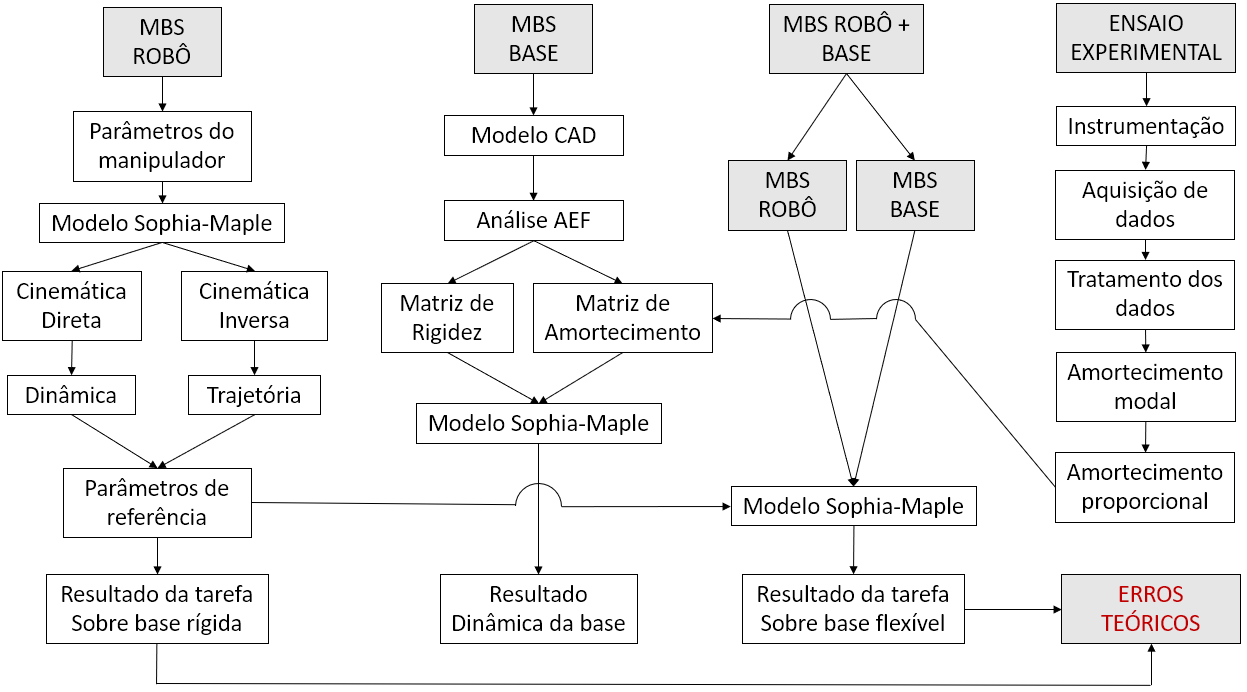
\includegraphics[width=0.99\textwidth]{figs/visgeral}
 	\caption{Diagrama da visão geral do método}
 	\label{fig::visgeral}
\end{figure}



% -.~.-.~.-.~.-.~.-.~.-.~.-.~.-.~.-.~.-.~.-.~.-
\section{Modelo do robô} \label{sec::robo}

% Nesta seção, são detalhados os procedimentos para representar o manipulador
% robótico como um conjunto MBS e utilizá-lo para simular as trajetórias
% referentes a uma determinada tarefa. O manipulador será descrito pelo conjunto
% de Sistemas de Coordenadas (SC's) referente a cada uma de suas juntas, pelas
% distâncias entre os SC's e posição dos centros de massa de cada elo, e pelos
% parâmetros de massa e momento de inércia de cada elo. Os elos do robô e a
% ferramenta acoplada no efetuador representam cada corpo do sistema MBS. A
% modelagem do manipulador é simplificada utilizando as rotinas de CAS
% desenvolvida especialmente para MBS, o Sophia, assim como a notação algébrica de
% Lesser, apresentada na seção~\ref{sec::sophia-kane}.

\subsection{Descrição do braço robótico} \label{sec::descricao_mh12}

O manipulador escolhido para estudo é o mesmo que será utilizado no projeto
EMMA. Trata-se de um robô comercial da série MOTOMAN, modelo MH12, fabricado
pela Yaskawa Motoman e é apresentado na Figura~\ref{fig::mh12_foto}.

\begin{figure}[h]
    \centering
    \begin{subfigure}[b]{0.3\textwidth}
        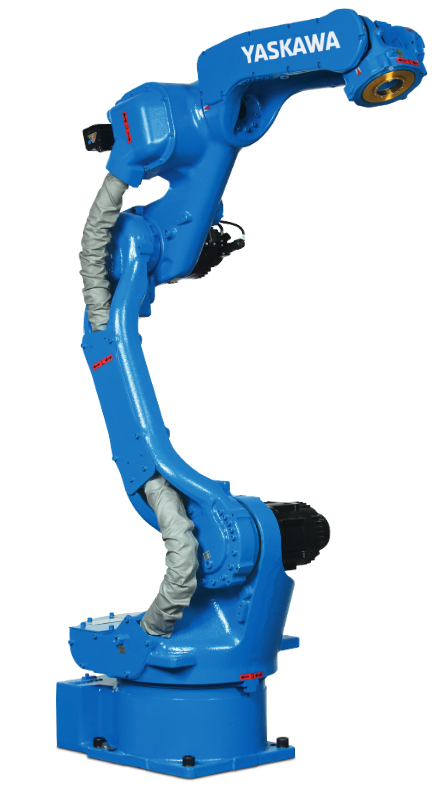
\includegraphics[width=\textwidth]{figs/mh12_foto}
        \caption{MOTOMAN MH12}
        \label{fig::mh12_foto}
    \end{subfigure}
    \quad %add desired spacing between images, e. g. ~, \quad, \qquad, \hfill
    % etc.
      %(or a blank line to force the subfigure onto a new line)
    \begin{subfigure}[b]{0.5\textwidth}
        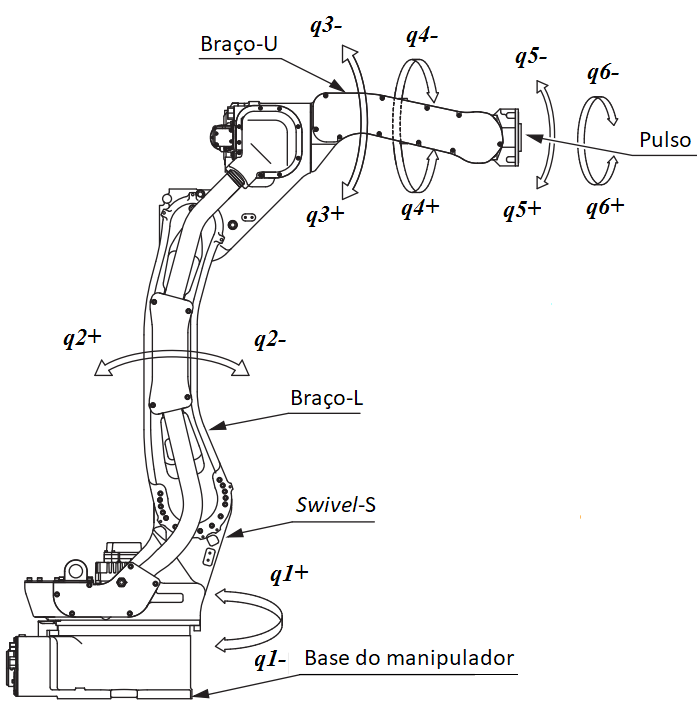
\includegraphics[width=\textwidth]{figs/mh12_diagram}
        \caption{Diagrama dos elos e juntas}
        \label{fig::mh12_diagram}
    \end{subfigure}
    \caption[Manipulador robótico para modelo]{Manipulador robótico para modelo.
    \\Fonte: adaptada de~\cite{manualmh12}}
    \label{fig::resumo_mh12}
\end{figure}

\begin{table}[h]
\centering
\caption{Sistemas de coordenadas, elos e coordenadas generalizadas}
\label{tab::resumo_mh12}
\begin{tabular}{@{}clc@{}}
\toprule
SC & Elo              & \multicolumn{1}{l}{Coord. gen. associada} \\ \midrule
Z  & Pedestal do robô & -                                         \\
S  & \textit{Swivel}  & q1                                        \\
L  & Braço inferior   & q2                                        \\
U  & Braço superior   & q3                                        \\
R  & Braço de rolagem & q4                                        \\
B  & Pulso            & q5                                        \\
T  & Efetuador        & q6                                        \\ \bottomrule
\end{tabular}
\end{table}

Este robô é do tipo braço antropomórfico de 6 juntas rotacionais, e portanto 6
graus de liberdade (6 gdl), contendo o último elo um porta-ferramentas que
suporta uma carga útil de até 12 kg. A Figura~\ref{fig::mh12_diagram} define
os nomes dos elos e coordenadas generalizadas associados a cada um dos sistemas
de coordenadas e são resumidos na Tabela~\ref{tab::resumo_mh12}.

A última junta, no efetuador, tem a finalidade de orientar a ferramenta em torno
do seu eixo axial. Como o processo de revestimento por HVOF independe desta
orientação, esta junta \emph{não será incluída} no modelo MBS do robô, mantendo
este acoplamento rígido, o que transforma os dois últimos elos e a ferramenta
acoplada em um único um corpo. Como resultado, tem-se um sistema de 5 gdl. Outra
observação importante é que o pedestal do robô não realiza movimento em relação
ao referencial SC-Z, que no modelo de base rígida é o próprio referencial
inercial.

O espaço de trabalho é apresentado na Figura~\ref{fig::workspace} em que a área
sombreada é formada por todos os pontos alcançáveis pelo manipulador, dentro dos
limites de cada junta. O alcance horizontal deste manipulador chega a 1,440~m, e
vertical a 2,511~m.

\begin{figure}[h]
	\centering 
 	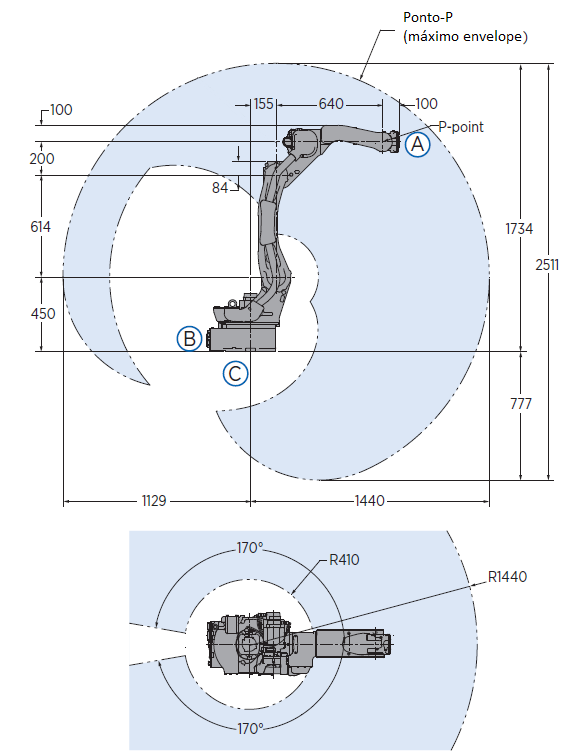
\includegraphics[width=0.65\textwidth]{figs/workspace}
 	\caption[Vistas lateral e superior do espaço de trabalho]{Vistas lateral e
 	superior do espaço de trabalho \\Fonte: adaptada de~\cite{manualmh12}}
 	\label{fig::workspace}
\end{figure}


\subsection{Cinemática Direta}\label{sec::dkin}

Como foi discutido na seção~\ref{sec::cinematica}, o procedimento mais utilizado
para a modelagem cinemática de manipuladores robóticos é o método dos parâmetros
de Denavit-Hartenberg. Apesar de sua popularidade e vasta utilização na
modelagem cinemética de manipuladores variados, as rotinas de modelagem da
cadeia cinemática do Sophia-Maple será utilizado, uma vez que já fornece
praticidade e flexibilidade para derivar as equações cinemáticas de sistemas
multicorpos com mais liberdade que o método DH. Uma vantagem é não ficar
preso às restrições sobre a escolha dos referenciais por exemplo, permitindo
investigar outras configurações que inclusive possam melhorar a eficiência das
manipulações algébricas dadas as particularidades de cada sistema.

Demonstra-se portanto os procedimentos para modelagem de um manipulador robótico
pelas rotinas do Sophia-Maple. A cada etapa são apresentadas as linhas de código
correspondentes, a fim de ilustrar a sistematicidade e praticidade do método.

\subsubsection{Sistemas de Coordenadas}

A primeira etapa para é definir o sistema de coordenadas local de cada elo do
manipulador. A Figura~\ref{fig::scs} é um modelo CAD do braço robótico e
apresenta a posição de cada SC, na sua configuração inicial.

\begin{figure}[h]
    \centering
    \begin{subfigure}[b]{0.20\textwidth}
        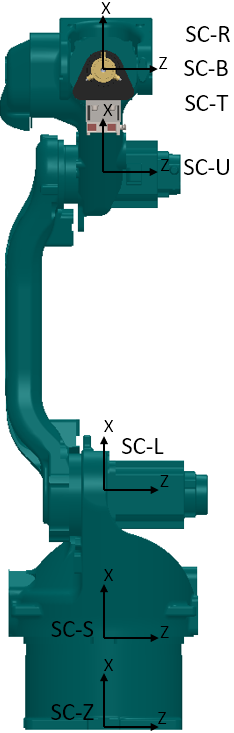
\includegraphics[width=\textwidth]{figs/sc_front}
        \caption{Vista frontal}
        \label{fig::sc_front}
    \end{subfigure}
    \quad %add desired spacing between images, e. g. ~, \quad, \qquad, \hfill
    % etc.
      %(or a blank line to force the subfigure onto a new line)
    \begin{subfigure}[b]{0.7\textwidth}
        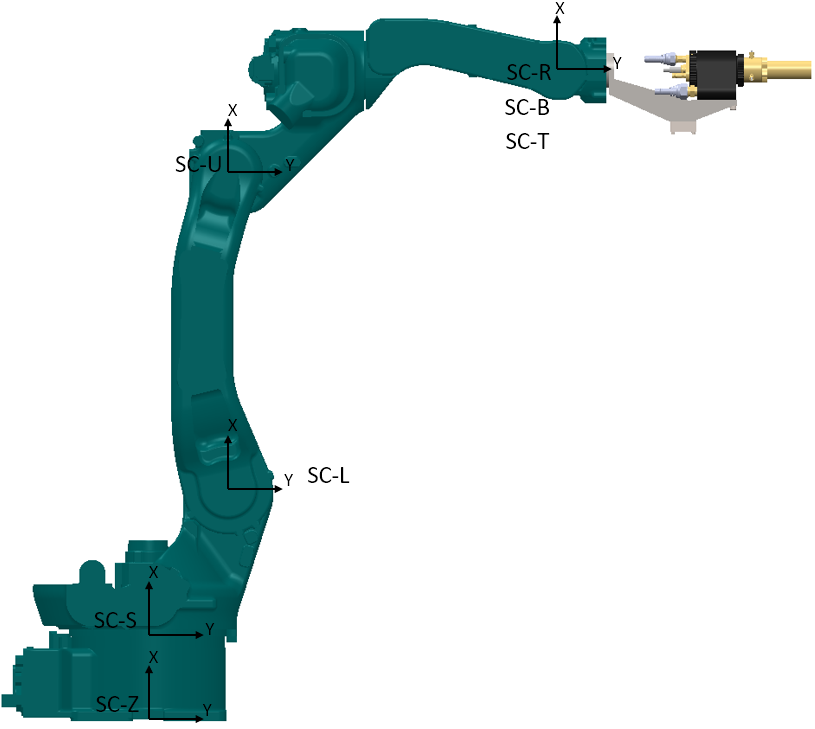
\includegraphics[width=\textwidth]{figs/sc_lat}
        \caption{Vista lateral}
        \label{fig::sc_lat}
    \end{subfigure}
    \caption{Sistemas de coordenadas do robô}\label{fig::scs}
\end{figure}

Na Figura~\ref{fig::sc_front} nota-se que foi escolhida uma configuração em que
todos os SC's estão no mesmo plano $xz$. Outra observação é que os SC's R,
B e T estão fixados no mesmo ponto. que representa a origem do ``pulso'' do
braço robótico. Estas considerações reduzem a quantidade de termos das equações
cinemáticas. Também terão grande impacto no cálculo da cinemática inversa, como
será visto na seção~\ref{sec::ikin_mh12}.

Logo, pode-se escrever as relações entre estes referenciais em termos das
coordenadas generalizadas do sistema, e obter as transformações homogêneas entre
cada SC. No Sophia-Maple isto é feito com o uso da função \texttt{chainSimpRot},
da seguinte forma:

\bigskip \noindent {\tt > chainSimpRot( [Z,S,1,q1], [S,L,3,q2], [L,U,3,q3],
[U,R,2,q4], [R,B,3,q5], [B,T,2,q6] )} \bigskip 

Esta função cria as matrizes de rotação entre os referenciais do sistema,
informando a cada transformação, o eixo de rotação
(onde $1 \equiv x$, $2 \equiv y$ e $3 \equiv z$) e a coordenada generalizada
associada (q1,~\ldots~,q6).

Como exemplo, considere o termo {\tt [L,U,3,q3]}. Representa uma rotação de um
ângulo q3, do SC-U em relação ao SC-L, em torno do eixo Z.
Logo, a matriz rotação entre o referencial inercial Z e o braço
superior U seria:
%
$$ R_{Z}^{U} = R_{Z}^{S} R_{S}^{L} R_{L}^{U} $$
%
A função \texttt{Rmx} do Sophia-Maple retorna a matriz de rotação entre quaisquer
sistemas de coordenadas. No Sophia-Maple, escreve-se:

\bigskip \noindent {\tt > Rmx(Z,U)} \bigskip 

E obtém-se o resultado:
%
$$ R_{Z}^{U} = \left( \begin {array}{ccc} {\it c2}\,{\it c3}-{\it s2}\,{\it
s3}&-{ \it c2}\,{\it s3}-{\it s2}\,{\it c3}&0\\ \noalign{\medskip}{\it c1}\,{
\it c2}\,{\it s3}+{\it c1}\,{\it s2}\,{\it c3}&{\it c1}\,{\it c2}\,{
\it c3}-{\it c1}\,{\it s2}\,{\it s3}&-{\it s1}\\ \noalign{\medskip}{
\it s1}\,{\it c2}\,{\it s3}+{\it s1}\,{\it s2}\,{\it c3}&{\it s1}\,{
\it c2}\,{\it c3}-{\it s1}\,{\it s2}\,{\it s3}&{\it c1}\end {array}
 \right) $$
 %
 A matriz acima foi escrita em notação trigonométrica simplificada, em que c1,
 s1, ,c2, s2, \ldots, e assim por diante, representam as funções senos e
 cossenos dos ângulos das coordenadas generalizadas q1, \ldots, q5. Para melhor
 visualização das matrizes e equações, esta notação será utilizada em todo o
 texto.
 
\subsubsection{Vetores posição e centros de massa}

A segunda etapa é definir os vetores posição dos centros de massa de cada corpo.
Para isso, define-se auxiliarmente os vetores posição entre cada sistema de
coordenada, desde o referencial inercial SC-Z até o efetuador em SC-T, de
acordo com a equação~\ref{eq::posjnutas}.

Logo, de maneira geral, pode-se escrever a posição de qualquer ponto pela
seguinte relação:
%
\begin{align}
	^{Z}\mathbf{p}^{k} &= ~^{Z}\mathbf{p}^{k-1} + ~^{k-1}\mathbf{p}^{k}
	\label{eq::posjnutas} \\
	^{Z}\mathbf{pcm}^{k} &= ~^{Z}\mathbf{pcm}^{k-1} + ~^{k}\mathbf{pcm}
	\label{eq::pcm}
\end{align}
%
Onde $^{Z}\mathbf{p}^{k}$ é o vetor posição do referencial $k$ em relação ao
referencial inercial $Z$ e analogamente $^{Z}\mathbf{pcm}^{k}$ é o vetor
posição do centro de massa do corpo $k$, tal que $k$ varia em \{S,L,U,B,T\},
os sistemas de coordenadas do robô.
No Sophia-Maple é utilizada a notação de Lesser, por meio dos \texttt{Evectors},
para representar esses vetores, como descrito na seção~\ref{sec::lesser}. Logo,
as equações~\ref{eq::posjnutas} são definidas pela seguinte
estrutura:

\bigskip \noindent {\tt > pZ:= Evector(0,0,0,Z);} \\
\noindent {\tt > for k from corpo[1] to corpo[6] do \\
\indent p||k:= p||{k-1} \&++ Evector(p||{k-1}||{k}||x, p||{k-1}||{k}||y,
\indent p||{k-1}||{k}||z, k-1) \\
end do:} \bigskip 

E para as equações~\ref{eq::pcm}, os centros de massa:

\bigskip \noindent {\tt > for k from corpo[1] to corpo[6] do \\
\indent pcm||k:= p||{k} \&++ Evector(pcm||{k}||x, pcm||{k}||y, pcm||{k}||z, k)
\\ end do:} \bigskip 

A Figura~\ref{fig::amb3D} apresenta o ambiente de simulação 3D, criado para
facilitar a visualização do posicionamento e movimento das juntas e elos do
robô. Definidos os pontos de origem de cada referencial, representa-se os elos
do manipulador por uma linha colorida entre os SC's. A ferramenta acoplada é
representada por uma linha que se estende desde a origem do pulso até sua
extremidade. 

Neste ambiente 3D é possível fornecer qualquer configuração de juntas e obter-se
um resultado visual de posicionamento e orientação dos elos. A
Figura~\ref{fig::amb3D_posA} ilustra o resultado para a configuração inicial do
do robô, $q1 = \ldots = q6 = 0$; e a Figura~\ref{fig::amb3D_posB} para a
configuração $q1 = \ldots = q6 = {-}^{\pi}/_2$.

\begin{figure}[h]
    \centering
    \begin{subfigure}[b]{0.4\textwidth}
        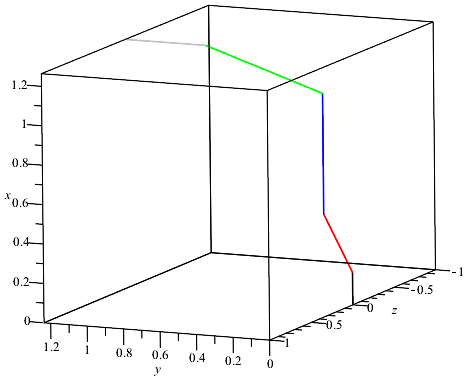
\includegraphics[width=\textwidth]{figs/amb3D_posA}
        \caption{Configuração inicial}
        \label{fig::amb3D_posA}
    \end{subfigure}
    \quad %add desired spacing between images, e. g. ~, \quad, \qquad, \hfill
    % etc.
      %(or a blank line to force the subfigure onto a new line)
    \begin{subfigure}[b]{0.45\textwidth}
        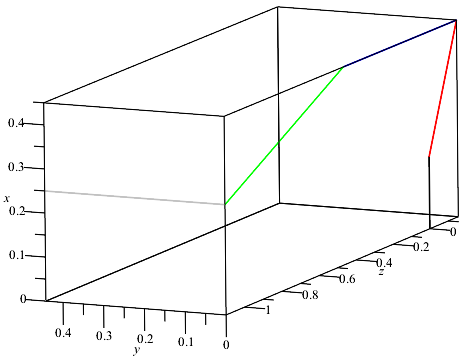
\includegraphics[width=\textwidth]{figs/amb3D_posB}
        \caption{Configuração $q1 = \ldots = q6 = {-}^{\pi}/_2$}
        \label{fig::amb3D_posB}
    \end{subfigure}
    \caption{Ambiente 3D de visualização do robô}\label{fig::amb3D}
\end{figure}

\subsubsection{Velocidades}

As velocidades dos centros de massa de cada corpo são calculadas como a derivada
do vetor posição com respeito ao referencial inercial. Logo, a derivada da
equação~\ref{eq::pcm} em Z:
%
\begin{equation} \label{eq::veloc}
	\mathbf{v}^{k} = \frac{^{Z}\mathrm{d} }{\mathrm{d} t}
	\mathbf{pcm}^{k} 
\end{equation}
%

A função \texttt{cdft}, do Sophia realiza a diferenciação vetorial dos
\texttt{Evectors} com relação ao referencial inercial. Logo, pode-se escrever o
seguinte comando para definir as velocidades de cada corpo de acordo com a
equação~\ref{eq::veloc}:

\bigskip \noindent {\tt > for k from corpo[1] to corpo[6] do \\
\indent v||k:= cdft(pcm||{k}, Z) \\
end do:} \bigskip 

As velocidades angulares são a taxa de variação angular das matrizes de rotação
entre os referenciais. São definidas as velocidades angulares de cada corpo em
relação ao referencial inercial. Pode-se escrever a velocidade angular de uma
matriz rotação $R(t)$ como:
%
\begin{equation} \label{eq::velang}
	\frac{\mathrm{d} R}{\mathrm{d} t} = S \cdot R(t)
\end{equation}
%
Onde $S$ é o tensor velocidade angular associado a $\omega$.
%
\begin{align}
% eq1
& S = \begin{pmatrix}
0				& -\omega_{z}(t)	& \omega_{y}(t) \\ 
\omega_{z}(t)	& 0					& -\omega_{x}(t) \\ 
-\omega_{y}(t)	& \omega_{x}(t)		& 0
\end{pmatrix} \\
% eq2
& \boldsymbol{\omega} = [\omega_{x}, \omega_{y}, \omega_{z}]
\end{align}
%
No Sophia-Maple o tensor $S$ é calculado através da função
\&\texttt{VtoD}. Por exemplo, o tensor entre os referenciais SC-L e SC-S seria:
%
$$
S_{L}^{Z} = \left( \begin {array}{ccc} 0&-{\it q2t}&-\sin \left( {\it q2}
 \right) {\it q1t}\\ \noalign{\medskip}{\it q2t}&0&-\cos \left( {\it 
q2} \right) {\it q1t}\\ \noalign{\medskip}\sin \left( {\it q2}
 \right) {\it q1t}&\cos \left( {\it q2} \right) {\it q1t}&0
\end {array} \right)
$$
%
Pode-se ainda fazer o uso da função \texttt{aV} que
calcula diretamente o vetor velocidade angular $^{A}\omega^{B}$ entre dois
referenciais. O que retornaria, para o exemplo proposto, o seguinte vetor:
%
$$
^{Z}\boldsymbol{\omega}^{L} = [-{\it q1t},\sin \left( {\it q1} \right) {\it q2t},-\cos
\left( {\it q1} \right) {\it q2t}]
$$
%
No caso do manipulador, são calculadas as velocidades de cada corpo em relação
ao referencial Z. São definidas da seguinte forma:

\bigskip \noindent {\tt > for k from corpo[1] to corpo[6] do \\
\indent w||k:= aV(Z, corpo[k]) \\
end do:} \bigskip 

Finalmente, escreve-se o vetor Velocidades Generalizadas, que nada mais é
que um \texttt{Kvector} formado pela lista de \texttt{Evectors} referente às
velocidades lineares e angulares calculadas. Logo, o vetor velocidades
generalizadas tem a seguinte forma:
%
\begin{equation}
	\mathbf{v}_{g} = [ \mathbf{v}^{S},\ldots, \mathbf{v}^{T}, \boldsymbol{\omega}^{S},\ldots,
	\boldsymbol{\omega}^{T}]
\end{equation}
%
Onde cada termo do \texttt{Kvector} é um \texttt{Evector} da velocidade
generalizada.

\subsubsection{Hiperplano tangente}

Uma vez que as velocidades generalizadas foram definidas pode-se obter o
conjunto de vetores tangentes, pelo cálculo das velocidades parciais, que formam
o chamado hiperplano tangente, $\tau$, conforme demonstrado na
seção~\ref{sec::sophia_kane}.

A função \texttt{KMtangents} do Sophia-Maple obtém os termos que formam os
vetores tangentes em \texttt{Kvectors} para cada coordenada generalizada. O
conjunto que forma o hiperplano tangente introduz uma estrutura do Sophia, dos
super \texttt{Kvectors}, ou \texttt{SKVector}. Esta estrutura facilitará a
projeção das equações dinâmicas no hiperplano tangente. Logo, para o manipulador
escreve-se simplesmente:

\bigskip \noindent {\tt > tau:= KMtangents(vK,u,6):} \bigskip


\subsection{Dinâmica}

Definida a cinemática direta do manipulador, deseja-se obter as forças de
inércia e externas generalizadas que fornecerão as equações de movimento do
sistema.

\subsubsection{Parâmetros de inércia do manipulador robótico}

Os parâmetros de inércia são a massa e o momento de inércia de cada corpo do
sistema. É importante notar que não é possível obter um modelo dinâmico preciso
apenas com as informações contidas nos manuais e fichas técnicas do robô.
Infelizmente os parâmetros de inércia individuais de cada corpo não são
fornecidos pelos fabricantes e, portanto, serão estimados pelo método a seguir.

Do manual do MOTOMAN MH12~\cite{manualmh12}, informa-se a massa total do robô,
de 130~kg. Também é disponibilizado, diretamente pelo fabricante, um modelo CAD
com ótimo detalhamento de cada corpo individualmente.

Pelo modelo CAD no programa SolidWorks é possível obter o volume $V_k$ de cada
elo $k$ em separado. Com isso, calcula-se a massa específica média do robô, de
acordo com a equação~\ref{eq::rho}.
%
\begin{align}
	\rho_{m} = M_{total}\sum_{k = Z}^{T} V_{k} \label{eq::rho} \qquad & ,
	k = Z,S,L,U,R,B,T
\end{align}
%
Em seguida, estima-se a massa de cada corpo, calculada pelo produto da massa
específica média $\rho_{m}$ e o seu volume, de acordo com a
equação~\ref{eq::massai}.
%
\begin{align}
	m_{k} = \rho_{m} \cdot V_{k} \label{eq::massai} \qquad &, k =
	Z,S,L,U,R,B,T
\end{align}
%
A massa da ferramenta acoplada ao efetuador foi obtida de forma precisa,
pelo projeto do suporte, e informação do fabricante do dispositivo
HVOF.
A Tabela~\ref{tab::massa_mh12} apresenta os resultados da massa estimada em cada
corpo:
%
\begin{table}[h]
\centering
\caption{Resultado do cálculo da massa de cada corpo}
\label{tab::massa_mh12}
\begin{tabular}{@{}clc@{}}
\toprule
\textbf{Corpo}                      & \textbf{Volume} [$m^3$] & \multicolumn{1}{l}{\textbf{Massa} [kg]} \\ \midrule 
Z 									& 0,01595         & 40,5							   \\
S                                   & 0,01443         & 36,7                               \\
L                                   & 0,00579         & 14,7                               \\
U                                   & 0,00997         & 25,3                               \\
R                                   & 0,00399         & 10,1                               \\
B                                   & 0,00100         & 2,5                                \\
T                                   & 0,00005         & 0,13                               \\
Ferramenta                          & -		          & 5,97							   \\ \midrule
\textbf{Volume total}~$=$           & 0,05119        & \multicolumn{1}{c}{$m^3$}	       \\
\multicolumn{1}{r}{\textbf{$\rho_m =$}} & 2540          &
\multicolumn{1}{c}{$kg/{m^3}$}     \\ \bottomrule
\end{tabular}
\end{table}
%

Para este modelo dinâmico, não será utilizada a última junta do robô, como foi
explicado na seção~\ref{sec::descricao_mh12}. Assim, para os corpos ``B, T e
Ferramenta'', as propriedades de massa e momento de inércia podem ser somadas e
condensadas em uma única descrição.

A partir deste ponto do texto, estes 3 últimos corpos serão tratadaos como um
único corpo e será utilizada a denominação do corpo B para representar esse conjunto.

Do modelo CAD do MH12 também é possível extrair as posições do centro de massa e
momentos de inércia de cada elo. Como foi considerado que a massa é distribuida
homogeneamente no volume de cada corpo, resulta-se numa posição estimada do
centro de massa. A Tabela~\ref{tab::resumo_cm} resume os valores encontrados
para a posição do centro de massa com respeito ao referencial local de cada elo
e a Figura~\ref{fig::pcm_mh12} ilustra a posição aproximada.

\begin{figure}[h]
	\centering 
 	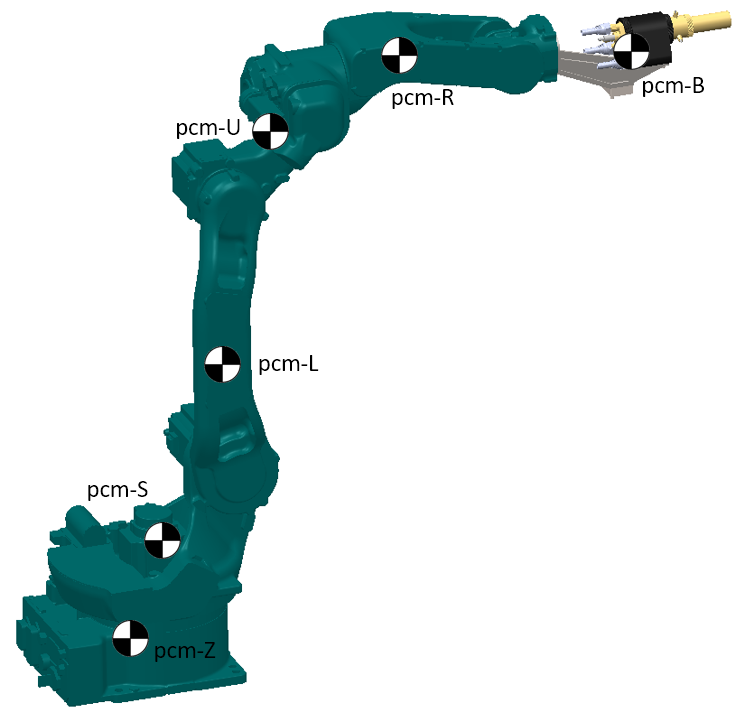
\includegraphics[width=0.5\textwidth]{figs/pcm_mh12}
 	\caption{Posição aproximada dos centros de massa}
 	\label{fig::pcm_mh12}
\end{figure}

%
\begin{table}[h] \centering
\caption{Posição do centro de massa de cada corpo}
\label{tab::resumo_cm}
\begin{tabular}{@{}cccc@{}}
\toprule
\textbf{Corpo} & \textbf{x [m]} & \textbf{y [m]} & \textbf{z [m]} \\ \midrule
Z              & 0,079      & -0,050     & 0,000      \\
S              & 0,124      & 0,027      & 0,008      \\
L              & 0,281      & -0,025     & -0,115     \\
U              & 0,123      & 0,115      & -0,025     \\
R              & 0,039      & -0,224     & 0,004      \\
B              & -0,011     & 0,146      & 0,000      \\ \bottomrule
\end{tabular}
\end{table}
%

O SolidWorks calcula os momentos de inércia obtidos no centro de massa e
alinhados ao sistema de coordenadas local de cada elo.
O resultado do cálculo dos momentos de inércia são apresentados a seguir.
%
\begin{align*}
InZ &=& \left( \begin {array}{ccc}  0,811& 0,293& 0,091\\ \noalign{\medskip}
 0,293& 0,695& 0,064\\ \noalign{\medskip} 0,091& 0,064& 0,923
\end {array} \right) & \quad InS &=& \left( \begin {array}{ccc}  0,811& 0,293& 0,091\\ \noalign{\medskip}
 0,293& 0,695& 0,064\\ \noalign{\medskip} 0,091& 0,064& 0,923
\end {array} \right) \\
InL &=&  \left( \begin {array}{ccc}  0,051&-
0,008&- 0,032 \\ \noalign{\medskip}- 0,008& 0,791& 0,011\\ \noalign{\medskip}- 0,032
& 0,011& 0,798\end {array} \right) & \quad InU &=& \left( \begin {array}{ccc} 
0,314& 0,149&- 0,077\\ \noalign{\medskip} 0,149& 0,367&- 0,057\\ \noalign{\medskip}- 0,077&- 0,057& 0,418
\end {array} \right) \\
InR &=&  \left( \begin {array}{ccc}  0,173&-
0,014& 0,001\\ \noalign{\medskip} - 0,014& 0,052& 0,004\\ \noalign{\medskip} 0,001& 0,004& 0,148
\end {array} \right) & \quad InB &=&  \left( \begin {array}{ccc}  0,235&- 0,018& 0,0\\ \noalign{\medskip}-
 0,018& 0,039& 0,0\\ \noalign{\medskip} 0,0& 0,0& 0,243\end {array}
 \right)
\end{align*}
%
No Sophia-Maple estes tensores são construidos com a função
\texttt{EinertiaDyad}, que aproveita o fato dos tensores de inércia serem
simétricos e recebe 6 argumentos para os termos da matriz e um para especificar
o sistema de coordenadas de referência em que foi obtido o tensor. Define-se
portanto cada tensor da seguinte forma:

\bigskip \noindent {\tt > for i from corpo[1] to corpo[6] do \\
\indent In||(corpo[i]):= EinertiaDyad( \\
\indent In||(corpo[i])||11, In||(corpo[i])||22, \\
\indent In||(corpo[i])||33, In||(corpo[i])||12, \\
\indent In||(corpo[i])||13, In||(corpo[i])||23, sc[i]) \\
end do:}

\subsubsection{Quantidade de Movimento e Quantidade de Movimento Angular}

Para o cálculo das forças de inércia, calcula-se a Quantidade de Movimento $G$ e
a Quantidade de Movimento Angular $H$, para cada corpo, de acordo com as
equações~\ref{eq::qntmov} e \ref{eq::qntmovang}.
%
\begin{align}
%eq1
	\mathbf{G}_{k} &= m_{k} \cdot \mathbf{v}_{k} \label{eq::qntmov} \\
%eq2	
	\mathbf{H}_{k} &= In_{k} \cdot \boldsymbol\omega^{k} \label{eq::qntmovang}
\end{align}
%

\subsubsection{Forças de Inércia}

As forças de inércia são a derivada temporal das quantidades de movimento, com
respeito ao referencial inercial Z, conforme descrito pelas
equações~\ref{eq::finG} e \ref{eq::finH}.
%
\begin{align}
%eq1
	\dot{\mathbf{G}}_{k} &= \frac{^{Z}\mathrm{d}}{\mathrm{d} t} (m_{k} \cdot
	\mathbf{v}_{k}) \label{eq::finG} \\
%eq2	
	\dot{\mathbf{H}}_{k} &= \frac{^{Z}\mathrm{d}}{\mathrm{d} t} (In_{k} \cdot
	\mathbf{\boldsymbol\omega^{k}}_{k}) \label{eq::finH}	
\end{align}
%
No Sophia-Maple, obtém-se primeiro os vetores quantidade de movimento e, em
seguida. Constrói-se o \texttt{Kvector} das quantidades de movimento
generalizadas através da função \texttt{KM}, e armazena este na variável
\texttt{KMG}. Por fim, é usada a função \texttt{Kfdt} para diferenciação
temporal das quantidades de movimento generalizadas e obtenção do vetor das
Forças de Inércia, \texttt{FIN}.

% Vale notar que o Sophia-Maple adiciona um sufixo t aos termos que foram
% derivados com respeito ao tempo.
% Logo, as coordenadas generalizadas, q1,\ldots,qn, quando derivadas no tempo
% resultam em q1t,\ldots,qnt. Este formato auxilirá a substituição destes termos
% para solução das \textit{kinematic differential equations} (kde), conforme visto
% na seção~\ref{sec::sophia-kane}.

% O algoritmo para definir as Forças de Inércia do sistema no Sophia-Maple é o
% seguinte:

\bigskip \noindent {\tt > for i from 1 to 6 do \\
\indent G||corpo[i]:= m||corpo[i] \&** v||corpo[i] \\
end do: \# Define as Quantidades de Movimento}

\medskip \noindent {\tt > for i from 1 to 6 do \\
\indent H||corpo[i]:= In||corpo[i] \&** w||corpo[i] \\
end do: \# Define as Quantidades de Movimento Angular}

\medskip \noindent {\tt > KMG:= subs(kde, KM[G||corpo, H||corpo]): \\
\# Define o Kvector das Quantidades de Movimento generalizadas}

\medskip \noindent {\tt > FIN:= subs(kde, Z Kfdt KMG): \\
\# Define o Kvector das Forças de Inércia}


\subsubsection{Forças Externas}

Uma das vantagens do método de Kane é não ser necessário avaliar as forças
internas, ou de restrição entre os corpos dos sistema. O motivo é que, ao se
projetarem as equações de equilíbrio dinâmico no hiperplano tangente, $\tau$,
essas forças desaparecem.

Logo, apenas as forças externas precisam ser modeladas para obter as equações de
movimento. No modelo do braço robótico, estas forças são o peso, os torques das
juntas e os torques de controle PID, em cada elo.

A força peso atua aplicada ao centro de massa de cada corpo \textit{k} e é calculada
pela equação~\ref{eq::peso}:
%
\begin{equation}
	\mathbf{Peso}_{k} = m_{k} \cdot \mathbf{g} \label{eq::peso}
\end{equation}
%
Onde $\mathbf{g}$ refere-se ao vetor da aceleração da gravidade, que atua sempre
no sentido de $-x$ no referencial inercial SC-Z. É definido como:
%
\begin{equation}
	\mathbf{g} = [-9,81,~0,~0]^{Z}
\end{equation}
%
Os momentos externos são formados pelos torques dos atuadores em cada junta e
também os torques de controle PID. Neste momento é válido acrescentar uma
explicação rápida sobre a modelagem do controlador PID.

\subsubsection{Parâmetros de controle PID}

Para que o robô realize a tarefa, é necessário seguir a trajetória previamente
planejada. Uma trajetória pode ser simplesmente um conjunto de posições e
velocidades de referência de cada junta, que variam no tempo, como foi abordado
na seção~\ref{sec::plan_traj}. A variação das posições se dá pelo acionamento
dos torques em cada junta, que deve ser controlado para seguir a trajetória
planejada.

Os fabricantes de robôs comerciais infelizmente não fornecem detalhes sobre o
método nem os parâmetros de controle utilizados.
Com o propósito de simular o controle do manipulador decidiu-se pela
simplicidade do método de controle PID.

Logo, define-se as equações dos torques de controle para cada junta, em função
da diferença entre os parâmetros instantâneos e os de referência em cada junta.
O subíndice $k$ representa a lista de juntas, localizada na origem de cada
sistema de coordenadas de mesmo nome, variando em \{S,L,U,R,B\} e o
subíndice $i$ o número da coordenada generalizada associada.
%
\begin{equation}
	PID_{k} = Kp(q_i-q_i{ref}) + Ti\int_{t1}^{t2} (q_i-q_i{ref})dt +
	Td(u_i-u_i{ref}) \label{eq::pid}
\end{equation}
%

Os parâmetros de controle PID são formados pelas variáveis proporcional,
integral e derivativa, $Kp$, $Td$ e $Ti$ respectivamente. Esses parâmetros
foram sintonizados para cada junta individualmente, fazendo-se simulações de
resposta para uma função degrau de referência. 

Como resultado da análise, encontrou-se os melhores resultados para o conjunto
de parâmetros apresentados na Tabela~\ref{tab::pid}:
%
\begin{table}[h]
\centering
\caption{Parâmetros de controle PID em cada junta}
\label{tab::pid}
\begin{tabular}{@{}cccc@{}}
\toprule
\textbf{Junta} & \textbf{Kp [kNm]} & \textbf{Ti [kNm]} & \textbf{Td [kNm]} \\ \midrule 
S              & 2		& 8		& 1		\\
L              & 4		& 8		& 1		\\
U              & 4		& 8		& 1		\\
R              & 2		& 1		& 0,15	\\
B              & 2		& 1		& 0,15	\\ \bottomrule
\end{tabular}
\end{table}
%

A Figura~\ref{fig::pid_pi_sobre_2} apresenta o resultado dinâmico para os
valores encontrados considerando uma função degrau de referência de $\pi/2$, em
$t=0~s$, para todas as juntas.

\begin{figure}[h]
	\centering 
 	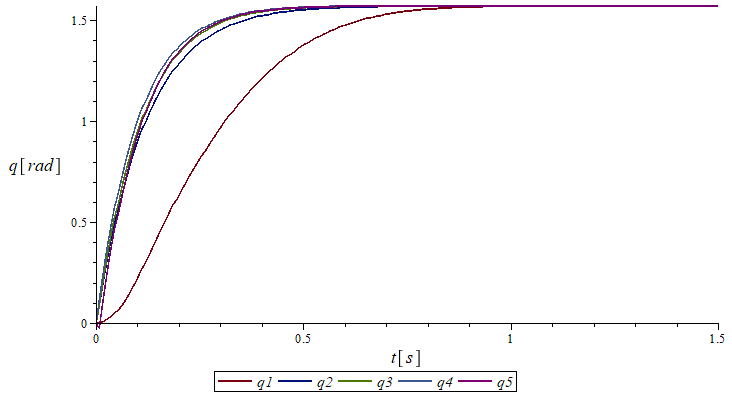
\includegraphics[width=0.90\textwidth]{figs/pid_pi_sobre_2}
 	\caption{Resposta a uma função degrau de $\pi/2$}
 	\label{fig::pid_pi_sobre_2}
\end{figure}

No Sophia-Maple declara-se os torques de controle representados na
equação~\ref{eq::pid} da seguinte forma:

\bigskip \noindent {\tt > for k from 1 to 5 do \\
		 \indent PID\_||{corpo[k]}:= Kp*(q||k - q||k||ref) + Ti*int(q||k - q||k||ref,
		 t) + Td*(u||k - u||k||ref) \\
		 end do:}

\subsubsection{Momentos Externos}

Para obter os momentos externos que atuam em cada corpo, o primeiro passo é
definir os torques que atuam em cada junta. Para eliminar os momentos causados
pelas forças \texttt{Peso}, avaliou-se os torques das juntas com respeito ao
centro de massa de cada corpo. As equações~\ref{eq::tjuntasi} a
\ref{eq::tjuntasf} descrevem os torques externos e de controle que atuam em cada
junta.
\begin{align}
	\mathbf{TjZS} &= (TZS - PID_{S})\cdot[1,~0,~0]^Z \label{eq::tjuntasi} \\
	\mathbf{TjSL} &= (TSL - PID_{L})\cdot[0,~0,~1]^S \\
	\mathbf{TjLU} &= (TLU - PID_{U})\cdot[0,~0,~1]^L \\
	\mathbf{TjUR} &= (TUR - PID_{R})\cdot[0,~1,~0]^L \\
	\mathbf{TjRB} &= (TRB - PID_{B})\cdot[0,~0,~1]^B \label{eq::tjuntasf}
\end{align}
%
As equações~\ref{eq::mexi} a \ref{eq::mexf} calculam o somatório dos momentos
externos em cada corpo. Nota-se que o torque aplicado em qualquer junta causa
um par de torques de ação e reação nos elos adjacentes. As variáveis $Mex_k$ são
vetores que representam o momentos externos resultante em cada
corpo.
%
\begin{align}
	\mathbf{Mex_{Z}} &= - \mathbf{TjZS } \label{eq::mexi}\\
	\mathbf{Mex_{S}} &= \mathbf{TjZS} - \mathbf{TjSL }\\
	\mathbf{Mex_{L}} &= \mathbf{TjLU }- \mathbf{TjSL }\\
	\mathbf{Mex_{U}} &= \mathbf{TjUR }- \mathbf{TjLU }\\
	\mathbf{Mex_{R}} &= \mathbf{TjRB }- \mathbf{TjUR }\\
	\mathbf{Mex_{B}} &= - \mathbf{TjRB} \label{eq::mexf}
\end{align}
%

% Note-se novamente que, pelo método de Kane, não é preciso introduzir as forças
% internas, de restrição ou de contato entre os corpos, porque estas não
% contribuem para as equações de movimento e desaparecem quando o sistema de
% equações de equilíbrio dinâmico são projetads no hiperplano tangente, $\tau$.

No Sophia-Maple os vetores dos momentos externos resultantes são armazenadas em
\texttt{Evectors}. A sequência de equações~\ref{eq::tjuntasi} a \ref{eq::mexf}
torna-se:

\bigskip \noindent {\tt > \# Torques nas juntas} \\
		 \noindent {\tt > TjZS:= Evector(TZS - PID\_S,~0,~0,~S) } \\
		 \noindent {\tt > TjSL:= Evector(0,~0,~TSL - PID\_L,~L) } \\
		 \noindent {\tt > TjLU:= Evector(0,~0,~TLU - PID\_U,~U) } \\
		 \noindent {\tt > TjUR:= Evector(0,~TUR - PID\_R,~0,~R) } \\
		 \noindent {\tt > TjRB:= Evector(0,~0,~TUR - PID\_B,~B) }

\medskip \noindent {\tt > \# Momentos externos em cada elo} \\
		 \noindent {\tt > for k from 1 to 5 do \\
		 \indent Mex||k:= Tj||{k-1}||{k}  - Tj||{k}||{k+1} \\
		 end do:} \\
		 \noindent {\tt > MexB:= - TjRB:} \bigskip

		 
As forças e momentos externos podem ser agrupadas em um único vetor para
auxiliar a projeção destas em $\tau$. Novamente, faz-se uso da função
\texttt{KM}, o que retorna um \texttt{Kvector} contendo todas as forças e
momentos, descritos em cada sistema de referência.

\bigskip \noindent {\tt > FEX:= KM[Fex||corpo,~Mex||corpo]:} \bigskip

A Figura~\ref{fig::sisfex} ilustra, em vista explodida, o equilíbrio das forças e
momentos externos em cada elo do manipulador.

\begin{figure}[h!]
    \centering
    \begin{subfigure}[b]{0.48\textwidth}
        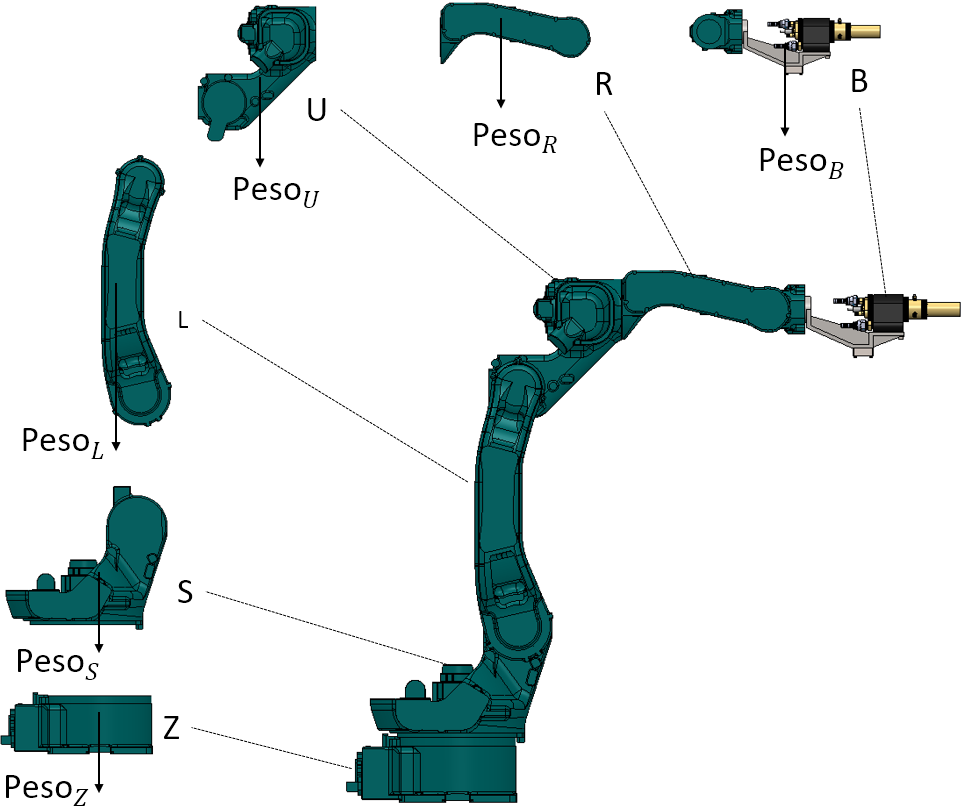
\includegraphics[width=\textwidth]{figs/forcas_ext}
        \caption{Forças externas em cada elo}
        \label{fig::fex}
    \end{subfigure}
    ~ %add desired spacing between images, e. g. ~, \quad, \qquad, \hfill
    % etc.
      %(or a blank line to force the subfigure onto a new line)
    \begin{subfigure}[b]{0.48\textwidth}
        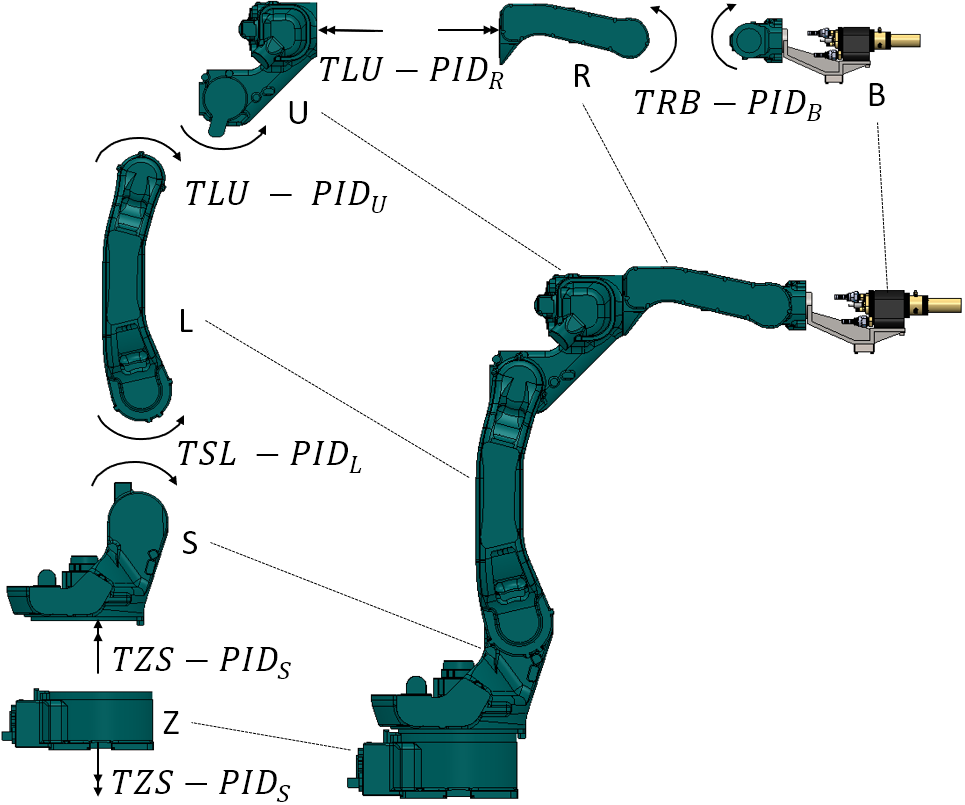
\includegraphics[width=\textwidth]{figs/mom_ext}
        \caption{Momentos externos em cada elo}
        \label{fig::mex}
    \end{subfigure}
    \caption{Sistema de forças externas}\label{fig::sisfex}
\end{figure}

		 
\subsubsection{Forças de Inércia e  Forças Externas Generalizadas}

Estas são as forças externas e de inércia FEX e FIN, quando projetadas no
hiperplano tangente, $\tau$. Para a projeção, faz-se uso da função
\texttt{\&kane}, do Sophia-Maple, o que retorna as equações implícitas
generalizadas de cada corpo:

\bigskip \noindent {\tt > FEXg:= tau \&kane FEX:} \\
		 \noindent {\tt > FINg:= tau \&kane FIN:}
		 
\subsubsection{Equações de Movimento}

Finalmente, as equações de movimento são formadas pelo equilíbrio dinâmico entre
as forças externas e externas generalizadas obtidas da projeção em $\tau$, de
acordo com a equação~\ref{eq::eqdin}:
%
\begin{equation}
	(FINg - FEXg)_{k} = 0 \label{eq::eqdin}
\end{equation}
%
O subíndice \textit{k} representa a lista de corpos \{Z,S,L,U,R,B\}. Como o
corpo Z está fixo no referencial inercial SC-Z, sua equação de movimento
torna-se a solução trivial $0=0$ e portanto, não fará parte do sistema. Obtém-se
então um conjunto de 5 equações de movimento, associadas aos 5 gdl do robô.

No Sophia-Maple atribui-se o conjunto de equações~\ref{eq::eqdin} à
variável \texttt{kane}, formando uma lista das equações de movimento. Portanto:

\bigskip \noindent {\tt > kane:= FINg - FEXg = 0} \bigskip

As equações denominadas \textit{kinematic differential equations}, ou
\texttt{kde}, completam o sistema de equações diferenciais que descrevem o
movimento do robô.
Para os 5 graus de liberdade do manipulador, tem-se 5 kde. As
equações~\ref{eq::kde5i} a \ref{eq::kde5f} descrevem o kde:
%
\begin{align}
	u_{1}(t) &= \frac{\mathrm{d} }{\mathrm{d} t}q_{1}(t) \label{eq::kde5i} \\
	u_{2}(t) &= \frac{\mathrm{d} }{\mathrm{d} t}q_{2}(t) \\
	u_{3}(t) &= \frac{\mathrm{d} }{\mathrm{d} t}q_{3}(t) \\
	u_{4}(t) &= \frac{\mathrm{d} }{\mathrm{d} t}q_{4}(t) \\
	u_{5}(t) &= \frac{\mathrm{d} }{\mathrm{d} t}q_{5}(t) \label{eq::kde5f}	
\end{align}
%

Somando-se esse sistema às equações de movimento e atribuindo à variável
\texttt{eq\_mov}, no Sophia-Maple:

\bigskip \noindent {\tt > eq\_mov:= kane union kde:} \bigskip

Logo, tem-se um sistema de 10 equações diferenciais ordinárias, não-lineares
(equações~\ref{eq::eqdin} a \ref{eq::kde5f}), cujas incógnitas são as
coordenadas generalizadas $q_{1}(t),\ldots, q_{5}(t)$ e as velocidades angulares
$u_{1}(t),\ldots, u_{5}(t)$.

Vale ressaltar que, para o sistema de apenas 5 equações de movimento simbólicas
associadas aos 5 graus de liberdade, as expressões são extensas demais para
serem representadas neste texto, o que ocuparia diversas páginas e obviamente
não traria nenhum valor à discussão deste tópico. Por isso, limita-se a
representação do sistema à equação~\ref{eq::eqdin}.

A função \texttt{cost} do Maple retorna o número de operações algébricas e de
funções de uma determinada equação ou sistema de equações e dá ao usuário um
parâmetro para avaliar o tamanho das expressões e o custo computacional do
modelo.
Para se ter uma ideia, o custo do sistema de equações de movimento, representado
na forma puramente simbólica em \ref{eq::eqdin}, tem  a seguinte estrutura:
%
	$$ 18171\,{\it somas}+59804\,{\it multiplica\c{c}\tilde{o}es}+39998\,{\it 
fun\c{c}\tilde{o}es} $$
%
Porém, lembra-se que o sistema é puramente simbólico, e até então não foram
substituidos os parâmetros numéricos do robô.
Este procedimento simplifica o sistema, porque muitos termos são zerados e
desaparecem.
Além disso, é possível fazer uso da função \texttt{simplify} do Maple, que é um
poderoso conjunto de rotinas para simplificação algébrica de expressões. Fazendo
uso desta função e da substituição dos parâmetros numéricos nas equações de
movimento, obtemos o novo custo algébrico das equações:
%
	$$ 5676\,{\it somas}+6992\,{\it multiplica\c{c}\tilde{o}es}+1835\,{\it fun\c{c}\tilde{o}es} $$
%
Nota-se a grande vantagem de realizar este procedimento, porque ao reduzir-se
drasticamente o número de termos e funções, reduz-se também o custo
computacional e por consequência o tempo para o cálculo da solução.

\subsubsection{Problema de Valor Inicial -- PVI}

Para resolver o sistema diferencial é necessário fornecer as condições de
contorno do problema. Como as equações estão no domínio do tempo, são fornecidas
as condições iniciais das variáveis de estado $q_{1}(0),\ldots, q_{5}(0)$ e
$u_{1}(t),\ldots, u_{5}(0)$.

Será adotado neste modelo que qualquer trajetória será iniciada a partir da
configuração incial do robô, ou seja:
%
\begin{equation}
	q_{1}(0) = \ldots = q_{5}(0) = u_{1}(0) = \ldots = u_{5}(0) = 0
	\label{eq::condini}
\end{equation}
%
O sistema completo será portanto formado pelas 10 equações de movimento
diferenciais e não lineares (\ref{eq::eqdin} a \ref{eq::kde5f}), com as 10
equações de valor incial definidas em~\ref{eq::condini}.

Para definir esse sistema no Sophia-Maple, primeiro cria-se a lista com as
equações de valor inicial e então adiciona-as ao sistema, utilizando a função
\texttt{union}:

\bigskip \noindent {\tt > cond\_ini:= \{seq(q||i(0) = 0, i=1..5), seq(u||i(0) =
0, i=1..5)\}} \\ 
		 \noindent {\tt > sistema:= eq\_mov union condini:} \bigskip

A solução deste sistema depende ainda da definição dos seguintes parâmetros:
%
\begin{itemize}
  \item{Torques nas juntas: TZS, TSL, TLU, TUR, TRB}
  \item{Coordenadas de referência dos ângulos de juntas: 
  		\\ $q_{1}ref, q_{2}ref, q_{3}ref, q_{4}ref, q_{5}ref$}
  \item{Velocidades angulares de referências das juntas: 
  		\\ $u_{1}ref, u_{2}ref, u_{3}ref, u_{4}ref, u_{5}ref$}
\end{itemize}
%
A trajetória efetuada pelo manipulador é então consequência da solução do
sistema, para um conjunto de parâmetros fornecidos. Para realizar uma trajetória
desejada, deve-se fornecer os parâmetros de referência e torques das juntas ao
longo do tempo que resultam naquela trajetória.

Se tal trajetória é descrita pela posição e orientação da ferramenta acoplada ao
último elo do manipulador, os parâmetros das juntas, tais que a ferramenta
segue aquela trajetória, devem ser determinados pelo cálculo da Cinemática
Inversa.


\subsection{Cinemática Inversa}\label{sec::ikin_mh12}

Conforme visto na seção~\ref{sec::ikin}, a solução da cinemática inversa para
este tipo de manipulador pode ser resolvida pelo método geométrico considerando
o modelo desacoplado para posição e orientação.
Logo, resume-se em encontrar os parâmetros das juntas $q_{1}, q_{2}, q_{3}$ que
satisfazem a posição do pulso e $q_{4}, q_{5}, q_{6}$ que satisfazem a
orientação da ferramenta.

A pose final da ferramenta pode ser expressa em termos dos parâmetros
de posição e de orientação, de acordo com a equação~\ref{eq::posf}.
%
\begin{equation}
	\mathbf{x}_{f} = \begin{bmatrix}
		\mathbf{p}_{f} \\ \boldsymbol{\Phi}_{f}
	\end{bmatrix}
	\label{eq::posf}	
\end{equation}
%
Onde:
%
\begin{align}
^Z\mathbf{p}_{f} &= [x_f,y_f,z_f]^Z \\
^Z\boldsymbol{\Phi}_{f} &= [\phi,\theta,\psi]^Z
\end{align}
%



\subsubsection{Cálculo da posição do pulso}

A primeira tarefa é calcular a posição da ferramenta em termos das
coordenadas generalizadas.
Como visto na seção~\ref{sec::ikin}, pode-se expressá-la convenientemente
pela posição da origem do pulso, porque esta só depende das coordenadas $q_1,
q_2$ e $q_3$.

A posição da ponta da ferramenta, $p_{f}$, é então a posição da origem do pulso,
$p_{w}$ em SC-R, somada ao vetor das dimensões da ferramenta, no referencial
SC-B:
%
\begin{equation}
	^Z\mathbf{p}_{f} = \mathbf{p}_{w} + [d_{x}, d_{y}, d_{z}]^B \label{eq::posf}
\end{equation}
%
A Figura~\ref{fig::pwpf} ilustra os vetores posição do pulso e posição da
ferramenta do manipulador MH12.

\begin{figure}[h]
	\centering 
 	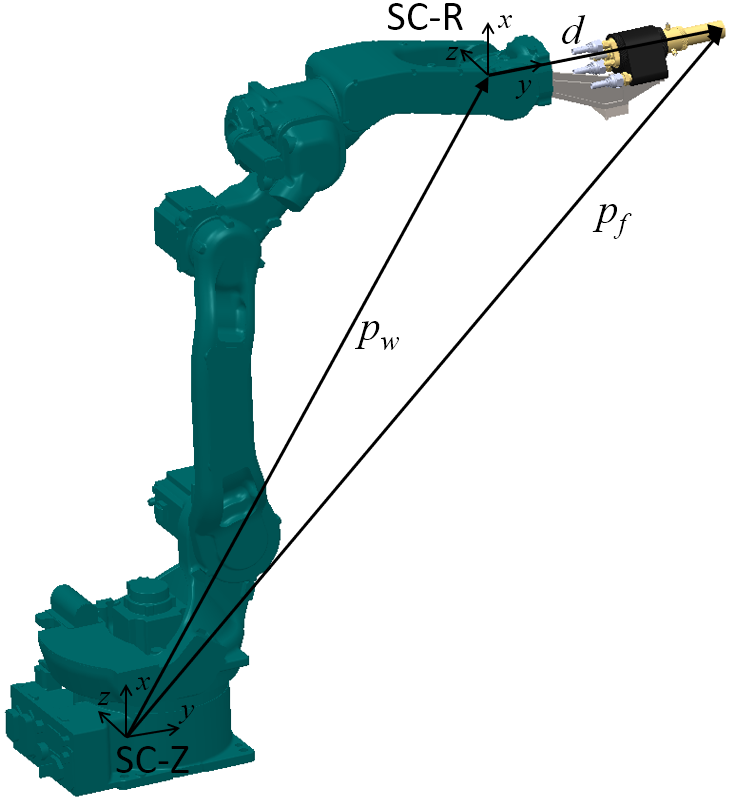
\includegraphics[width=0.45\textwidth]{figs/pwpf}
 	\caption{Posições do pulso e da ferramenta}
 	\label{fig::pwpf}
\end{figure}

Pelo desenvolvimento da cinemática direta, na seção~\ref{sec::dkin}, pode-se
expressar a posição de qualquer ponto da cadeia cinemática em um dado
referencial. Como o pulso tem origem no sistema de coordenadas SC-R, então:
%
\begin{equation} \label{eq::pwpr}
	\mathbf{p}_{w} =~^Z{\mathbf{p}}^R 
\end{equation}
%
Recorrendo às equações~\ref{eq::theta1} a \ref{eq::theta3}, desenvolvidas na
seção~\ref{sec::ikin}, pelo método geométrico, tem-se:
%
\begin{align*}
	q1 &= \atantwo (z_w,y_w) - \atantwo (d, \pm \sqrt{y_w^2 + z_w^2 - d^2}) \\
	q2 &= \atantwo (r,s) - \atantwo (\pm  \sqrt{1-E^2}, E) \\
	q3 &= \atantwo (\pm \sqrt{1-D^2}, D) - \frac{\pi}{2} + \atantwo (h, a3)
\end{align*}
%
Onde:
%
\begin{align*}
	D &= \frac{r^2 + s^2 -a2^2 - a3^2}{2 \cdot a2 \cdot a3} \\
	E &= - \frac{a3^2 - a2^2 - r^2 - s^2}{2 \cdot a2 \cdot \sqrt{r^2 + s^2}}
\end{align*}
%
Uma análise das expressões acima permite relacionar os termos geométricos do
robô com os parâmetros do MOTOMAN MH12. Substiui-se portanto estes termos de
acordo com as relações:
%
\begin{align}
	r &= \sqrt{x_w^2 + y_w^2 - d^2} - pSLy \\
	s &= x_w - (pZSx + pSLx) \\
	d &= 0 \\
	h &= pURx \\
	a2 &= pLUx \\
	a3n &= pURy \\
	a3 &= \sqrt{h^2 + a3n^2}
\end{align}
%
E obtém-se:
%
\begin{align}
	q1 &= \atantwo (z_w,y_w) \label{eq::q1ik} \\
	q2 &= \atantwo ( \sqrt {y_w^2 + z_w^2}- pSLy, x_w - pZSx - pSLx ) \nonumber \\
	   &- \atantwo ( \pm \sqrt {-E^2+1}, E ) \\
	q3 &= \atantwo ( \pm \sqrt {-{{\it D}}^{2}+1},{\it D} ) -\pi /2 +
\atantwo ( {\it pURx},{\it pURy} ) \label{eq::q3ik}
\end{align}
%
Onde:
%
\begin{align}
	D &= \textstyle \frac{1}{2}\,{\frac {-{{\it pLUx}}^{2}-{{\it pURx}}^{2}-{{\it
	pURy}}^{2}+ \left( \sqrt {{{\it y_w}}^{2}+{{\it z_w}}^{2}}-{\it pSLy} \right) ^{2
		}+ \left( {\it x_w}-{\it pZSx}-{\it pSLx} \right) ^{2}}{{\it pLUx}\,
		\sqrt {{{\it pURx}}^{2}+{{\it pURy}}^{2}}}} \\
	E &= \textstyle {-\frac{1}{2}\,{\frac {-{{\it pLUx}}^{2}+{{\it pURx}}^{2}+{{\it
		pURy}}^{2}- \left( \sqrt {{{\it y_w}}^{2}+{{\it z_w}}^{2}}-{\it pSLy} \right)
		^{2 }- \left( {\it x_w}-{\it pZSx}-{\it pSLx} \right) ^{2}}{{\it pLUx}\,
		\left[ \left( \sqrt {{{\it y_w}}^{2}+{{\it z_w}}^{2}}-{\it pSLy}
 		\right) ^{2}+ \left( {\it x_w}-{\it pZSx}-{\it pSLx} \right) ^{2}
 		\right]^{1/2}}}}
\end{align}
%
Determina-se, portanto, as coordenadas $q_1, q_2$ e $q_3$ em função da posição
do pulso e dos parâmetros geométricos do robô.
Note-se que $x_w, y_w, z_w$ são as coordenadas da posição do pulso, no
referencial inercial e que para calcular a posição da ferramenta, pela
equação~\ref{eq::pwpr} precisa-se ainda definir sua orientação.

Note-se também que existem 4 soluções para cada posição do pulso. Se
considerar-se os limites dos ângulos das juntas do robô, pode-se limitar o
número de soluções. Para exemplificar, a Figura~\ref{fig::elbowupdown} demonstra
duas soluções para a posição $\mathbf{p}_{w} = [0,7,~ 0,8,~ 0]^Z$: cotovelo para
cima em linha cheia e cotovelo para baixo em linha pontilhada.

\begin{figure}[h]
	\centering 
 	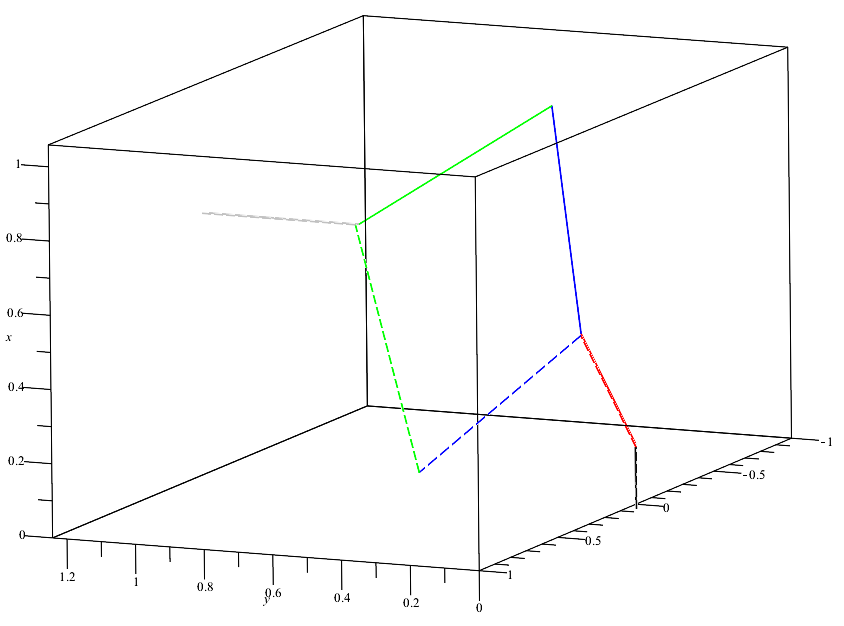
\includegraphics[width=0.80\textwidth]{figs/elbowupdown}
 	\caption{Exemplo de duas soluções possíveis para o mesmo ponto}
 	\label{fig::elbowupdown}
\end{figure}


\subsubsection{Cálculo da orientação da ferramenta}

Nesta etapa, deseja-se calcular a orientação da ferramenta, em relação ao
referencial inercial. Para isso são utilizados os ângulos $\phi,\theta,\psi$
para reresentar os ângulos de Euler das 3 rotações que orientam o referencial do
pulso na direção desejada.

Recorrendo novamente ao desenvolvimento da cinemática inversa geral para este
tipo de manipulador, da seção~\ref{sec::ikin}, obteve-se da
equação~\ref{eq::rut} a relação:
%
\begin{equation*}
	R_{U}^{T} = (R_{Z}^{U})^T R_{yzy}
\end{equation*}
%
Onde $R_{zyz}$ representa a matriz rotação pelos ângulos de Euler
$\phi,\theta,\psi$, em torno dos eixos $Y,Z,Y$ respectivamente.

As matrizes de rotação $(R_{Z}^{U})^T$ e $R_{U}^{T}$ são calculadas para os
valores de $q_1, q_2$ e $q_3$ das equações~\ref{eq::q1ik} a \ref{eq::q3ik}.
Assim, a equação~\ref{eq::rut} fornece um sistema de 9 equações e 6
incógnitas, se consideradas as funções senos e cossenos de $q_4, q_5$ e $q_6$ a serem
determinadas.
%
\begin{multline} \label{eq::rut}
%eq1
	 \left( \begin {array}{ccc} {\it c4}\,{\it c5}\,{\it c6}-{\it s4}\,{
\it s6}&-{\it c4}\,{\it s5}&{\it c4}\,{\it c5}\,{\it s6}+{\it c6}\,{
\it s4}\\ \noalign{\medskip}{\it s5}\,{\it c6}&{\it c5}&{\it s5}\,{
\it s6}\\ \noalign{\medskip}-{\it c5}\,{\it c6}\,{\it s4}-{\it c4}\,{
\it s6}&{\it s4}\,{\it s5}&-{\it c5}\,{\it s4}\,{\it s6}+{\it c4}\,{
\it c6}\end {array} \right) = \\
%eq2
	 \left( \begin {array}{ccc} {\it c2}\,{\it c3}-{\it s2}\,{\it s3}&-{
\it c2}\,{\it s3}-{\it s2}\,{\it c3}&0\\ \noalign{\medskip}{\it c1}\,{
\it c2}\,{\it s3}+{\it c1}\,{\it s2}\,{\it c3}&{\it c1}\,{\it c2}\,{
\it c3}-{\it c1}\,{\it s2}\,{\it s3}&-{\it s1}\\ \noalign{\medskip}{
\it s1}\,{\it c2}\,{\it s3}+{\it s1}\,{\it s2}\,{\it c3}&{\it s1}\,{
\it c2}\,{\it c3}-{\it s1}\,{\it s2}\,{\it s3}&{\it c1}\end {array}
 \right)^T \cdot \\
%eq3
	\cdot \left( \begin {array}{ccc} c\phi \,c\theta \,c\psi -s\phi \,s\psi &-c
\phi \,s\theta &c\phi \,c\theta \,s\psi +s\phi \,c\psi 
\\ \noalign{\medskip}s\theta \,c\psi &c\theta &s\theta \,s\psi 
\\ \noalign{\medskip}-s\phi \,c\theta \,c\psi -c\phi \,s\psi &s\phi \,
s\theta &-s\phi \,c\theta \,s\psi +c\phi \,c\psi \end {array} \right) 
\end{multline}
%

Analisando o lado esquerdo da equação~\ref{eq::rut} pode-se determinar
facilmente a solução para $\cos(q5)$, porque este será diretamente o resultado
alocado no termo $[2,2]$ da matriz $3 \times 3$ resultante do lado direito da
equação, ou seja:
%
\begin{multline}
\cos(q5) = {\it c2}\,{\it c3}\,s\phi \,{\it s1}\,s\theta -s\phi \,{\it s1}\,{\it 
		s2}\,{\it s3}\,s\theta +c\phi \,{\it c2}\,{\it s3}\,s\theta +
		\\ +c\phi \,{\it c3}\,{\it s2}\,s\theta +{\it c1}\,{\it c2}\,{\it c3}\,c\theta -{
		\it c1}\,{\it s2}\,{\it s3}\,c\theta 
\end{multline}
%
E seu seno é calculado por:
%
\begin{equation}
	\sin(q5) = \sqrt{1-\cos(q5)^2}
\end{equation}
%
Logo, utilizando a relação trigonométrica, $\sin(q5)/\cos(q5) = \tan(q5)$,
e invertendo a função tangente, determina-se:
%
\begin{equation}
	q5 = \atantwo(\sqrt{1-\cos(q5)^2}, \cos(q5))
\end{equation}
%

Para determinar $q4$ analisa-se novamente a matriz $R_{U}^{T}$. Se dividir o
termo $[3,2]$,  multiplicado por $(-1)$, pelo termo $[1,2]$, dos lados esquerdo
e direito da equação~\ref{eq::rut}, obtém-se uma expressão para $\tan(q4)$.
Invertendo a função tangente para obter $q4$:
\begin{multline} 
q4 = \atantwo( {{\it c1}\,s\phi \,s\theta -{\it s1}\,c\theta} , ~
 \left[  \left( s\phi \,{\it s1}\,{\it s3}-c\phi \,{\it c3} \right) {
\it c2}+{\it s2}\, \left( {\it c3}\,s\phi \,{\it s1}+c\phi \,{\it s3}
 \right)  \right] s\theta +
 \\ +{\it c1}\,c\theta \, \left( {\it c2}\,{\it 
s3}+{\it s2}\,{\it c3} \right) 
 )
\end{multline}
%
Similarmente à solução de $q4$, mas desta vez fazendo a divisão dos termos
$[2,3]$ por $[2,1]$, dos lados esquerdo e direito da equação~\ref{eq::rut},
encontra-se $q6$:
%
\begin{equation} \label{eq::q6ik}
	q6 = \atantwo ( {s6} , {c6} )
\end{equation}
%
Onde:
%
\begin{multline*}
	s6 = -{\it c2}\,{\it c3}\,s\phi \,s\psi \,{\it s1}\,c\theta +s\phi \,s\psi 
		\,{\it s1}\,{\it s2}\,{\it s3}\,c\theta +c\phi \,c\psi \,{\it c2}\,{
		\it c3}\,{\it s1}-c\phi \,c\psi \,{\it s1}\,{\it s2}\,{\it s3} +
		\\ -c\phi \,{\it c2}\,s\psi \,{\it s3}\,c\theta -c\phi \,{\it c3}\,s\psi \,{\it 
		s2}\,c\theta +{\it c1}\,{\it c2}\,{\it c3}\,s\psi \,s\theta -{\it c1}
		\,s\psi \,{\it s2}\,{\it s3}\,s\theta +
		\\ -c\psi \,{\it c2}\,s\phi \,{\it s3}-c\psi \,{\it c3}\,s\phi \,{\it s2}
\end{multline*}
\vspace{-15mm}
\begin{multline*}
	c6 = -c\psi \,{\it c2}\,{\it c3}\,s\phi \,{\it s1}\,c\theta +c\psi \,s\phi 
		\,{\it s1}\,{\it s2}\,{\it s3}\,c\theta -c\phi \,c\psi \,{\it c2}\,{
		\it s3}\,c\theta -c\phi \,c\psi \,{\it c3}\,{\it s2}\,c\theta 
		\\ -c\phi \,{\it c2}\,{\it c3}\,s\psi \,{\it s1}+c\phi \,s\psi \,{\it s1}\,{\it 
		s2}\,{\it s3}+c\psi \,{\it c1}\,{\it c2}\,{\it c3}\,s\theta -c\psi \,{
		\it c1}\,{\it s2}\,{\it s3}\,s\theta +
		\\ +{\it c2}\,s\phi \,s\psi \,{\it s3}+{\it c3}\,s\phi \,s\psi \,{\it s2}
\end{multline*}
%
Com o cálculo dos ângulos $q4, q5$ e $q6$ é possível determinar totalmente a
posição da ponta da ferramenta, pela equação~\ref{eq::posf}.
Como este ponto está alinhado ao eixo do efetuador, faz-se $dx = dz = 0$ e $dy
= pBTy$.
Reescrevendo a equação no referencial inercial, as componentes do vetor
$^{Z}\mathbf{p}_{f}$ são:
%
\begin{multline}
	x_f =  \left[  \left( -{\it c4}\,{\it s5}\,{\it pBTy}+{\it pURx} \right) {
		\it c3}+ \left( -{\it c5}\,{\it pBTy}-{\it pURy} \right) {\it s3}+{
		\it pLUx} \right] {\it c2} +
		\\ -{\it s2}\, \left( {\it c5}\,{\it pBTy}+{
		\it pURy} \right) {\it c3}+{\it s3}\, \left( {\it c4}\,{\it s5}\,{\it 
		pBTy}-{\it pURx} \right) {\it s2}+
		\\ +{\it pZSx}+{\it pSLx}
\end{multline}
\vspace{-15mm}
\begin{multline}
	y_f =  \{ \left[  \left( -{\it c4}\,{\it s5}\,{\it pBTy}+{\it pURx}
 		\right) {\it c3}+ \left( -{\it c5}\,{\it pBTy}-{\it pURy} \right) {
		\it s3}+{\it pLUx} \right] {\it s2}+ 
		\\ + \left[  \left( {\it c5}\,{\it 
		pBTy}+{\it pURy} \right) {\it c3}-{\it s3}\, \left( {\it c4}\,{\it s5}
		\,{\it pBTy}-{\it pURx} \right)  \right] {\it c2}+{\it pSLy} \} {
		\it c1} +
		\\ -{\it s5}\,{\it s1}\,{\it s4}\,{\it pBTy}
\end{multline}
\vspace{-15mm}
\begin{multline}
	z_f =  \{  \left[ \left( -{\it c4}\,{\it s5}\,{\it pBTy}+{\it pURx}
 		\right) {\it c3}+ \left( -{\it c5}\,{\it pBTy}-{\it pURy} \right) {
		\it s3}+{\it pLUx} \right] {\it s2}+ 
		\\ + \left[ \left( {\it c5}\,{\it 
		pBTy}+{\it pURy} \right) {\it c3}-{\it s3}\, \left( {\it c4}\,{\it s5}
		\,{\it pBTy}-{\it pURx} \right)  \right] {\it c2}+{\it pSLy} \} {
		\it s1} +
		\\ +{\it c1}\,{\it s4}\,{\it s5}\,{\it pBTy}
\end{multline}



Tem-se portanto, pelo conjunto de equações~\ref{eq::q3ik} a \ref{eq::q6ik}, a
solução cinemática inversa do manipulador MOTOMAN MH12.


\subsection{Tarefa e trajetória} \label{sec::tarefa_traj}

As trajetórias para representar este processo serão simplificadas neste
trabalho, pela consideração de que as superfícies são planas e que pode-se
representar a trajetória totalmente naquele plano.

A trajetória será modelada por um conjunto de funções de referência no tempo,
para cada coordenada generalizada. Como o planejamento é feito pela função da
posição da ferramenta no tempo, são utilizadas as soluções da cinemática
inversa, desenvolvidadas na seção anterior.

É claro que dependendo da posição e orientação da superfície a ser coberta pelo
robô, este assumirá diferentes configurações, que causam excitações diferentes
em sua base. Na seção~\ref{sec::casos}, dois casos de trajetória para
revestimento são analisados, com o objetivo de verificar os efeitos também da
trajetória nos erros devido a dinâmica do sistema robô-base. 

Para exemplificar os conceitos abordados nesta seção, considere-se a seguinte
tarefa para cálculo da trajetória:
%
\newline
\begin{tcolorbox}
[colframe=black!75!white, colback=white, title = Trajetória -- Exemplo] 
  \textbf{Tarefa:} Revestimento por HVOF \\
  \textbf{Área:} $(600 \times 300)~mm^2$ \\
  \textbf{Ponto inicial:} $\mathbf{p}_f = [0,700,~1,238,~-0,600]^Z$ \\
  \textbf{Orientação:} $\boldsymbol{\Phi}_{f} = [0,~0,~0]^Z$ \\
  \textbf{Passo:} $10~mm$ \\
  \textbf{Número de paralelos:} 50 \\
  \textbf{Velocidade da ferramenta:} $40~m/min$
\end{tcolorbox}
%
De acordo com o exemplo, a orientação do plano da superfície,
está alinhado ao sistema de coordenadas inercial e paralelo ao plano $xz$. A
Figura~\ref{fig::trajec_600x500x10} apresenta os 50 paralelos da trajetória ao
longo desta região.

\begin{figure}[h]
	\centering 
 	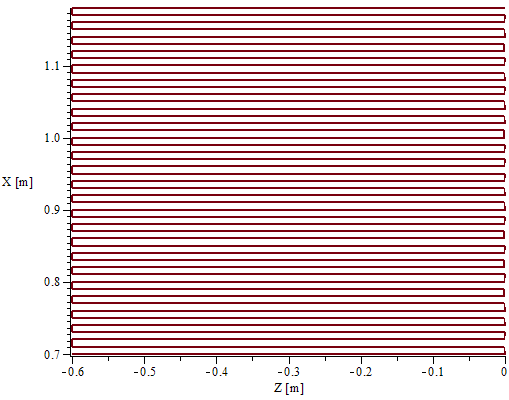
\includegraphics[width=0.60\textwidth]{figs/trajec_600x500x10}
 	\caption{Exemplo da trajetória de revestimento de uma região}
 	\label{fig::trajec_600x500x10}
\end{figure}

A Figura~\ref{fig::trajec3D_600x500x10} apresenta essa tarefa no ambiente 3D
de simulação, com o robô no início da trajetória.

\begin{figure}[h!]
	\centering 
 	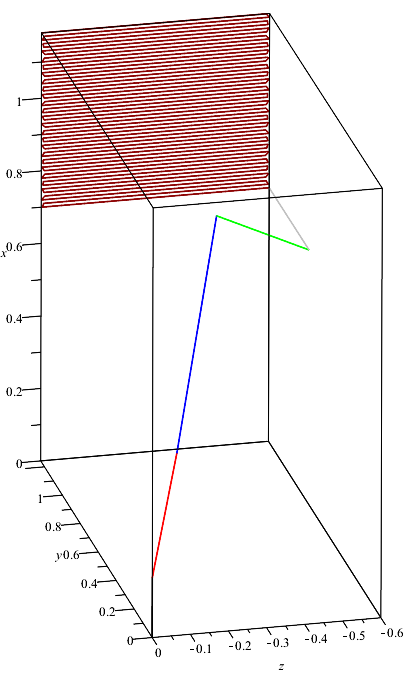
\includegraphics[width=0.50\textwidth]{figs/trajec3D_600x500x10}
 	\caption{Trajetória no ambiente 3D}
 	\label{fig::trajec3D_600x500x10}
\end{figure}

\subsubsection{Caminho ponto-a-ponto e função da trajetória}

O objetivo é determinar a função da trajetória em que robô realiza a tarefa de
revestimento. Primeiramente, define-se o conjunto ponto-a-ponto que forma o
caminho. A função temporal que liga os pontos do caminho é a trajetória.

Os pontos serão definidos nos vértices em que há mudança de direção da
ferramenta, ou seja, no início e fim de cada paralelo. Cada ponto será descrito
pela sua posição no ambiente em função do tempo. Logo:
%
\begin{equation} \label{eq::posi}
	\mathbf{p}_i = [~ px_{i}(t),~ py_{i}(t),~ pz_{i}(t)~]^Z
\end{equation}
%
Deseja-se que a velocidade da ferramenta entre os pontos seja controlada pelo
PID. Então, é preciso que a derivada da função trajetória entre os pontos seja a
velocidade desejada. Logo, a função da trajetória entre dois pontos de um mesmo
paralelo pode ser escrita como:
%
\begin{equation} \label{eq::pi}
\begin{split}
	p_i & = p_{i-1} + v \cdot \Delta t \\
		& = p_{i-1} + v \cdot (t-t_{i-1})
\end{split}
\end{equation}
%
Onde $v$ é a velocidade da ferramenta do ponto $p_{i-1}$ a $p_{i}$ e
$\Delta t$ é a variação de tempo entre o instante $t$ e o valor do tempo no
início da trajetória naquele paralelo $t_{i-1}$. A velocidade considerada neste
exemplo é de $40~m/min$.

Pode-se então calcular o intervalo de tempo entre cada ponto do caminho por:
%
\begin{equation} \label{eq::dt}
	\Delta t = \frac{p_i - p_{i-1}}{v}
\end{equation}
%
Portanto, o tempo associado a cada ponto do caminho é determinado por:
%
\begin{equation} \label{eq::ti}
	t_i = t_{i-1} + \Delta t
\end{equation}
%
Com as equações~\ref{eq::pi} e \ref{eq::ti}, define-se a função da trajetória
para cada paralelo.
%
\begin{table}[h]
\centering
\caption{Resumo dos pontos e funções trajetória do exemplo}
\label{tab::func_paralelos}
\begin{tabular}{|c|c|c|c|c||c|c|c|}
\hline
i & $px_i$ & $py_i$ & $pz_i$ & $t_i$  & $px_i(t)$    & $py_i(t)$ &
$pz_i(t)$
\\ \hline \hline
1       & 0,70  & 0,8   & -0,6  & 1,000 & 0,7         & 0,8      & -0,6         \\ \hline
2       & 0,70  & 0,8   & 0     & 1,900 & 0,7         & 0,8      & -1,27+0,67t  \\ \hline
3       & 0,71  & 0,8   & 0     & 1,915 & -0,57+0,67t & 0,8      & 0            \\ \hline
4       & 0,71  & 0,8   & -0,6  & 2,815 & 0           & 0,8      & 1,27-0,67t   \\ \hline
5       & 0,72  & 0,8   & -0,6  & 2,830 & -1.167+.67t & 0,8      & -0,6         \\ \hline
6       & 0,72  & 0,8   & 0     & 3,730 & 0,72        & 0,8      & -2,487+0,67t \\ \hline
7       & 0,73  & 0,8   & 0     & 3,745 & -1,77+0,67t & 0,8      & 0            \\ \hline
8       & 0,73  & 0,8   & -0,6  & 4,645 & 0,73        & 0,8      & 2,497-0,67t  \\ \hline
\end{tabular}
\end{table}
%

A Tabela~\ref{tab::func_paralelos} apresenta os termos do vetor posição da
equação~\ref{eq::posi} e as funções trajetória para os primeiros 4 paralelos do
exemplo. A Figura~\ref{fig::pontos_exemplo} ilustra os pontos indicados na
tabela no gráfico da trajetória.

\begin{figure}
	\centering 
 	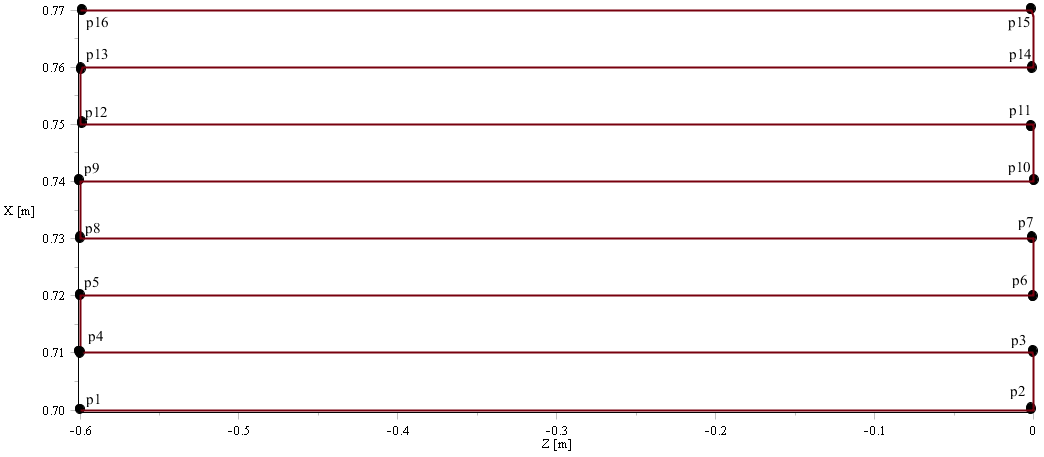
\includegraphics[width=0.90\textwidth]{figs/pontos_exemplo}
 	\caption{Os pontos do caminho dos 8 primeiros paralelos}
 	\label{fig::pontos_exemplo}
\end{figure}

\subsubsection{\textit{Piecewise function} e cinemática inversa}

As funções $px_i(t), py_i(t)$ e $pz_i(t)$, podem ser tratadas como uma única
função, através do uso do comando \texttt{piecewise}, no Maple. Os argumentos
deste comando são simplesmente as funções contidas em cada intervalo de tempo,
resultando em uma função única, dividida por partes, sem necessidade de serem
contínuas. A vantagem é que essas funções podem ser derivadas, sendo reconhecido
que na discontiuidade a função é indefinida.
Outra vantagem é que pode ser utilizada diretamente para calcular, por meio da
cinemática inversa, as funções das coordenadas generalizadas que descrevem o
conjunto de posições, para todo o intervalo de tempo.

No Maple, a função \textit{piecewise} resultante tem a seguinte forma:
%
\begin{equation}
p_{piecewise} = 
\begin{cases}
p0 & t<t1 \\
p1 & t<t2 \\
p2 & t<t3 \\
p3 & t<t4 \\
p4 & otherwise
\end{cases}
\end{equation}
%

Pelas equações~\ref{eq::q3ik} a \ref{eq::q6ik} foram definidas as coordenadas
generalizadas $q1$ a $q6$ em funcão da posição da ferramenta, $^Z\mathbf{p}_f$.
Logo, basta substituir a função \textit{piecewise} de cada termo de
$^Z\mathbf{p}_f$ em $q1$ a $q6$ para obter o resultado da cinemática inversa por
partes, ou intervalos de tempo.

Esta nova função será utilizada como parâmetro de entrada no modelo dinâmico,
para as coordenadas de referência $q_1ref$ a $q_5ref$. Isso faz com que o
controle PID forneça os torques para atingir estas coordenadas ao
longo do tempo e assim perseguir a trajetória determinada. A
Figura~\ref{fig::res_exemplo} apresenta o gráfico do resultado da cinemética
inversa utilizando as função \textit{piecewise} para a posição e velocidade da
ferramenta durante os primeiros 8 paralelos da tarefa. 

\begin{figure}[h]
    \centering
    \begin{subfigure}[b]{0.45\textwidth}
        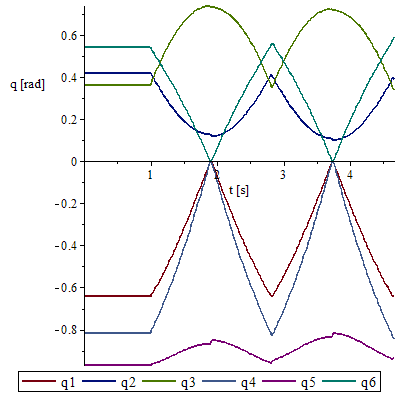
\includegraphics[width=\textwidth]{figs/qxt_exemplo}
        \caption{Resultado cinemático dos ângulos de referência }
        \label{fig::qxt_exemplo}
    \end{subfigure}
    \quad %add desired spacing between images, e. g. ~, \quad, \qquad, \hfill
    % etc.
      %(or a blank line to force the subfigure onto a new line)
    \begin{subfigure}[b]{0.45\textwidth}
        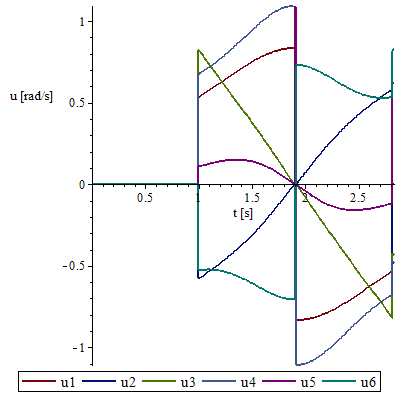
\includegraphics[width=\textwidth]{figs/uxt_exemplo}
        \caption{Resultado cinemático das velocidades de referência}
        \label{fig::uxt_exemplo}
    \end{subfigure}
    \caption{Resultados cinemáticos do exemplo de
    trajetória}\label{fig::res_exemplo}
\end{figure}


\subsection{Modelo teórico MBS -- Robô}

Nas seções anteriores foram desenvolvidas as equações simbólicas da
cinemática direta, cinemática inversa e dinâmica do manipulador robótico. 
Gerou-se portanto um modelo dinâmico (MBS) do robô, tal que é
possível realizar simulações de qualquer tarefa que se desejar. Para isso, são
listadas as seguintes etapas:

\begin{enumerate}
  \item Definir os sistemas de coordenadas locais dos elos do manipulador;
  \item Definir as coordenadas generalizadas do sistema;
  \item Fornecer os parâmetros de geometria e inércia do robô;
  \item Definir os parâmetros do controlador PID;
  \item Fornecer os requisitos da tarefa (no caso do revestimento: orientação,
  velocidade, passo);
  \item Definir os pontos do caminho a ser percorrido pela ferramenta, pela
  cinemática inversa;
  \item Calcular a trajetória e fornecer as coordenadas de referência no
  modelo dinâmico direto;
  \item Executar a simulação da tarefa. 
\end{enumerate}

Utiliza-se novamente o exemplo dado na seção~\ref{sec::tarefa_traj} para
demonstrar os resultados obtidos pelo modelo MBS. Dada a tarefa de revestimento
do exemplo, realiza-se a simulação do modelo dinâmico com os valores de
referência calculados pela cinemática inversa.  Os resultados apresentados
resumem-se apenas aos 4 primeiros paralelos, a fim de facilitar a visualização.

Este modelo MBS conta com uma animação do movimento do robô realizando a
trajetória, onde a posição da ferramenta deixa um rastro a partir do início da
trajetória planejada. A sequência de Figuras~\ref{fig::mbs3D_exemplo} fornece
alguns quadros da animação, em 4 instantes de tempo.

\begin{figure}[h]
    \centering
    \begin{subfigure}[b]{0.4\textwidth}
        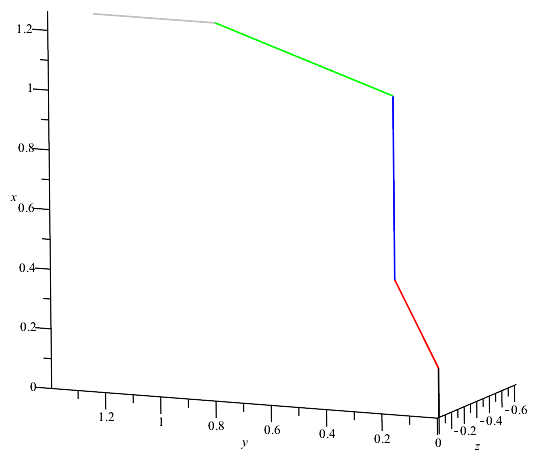
\includegraphics[width=\textwidth]{figs/mbs3D_0s}
        \caption{$0~s$}
        \label{fig::mbs3D_0s}
    \end{subfigure}
    \quad %add desired spacing between images, e. g. ~, \quad, \qquad, \hfill
    % etc.
      %(or a blank line to force the subfigure onto a new line)
    \begin{subfigure}[b]{0.4\textwidth}
        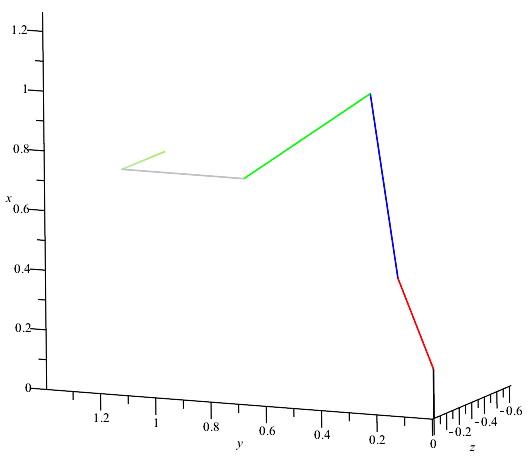
\includegraphics[width=\textwidth]{figs/mbs3D_1s5}
        \caption{$1,5~s$}
        \label{fig::mbs3D_1s5}
    \end{subfigure}
    \quad %add desired spacing between images, e. g. ~, \quad, \qquad, \hfill
    % etc.
      %(or a blank line to force the subfigure onto a new line)
    \begin{subfigure}[b]{0.4\textwidth}
        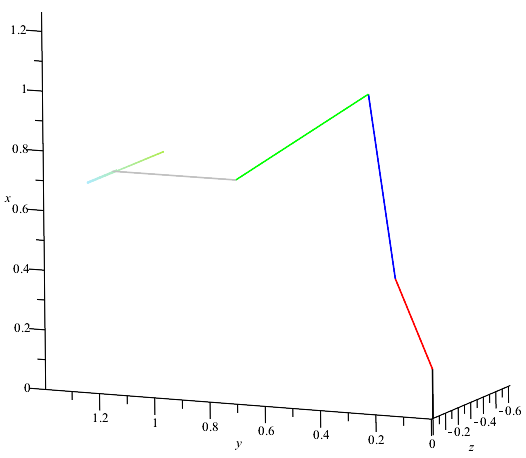
\includegraphics[width=\textwidth]{figs/mbs3D_2s5}
        \caption{$2,5~s$}
        \label{fig::mbs3D_2s5}
    \end{subfigure}
    \quad %add desired spacing between images, e. g. ~, \quad, \qquad, \hfill
    % etc.
      %(or a blank line to force the subfigure onto a new line)
    \begin{subfigure}[b]{0.4\textwidth}
        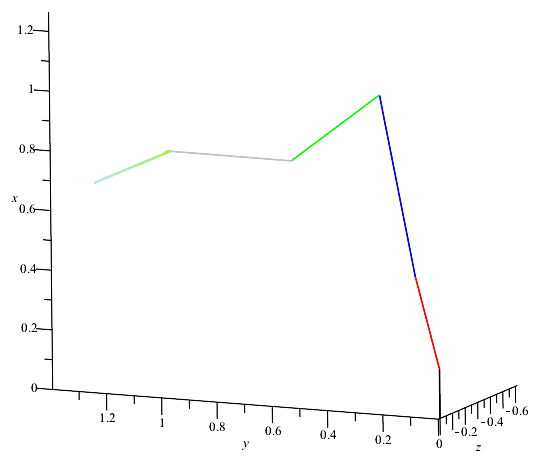
\includegraphics[width=\textwidth]{figs/mbs3D_3s}
        \caption{$3~s$}
        \label{fig::mbs3D_3s}
    \end{subfigure}
    \caption{Animação da trajetória no ambiente 3D} \label{fig::mbs3D_exemplo}
\end{figure}

O resultado seguinte compara a variação angular de referência das juntas, pela
cinemática inversa, e o efetivo, resultado do modelo dinâmico.
A Figura~\ref{fig::qxt_ex_realxideal} apresenta em linha pontilhada o valor dos
ângulos de referência, e em linha cheia, os efetivos.

\begin{figure}[h]
	\centering 
 	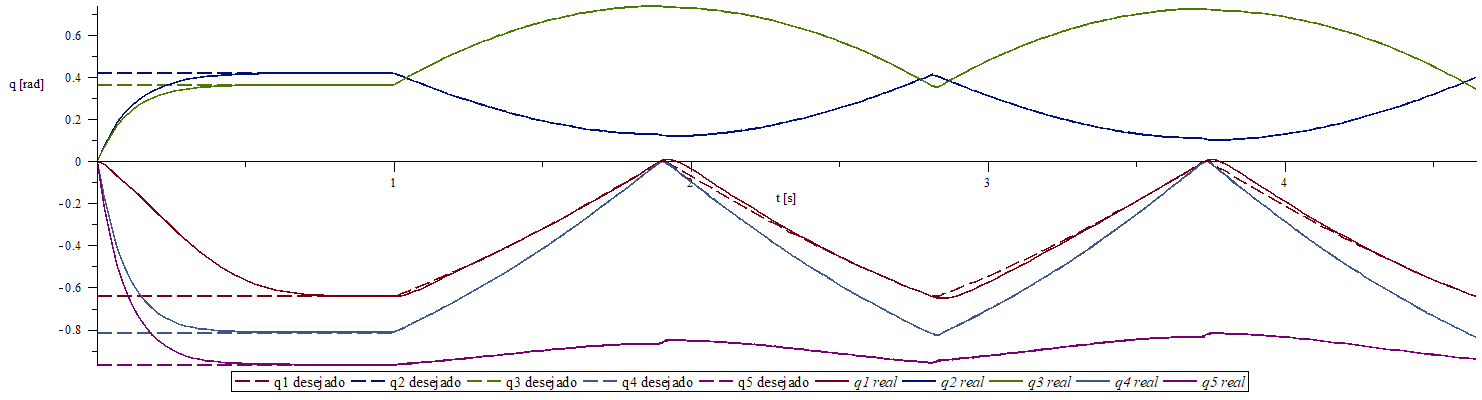
\includegraphics[width=0.75\textwidth]{figs/qxt_ex_realxideal}
 	\caption{Comparação referência x efetivo dos ângulos das juntas}
 	\label{fig::qxt_ex_realxideal}
\end{figure}

Compara-se também a posição efetiva da ferramenta, resultado da dinâmica, em
comparação com a posição esperada, do cálculo da cinemática inversa. Este
resultado é interessante porque fornece um parâmetro direto para avaliar o
efeito total da dinâmica do robô na posição final da ponta da ferramenta.
A Figura~\ref{fig::errop_exemplo} apresenta o resultado comparativo entre as
posições de referência e efetivas de cada coordenada $(x, y, z)$ do vetor
posição da ferramenta.

\begin{figure}[h]
	\centering 
 	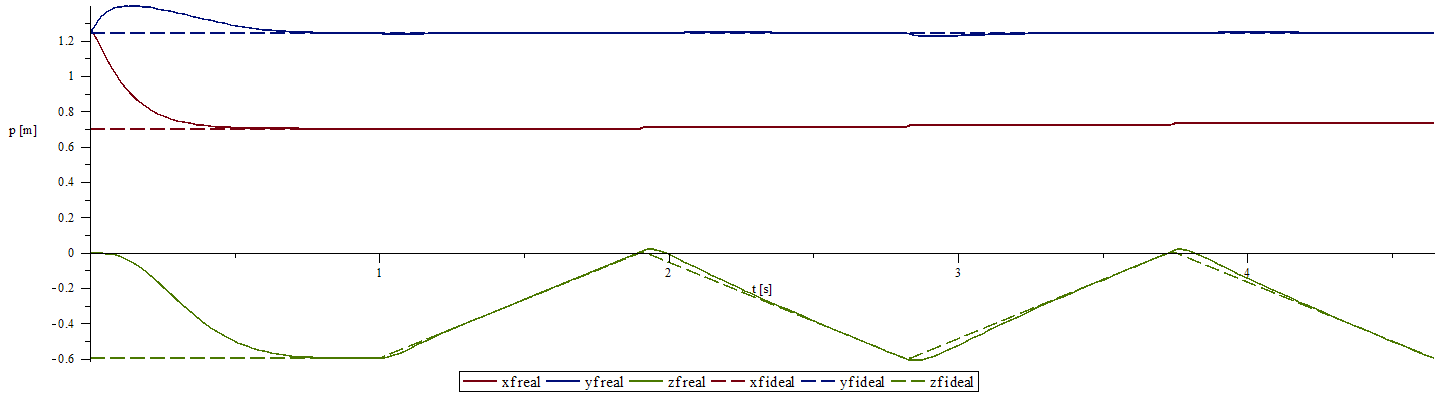
\includegraphics[width=0.75\textwidth]{figs/errop_exemplo}
 	\caption{Comparação referência x efetivo da posição da ferramenta}
 	\label{fig::errop_exemplo}
\end{figure}

Nota-se que neste modelo MBS o robô é capaz de seguir com boa precisão a
trajetória informada. Para facilitar a visualização, a
Figura~\ref{fig::erros_exemplo_z} apresenta um gráfico do erro de cada coordenada
da posição, ao longo da trajetória. A linha pontilhada representa o erro
absoluto, ou seja, a norma do erro em cada direção.

\begin{figure}[h]
	\centering 
 	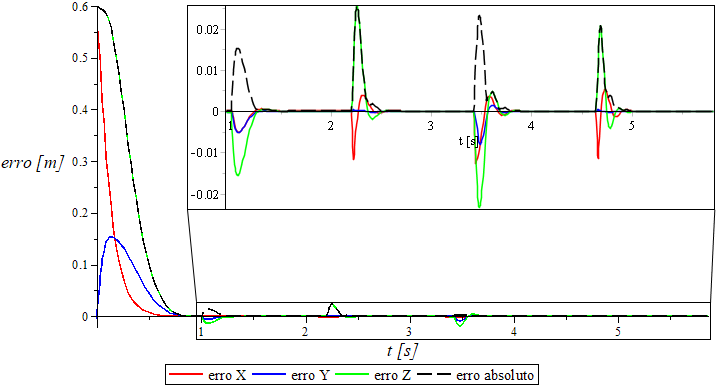
\includegraphics[width=0.90\textwidth]{figs/erros_exemplo_z}
 	\caption{Erro de posição da ferramante em cada direção}
 	\label{fig::erros_exemplo_z}
\end{figure}

Observa-se por este resultado que o erro de posicionamento, a partir do início
da região a ser revestida (em $t>1s$), é da ordem de $10^{-1}~mm$ durante
apriximadamente $70\%$ do caminho de um paralelo. Próximo ao início e fim dos
paralelos esse erro cresce devido ao transitório de direção e sentido do
deslocamento, que não são acompanhados perfeitamente pela dinâmica do robô.
Estes erros chegam a uma ordem de $20~mm$ nestas regiões.

Da mesma forma que foi feito para a posição, pode-se verificar os erros de
velocidade da ferramenta. Para isso, deriva-se a a posição da ferramenta, com
respeito ao tempo e obtém-se o vetor velocidade. O resultado de cada componente
e do valor absoluto do erro para a tarefa do exemplo é apresentado na
Figura~\ref{fig::errovel_exemplo}.

\begin{figure}[h]
	\centering 
 	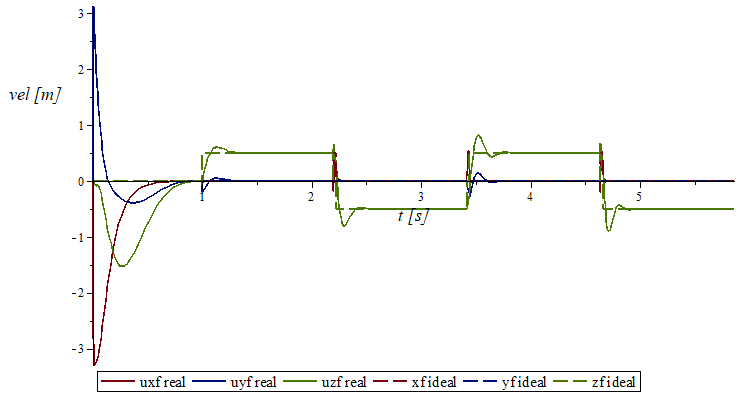
\includegraphics[width=0.90\textwidth]{figs/errovel_exemplo}
 	\caption{Erro de velocidade da ferramenta em cada direção}
 	\label{fig::errovel_exemplo}
\end{figure}

% Os erros tolerados variam de acordo com os critérios definidos na
% seção~\ref{sec::requisitos}\todo{Incluir seção com os requisitos do
% revestimento} e serão analisados mais detalhadamente na
% seção~\ref{sec::casos}.

Por último, calcula-se o erro de orientação, definido como a diferença entre a
orientação da superfície dada pela cinemática inversa, e a orientação resultante
da simulação dinâmica. 
É representada por uma matriz, determinada pela transformação homogênea entre o
referencial inercial, SC-Z, e o referencial localizado no pulso, SC-B, já que a
ferramenta é fixada neste último. Logo, pode-se comparar as duas matrizes, ideal
e efetiva, para cálculo do erro.

Como apresentado na seção~\ref{sec::cinematica} uma maneira mais prática de
representar o erro de orientação é por meio de um escalar, que representa o
ângulo de desvio da ferramenta entre o caso ideal e o efetivo, de acordo com a
equação~\ref{eq::ang_erro}.

% Isto pode ser feito levando em consideração que estas matrizes são
% formadas por vetores unitários dispostos nas colunas da matriz e formam uma
% base ortonormal.\todo{Incluir teorema que calcula o angulo entre as bases}.

Seja a orientação ideal representada pela matriz $Mi$, que é função dos 3
ângulos de Euler $\phi,~\theta$ e $\psi$, e a matriz resultante da dinâmica por
$Me$, função do resultado de $q1(t),\ldots,q5(t)$, calcula-se:
%
\begin{equation}
	R = Me(q(t))~Mi(\phi,\theta,\psi)^{-1}
\end{equation}
%
Aplicando $R$ à equação~\ref{eq::ang_erro}, calcula-se o ângulo de desvio entre
as duas matrizes.
Para a tarefa do exemplo, as matrizes $Me$ e $Mi$ e $R$ em, por exemplo,
$t=2~s$ são:
%
 \begin{gather*}
 % eq1
 Me = \left( \begin {array}{ccc}  0.99755& 0.0&- 0.069955
\\ \noalign{\medskip}- 0.00262& 0.99930&- 0.037325
\\ \noalign{\medskip} 0.069903& 0.037413& 0.99685\end {array} \right) \\
% eq2
 Mi =  \left( \begin {array}{ccc}  1~& 0~& 0~\\ \noalign{\medskip} 0~&
 1~& 0~\\ \noalign{\medskip} 0~& 0~& 1~\end {array} \right) \\
 % eq3
R =  \left( \begin {array}{ccc}  1.0&- 0.00000058757&- 0.0021389
\\ \noalign{\medskip}- 0.000079441& 0.99930&- 0.037415
\\ \noalign{\medskip} 0.0021374& 0.037415& 0.99930\end {array}
 \right)
\end{gather*}
%
Logo, o erro de orientação neste instante de tempo do exemplo é:
%
\begin{equation*}
	\theta_{erro}(t=2~s) = 0,0375~rad
\end{equation*}
%
E aplicando-se o erro angular na equação~\ref{eq::eixo_erro}, obtém-se o eixo de
revolução do desvio. O resultado em $t=2~s$ é:
%
\begin{equation}
	\omega(t=2~s) = [0,6312,~-0,1755,~-0,4278]^Z
\end{equation}
%


O resultado do desvio de orientação da ferramenta, durante toda a tarefa é
apresentado no gráfico da Figura~\ref{fig::orierro_exemplo_z}.

\begin{figure}[h]
	\centering 
 	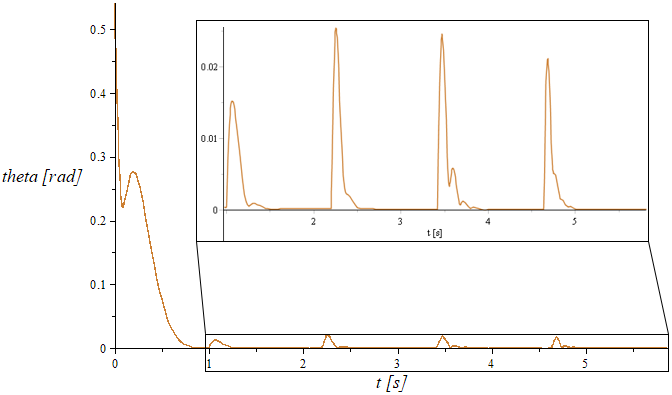
\includegraphics[width=0.85\textwidth]{figs/orierro_exemplo_z}
 	\caption{Erro de orientação da ferramenta}
 	\label{fig::orierro_exemplo_z}
\end{figure}

Note-se que não interessa o erro antes do manipulador iniciar a trajetória dos
paralelos do revestimento, ou seja, entre a posição inicial e o ponto p1
($t<1~s$), porque neste trecho manipulador não estaria realizando o
revestimento.
Analisando, portanto, o gráfico a partir de $1~s$ percebe-se um erro periódico,
devido às variações de direção, com amplitude máxima de aproximadamente
$0,038~rad$, ou $2,18^{\circ}$. 
% Apesar de não ser possível, apenas por este resultado escalar, afirmar a direção
% onde o erro é maior, pode-se comparar com o gráfico do erro de posicionamento,
% na Figura~\ref{fig::erros_exemplo}. É possível inferir que este erro está mais
% relacionado com o atraso do posicionamento na direção $z$ e portanto, grande
% parte do desvio de orientação está na direção vertical, $x$ de SC-Z.

Nesta seção foram explorados os resultados que simulações utilizando o modelo
MBS podem fornecer. Para isso, tomou-se como exemplo uma tarefa de cobertura de
uma superfície plana. Os métodos de cálculo dos erros de posicionamento,
velocidade e orientação da extremidade da ferramenta foram demonstrados e serão
utilizados para comparação de diferentes casos do modelo acoplado robô-base
flexível, realizando tarefas de revestimento de superfícies planas, que serão
propostos na seção~\ref{sec::casos}.



% -.~.-.~.-.~.-.~.-.~.-.~.-.~.-.~.-.~.-.~.-.~.-
\section{Modelo da base} \label{sec::base}

A base é definida, neste trabalho, como qualquer estrutura elástica, à qual o
manipulador robótico é fixado, que fornece flexibilidade devido às forças
dinâmicas exercidas pelo movimento do robô. A flexibilidade da estrutura causará
desvios do movimento esperado e controlado do robô e cabe ao método proposto
identificar e quantificar esses desvios e verificar se os requisitos do processo
serão satisfeitos. Para isso, é desenvolvido um modelo teórico da base, para ser
adicionado ao modelo do robô, formando o sistema MBS acoplado.

Nesta seção é demonstrado como uma estrutura construída com geometria,
materiais, restrições e infinitos graus de liberdade que seriam muito complexos
para serem descritos analiticamente em um modelo MBS, pode ser simplificado como
um sistema de massa-mola-amortecedor de 6 graus de liberdade.
Considera-se um conjunto de sistemas de coordenadas localizado no ponto teórico
onde é fixado o robô, na estrutura. A esse sistema, correspondem 3 movimentos de
translação $x,y,z$ e 3 movimentos de rotação $\theta_x, \theta_y, \theta_z$, que
formam as coordenadas generalizadas do modelo MBS.

Portanto, para realizar a simplificação é necessário obter uma matriz de rigidez
e uma matriz de amortecimento, associadas aos 6 gdl do corpo sobre a base. A
matriz de rigidez é obtida numericamente pela Análise por Elementos Finitos
(AEF) e a matriz de amortecimento pelo resultado experimental de análise modal,
detalhado na seção~\ref{sec::experimento}.

Por fim, desenvolve-se as equações que regem o movimento do corpo acoplado a
esse sistema massa-mola-amortecedor.
Foi utilizada a mesma metodologia do modelo do robô para desenvolvimento das
equações de movimento: pelo método de Kane e com uso das rotinas do programa
Sophia-Maple.

\subsection{Geometria e CAD}

A primeira etapa da modelagem da base é representar sua geometria em um modelo
CAD. Este modelo será utilizado para as simulações pela Análise por Elementos
Finitos, a fim de se obter sua matriz de rigidez.

Para ilustrar o método, será aproveitada a base projetada e construída para
testes do projeto EMMA. Consiste em uma estrutura metálica, formada por perfis
extrudados de alumínio estrutural. Sobre a estrutura um par de trilhos paralelos
permitem o movimento longitudinal da placa onde é fixado o robô. As dimensões
principais são 2 metros de comprimento, 0,8 metros de largura e 0,6 metros de
altura. A Figura~\ref{fig::estrut_modelo_fisico} apresenta uma fotografia da
base de testes.

\begin{figure}[h]
	\centering 
 	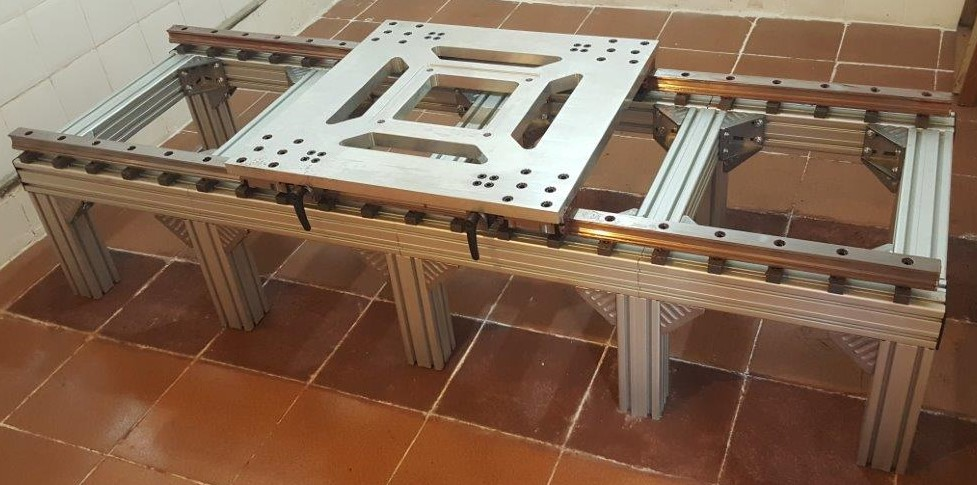
\includegraphics[width=0.70\textwidth]{figs/estrut_modelo_fisico}
 	\caption{Base de testes do robô}
 	\label{fig::estrut_modelo_fisico}
\end{figure}

O projeto desta base foi desenvolvido no programa SolidWorks, onde de forma
bastante detalhada, são incluídos os desenhos das peças customizadas, peças
comerciais, acessórios de união e fixadores mecânicos que compõe a montagem CAD
da estrutura. Este modelo é apresentado na Figura~\ref{fig::estrutCAD}, com os
principais componentes indicados, inclusive o robô.

\begin{figure}[h]
	\centering 
 	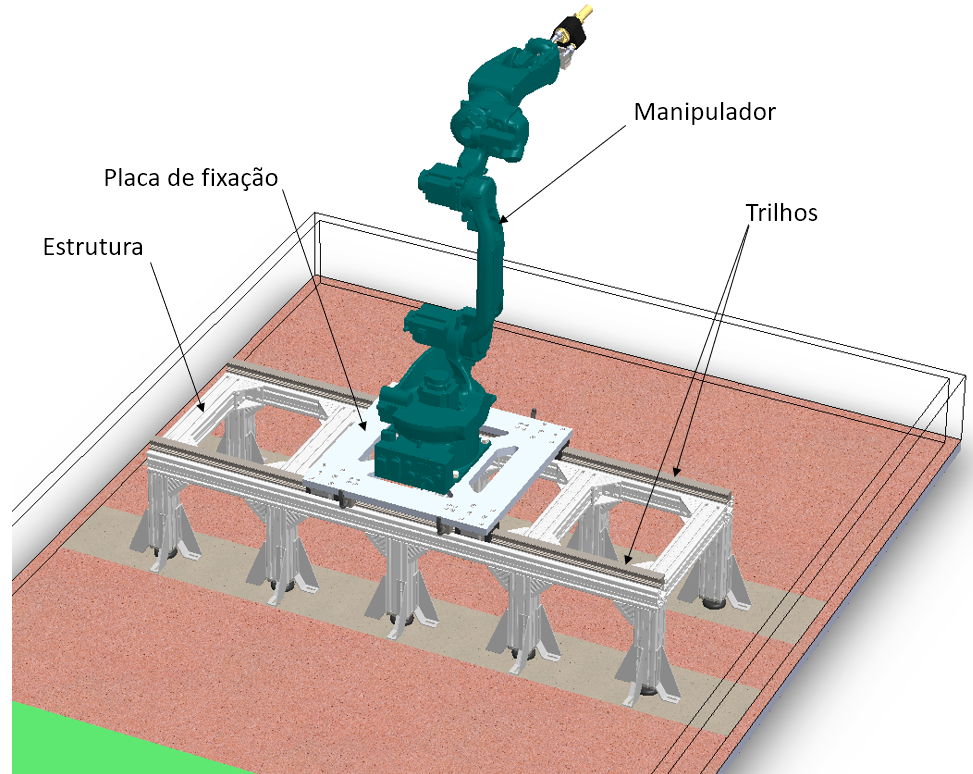
\includegraphics[width=0.75\textwidth]{figs/estrutCAD}
 	\caption{Modelo CAD detalhado da base e robô}
 	\label{fig::estrutCAD}
\end{figure}

O modelo CAD completo poderia ser diretamente utilizado nas
simulações para obtenção da matriz de rigidez desta estrutura. No entanto, o
alto nível de detalhamento dos componentes, além dos diversos contatos e
restrições entre as peças, requer um modelo de malha muito densa, não linear e
maior poder computacional. E o resultado teria muito informações irrelevantes
para esta análise, como por exemplo, tensões em elementos de fixação ou
deformação do rolamento do trilho.

Logo, o objetivo da simplificação é obter apenas os resultados que importam
na análise, e ignorar outros efeitos que não alteram significativamente
estes resultados. 

Para o modelo da base de testes, foram utilizados elementos unidimensionais, de
viga, para formar a estrutura e os trilhos. A união entre esses componentes foi
feita por elementos rígidos, representando os parafusos de fixação do trilho na
estrutura. A placa de fixação do robô foi representada também por elementos
unidimensionais rígidos, assumindo-se que sua rigidez é muito superior à rigidez
da estrutura, e o ponto de fixação do robô está localizado no centro desta
placa.
Os rolamentos do trilho foram substituídos por uma conexão rígida entre a placa
e os trilhos. Assim, a flexibilidade desta estrutura, no modelo simplificado
depende apenas das deformações dos elementos de viga que representam o trilho e
a estrutura. A Figura~\ref{fig::estrutFEA} apresenta o modelo simplificado para
a AEF, desenvolvida no programa Autodesk Simulation Mechanical.

\begin{figure}[h]
	\centering 
 	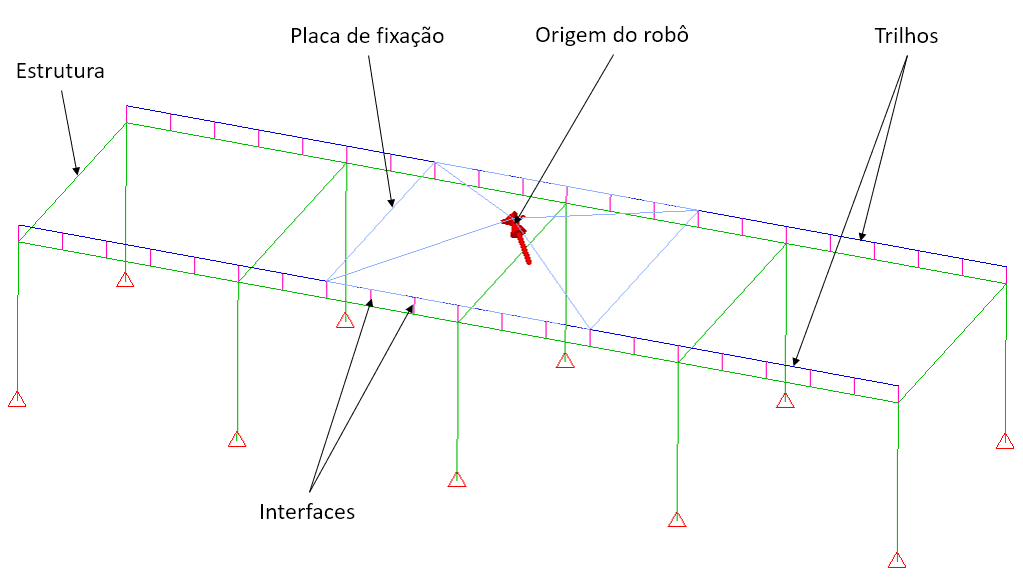
\includegraphics[width=0.75\textwidth]{figs/estrutFEA}
 	\caption{Modelo da base para AEF}
 	\label{fig::estrutFEA}
\end{figure}

\subsection{Análise por Elementos Finitos} \label{sec::aef}

Foi demonstrado na seção~\ref{sec::rigidez} um método analítico e sistemático
para obter a matriz de rigidez de uma estrutura em qualquer ponto de
interesse. Para estruturas simples, com poucos graus de liberdade e poucos
elementos, o método analítico se mostra bastante prático. Já para estruturas
mais complexas, com muitos elementos, conexões, restrições, graus de liberdade
e não linearidades, resolver pelo método analítico pode ser impraticável ou
desgastante.

Como deseja-se a rigidez da estrutura para apenas um ponto de interesse -- o
ponto onde virtualmente está fixado o robô -- propõe-se uma forma de, utilizando
os conceitos do método apresentado e simulações por AEF, extrair a matriz de
rigidez para este ponto. As simulações realizadas são do tipo lineares e
estáticas. A seguir são detalhadas as etapas para definir o modelo para AEF.

\subsubsection{Partes, elementos e propriedades}

O modelo é divido em estrutura, trilho, interfaces e placa, como foi ilustrado
na Figura~\ref{fig::estrutFEA} Para cada parte são definidos o tipo de elemento,
suas propriedades e material.

A estrutura é formada por perfis de alumínio estrutural. Esta é modelada como
elementos unidimensionais de viga. Isso significa que suas propriedades são
uniformes ao longo de apenas uma dimensão em todo o elemento, bastando fornecer
apenas suas propriedades de seção transversal. A
Figura~\ref{fig::sectrans_bosch} mostra o corte de seção de um elemento da
estrutura e suas propriedades. O material do perfil da estrutura é o Alumínio
EN-AW-6060. e as propriedades são incluidas no modelo, de acordo com a
Tabela~\ref{tab::prop_mat}.

\begin{figure}[h]
	\centering 
 	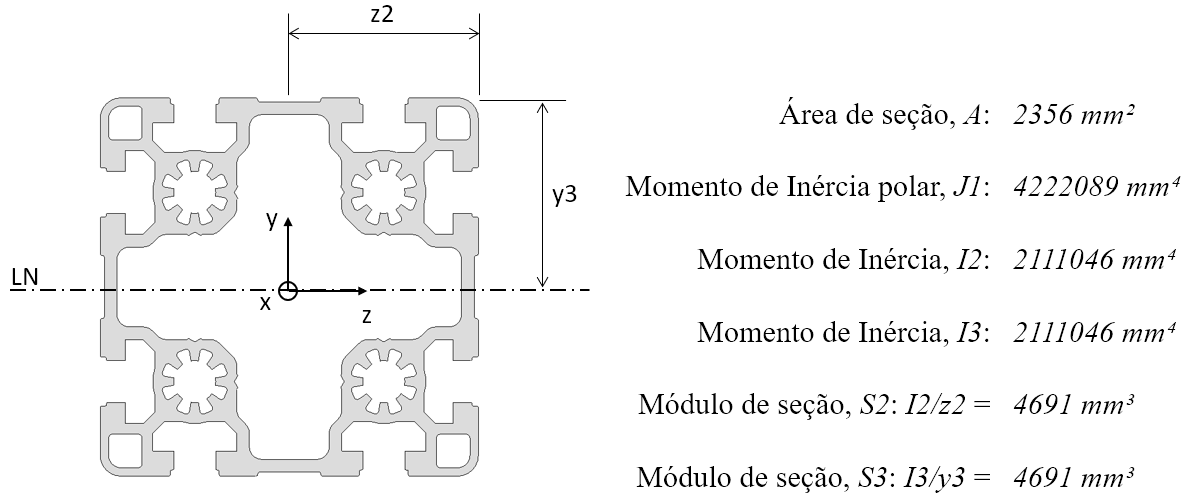
\includegraphics[width=0.90\textwidth]{figs/sectrans_bosch}
 	\caption{Seção transversal do elemento da estrutura}
 	\label{fig::sectrans_bosch}
\end{figure}

\begin{table}
\centering
\caption{Propriedades mecânicas dos materiais do modelo AEF}
\label{tab::prop_mat}
\begin{tabular}{@{}llcc@{}}
\toprule
\textbf{Propriedade}   &             & \textbf{EN-AW 6060} & \textbf{AISI 316} \\ \midrule
Densidade              & {[}g/cc{]}  & 2,70                & 7,90             \\
Módulo de Elasticidade & {[}GPa{]}   & 69,5                & 200               \\
Coeficiente de Poisson & {[}1{]}     & 0,34                & 0,29    			\\
Tensão de escoamento   & {[}MPa{]}   & 150                 & 240               \\
Resistência à tração   & {[}MPa{]}   & 150                 & 580               \\ \bottomrule
\end{tabular}
\end{table}

O trilho também é modelado como elemento de viga. Sua seção transversal e
propriedades estão na Figura~\ref{fig::sectran_trilho}. Seu material é o aço
carbono inoxidável AISI 316 e suas propriedades mecânicas estão na
Tabela~\ref{tab::prop_mat}.

\begin{figure}[h]
	\centering 
 	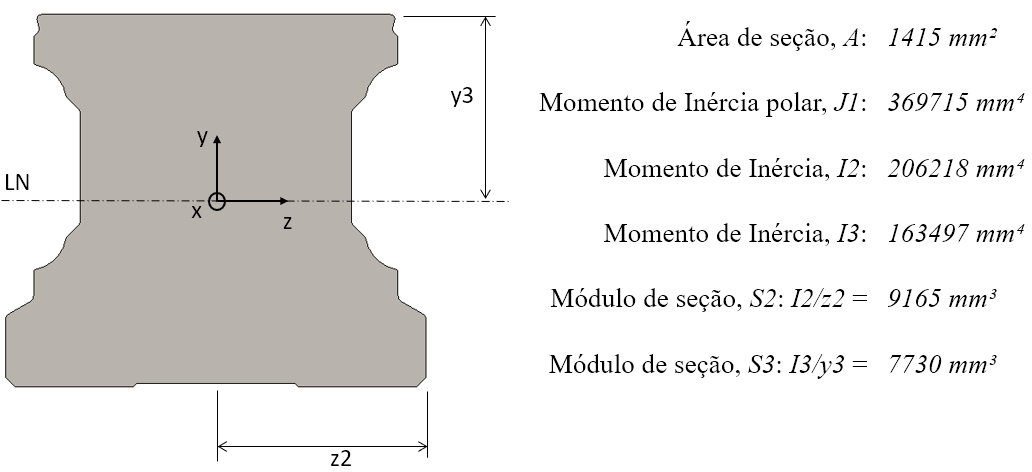
\includegraphics[width=0.90\textwidth]{figs/sectran_trilho}
 	\caption{Seção transversal do elemento do trilho}
 	\label{fig::sectran_trilho}
\end{figure}

As partes interface e placa de fixação do robô são modelados como elementos
unidimensionais rígidos, ou seja, transmitem apenas forças e momentos, mas não
se deformam. Ao todo são 40 peças de interface representando os 20 parafusos de
fixação de cada trilho. Já a placa de fixação é formada por um quadro de
elementos ligando os dois trilhos e uma ``pirâmide'' convergindo para o ponto de
fixação do robô. Como este ponto representa a conexão entre a estrutura e o
robô, aplica-se os esforços na estrutura diretamente neste. Os elementos
rígidos transmitem estes esforços ao trilho e à estrtura, e obtém-se os
resultado de forças de reação e deslocamentos resultantes.


\subsubsection{Restrições e conexões}

A base de testes é originalmente fixa no piso por meio de parafusos chumbadores.
Cada perna da estrurtura posssui 3 parafusos. No modelo AEF, esta restrição é
modelada como fixa, ou seja, não permite-se nenhuma translação ou rotação, e
é aplicada à extremidade inferior de cada perna.

Os elementos de cada parte são conectados por uniões ``soldadas'', ou seja, não
permitem nenhum grau de liberdade na extremidade do elemento onde há a conexão.


\subsubsection{Casos de Carregamento}

Para obter a matriz de rigidez, deve-se realiza-se ao todo 6 casos de
carregamento e restrições. Cada caso obtém 6 dos 36 termos, que correspondem a uma linha
da matriz $6 \times 6$. Os carregamentos e restrições são aplicados ao ponto
virtual de fixação do robô.

A cada caso é aplicado um deslocamento prescrito em uma direção. Às outras
direções são aplicadas restrições à translação e à rotação. Logo, um
deslocamento unitário na direção $x$ ($ux = 1~mm$), por exemplo, provoca uma
força ou momento de reação em todas as direções, no ponto virtual. A força de
reação correspondente à direção $x$ produz o termo de rigidez $k_{11}$, à
direção $y$, $k_{12}$, à direção $z$, $k_{13}$, e assim por diante. Este método
é uma versão para AEF do método analítico apresentado na
seção~\ref{sec::rigidez}. A Tabela~\ref{tab::casoscarreg} resume os casos e
restrições simulados.

\begin{table}[h]
\centering
\caption{Resumo dos casos de carregamento e restrições}
\label{tab::casoscarreg}
\begin{tabular}{@{}ccccccc@{}}
\toprule
\textbf{Caso} & \textbf{ux} & \textbf{uy} & \textbf{uz} & \textbf{rx} & \textbf{ry} & \textbf{rz} \\ \midrule
\textbf{1}    & $0,1~mm$           & fixo        & fixo        & fixo        &
fixo & fixo        \\
\textbf{2}    & fixo        & $0,1~mm$            & fixo        & fixo        &
fixo        & fixo        \\
\textbf{3}    & fixo        & fixo        & $0,1~mm$            & fixo        &
fixo        & fixo        \\
\textbf{4}    & fixo        & fixo        & fixo        & $0,001~rad$           
& fixo        & fixo        \\
\textbf{5}    & fixo        & fixo        & fixo        & fixo        &
$0,001~rad$            & fixo        \\
\textbf{6}    & fixo        & fixo        & fixo        & fixo        & fixo    
& $0,001~rad$            \\ \bottomrule
\end{tabular}
\end{table}


\subsubsection{Malha}

Os elementos do trilho e da estrutura foram subdivididos para gerar a malha. A
malha controla a qualidade do modelo e precisão do resultado.
Quanto menor o elemento, ou mais discretizada a malha, menor são os erros
numéricos da solução. O processo de refinamento da malha, consiste em realizar
simulações iterativamente, com malha cada vez mais discretizada. A comparação
dos resultados a cada iteração permite julgar uma convergência da solução. Logo,
é realizado este procedimento,, até que a diferença do resultado seja
insignificante. O resultado do processo de refinamento gerou a seguinte
malha:
%
$$ 49~partes,~ 620~n\acute{o}s,~ 670~elementos $$
%

\subsubsection{Resultados por AEF}

Os resultados obtidos pela análise estática são a distribuição de tensões,
deslocamentos, forças e momentos de reação em cada nó do modelo. Um exemplo do
resultado de tensões e deslocamentos é apresentado na Figura~\ref{fig::res_FEA},
para o caso de carregamento 6.

\begin{figure}[h]
    \centering
    \begin{subfigure}[b]{0.90\textwidth}
        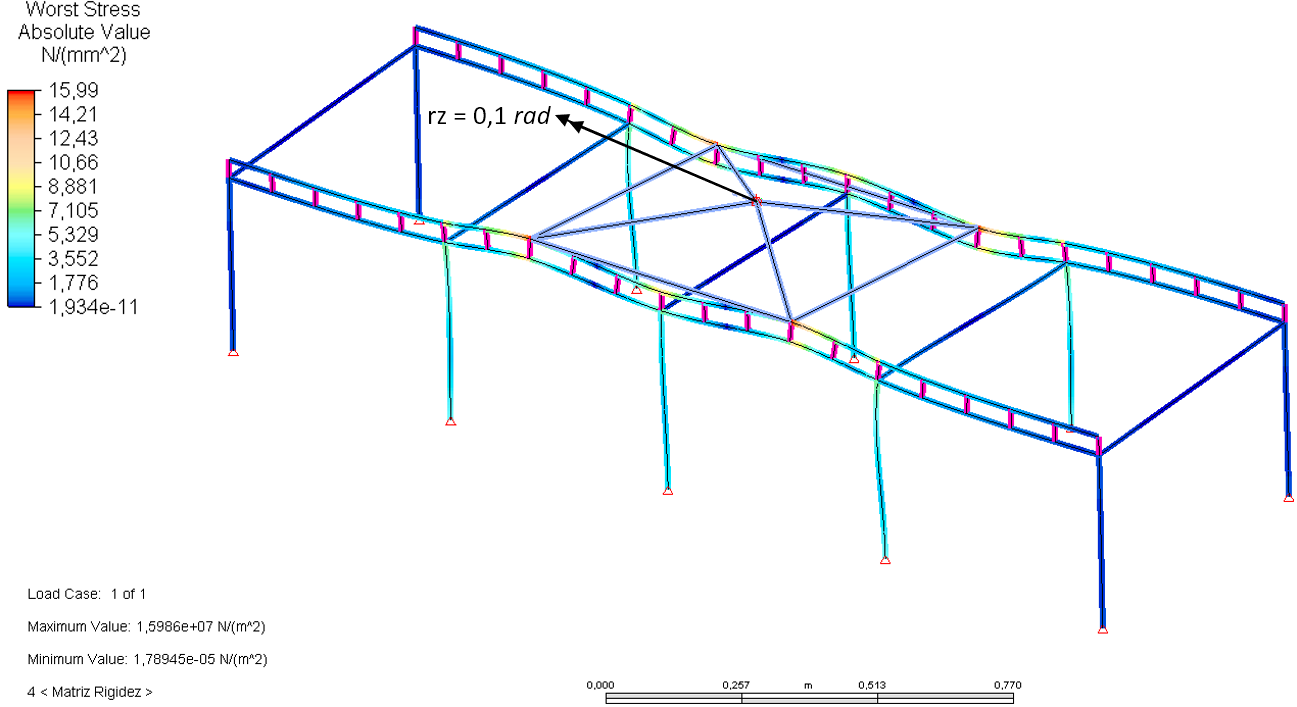
\includegraphics[width=\textwidth]{figs/res_FEA_tensoes}
        \caption{Resultado AEF das tensões máximas resultantes}
        \label{fig::res_FEA_tensoes}
    \end{subfigure}
    \quad %add desired spacing between images, e. g. ~, \quad, \qquad, \hfill
    % etc.
      %(or a blank line to force the subfigure onto a new line)
    \begin{subfigure}[b]{0.90\textwidth}
        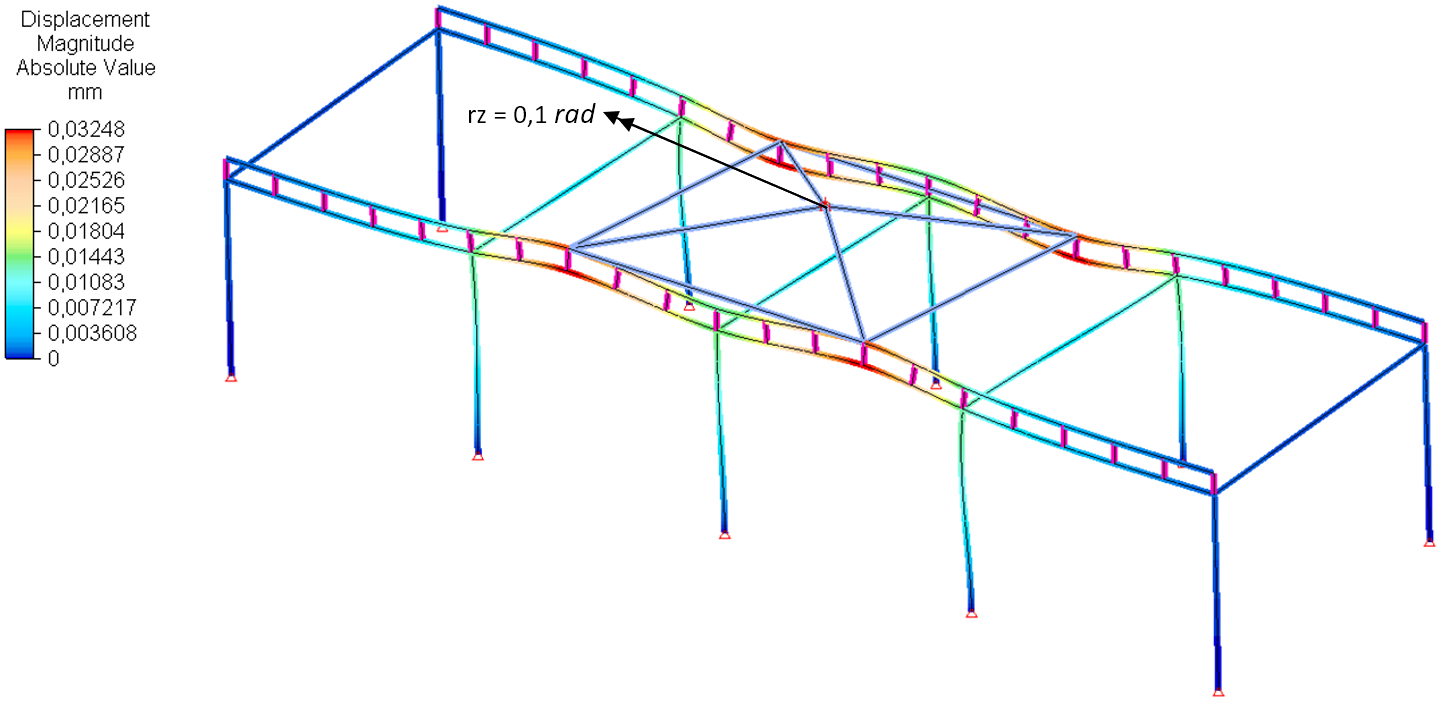
\includegraphics[width=\textwidth]{figs/res_FEA_desloc}
        \caption{Resultado AEF dos deslocamentos resultantes}
        \label{fig::res_FEA_desloc}
    \end{subfigure}
    \caption{Resultado da simulação AEF para o caso 6}
    \label{fig::res_FEA}
\end{figure}

O resultado das forças e momentos de reação no ponto de fixação do robô é
apresentado na Tabela~\ref{tab::res_FEA_forcas}. 

\begin{table}[h!]
\centering
\caption{Resultado das forças e momentos de reação para o caso 6}
\label{tab::res_FEA_forcas}
\begin{tabular}{@{}ccccccc@{}}
\toprule
\textbf{Caso} & \textbf{Fx [kN]} & \textbf{Fy [kN]} & \textbf{Fz [kN]} &
\textbf{Mx [kNm]} & \textbf{My [kNm]} & \textbf{Mz [kNm]} \\ \midrule \textbf{6}   
& -3,00E-9 & 2,50    & 1,67E-10    & 1,12E-9    & -7,16E-10   & -9,76   \\
\bottomrule
\end{tabular}
\end{table}

\subsubsection{Frequências Naturais}

O modelo AEF permite ainda obter as frequências naturais da base. O Autodesk
Simulation Mechanical efetua esta análise como uma simulação linear. São
analisados 2 casos: no primeiro, o peso e inércia do robô são adicionados ao
modelo e são aplicados no ponto virtual da base, no segundo caso sumprime-se a
inércia do robô. Isto permite verificar o comportamento da base para o caso de
operação e de testes do ensaio experimentais. A
Tabela~\ref{tab::freq_naturais_teste} apresenta o resultado das 10 primeiras
frequências naturais calculadas, em cada caso.

\begin{table}[h]
\centering
\caption{Frequências naturais pela AEF}
\label{tab::freq_naturais_teste}
\begin{tabular}{ccccccccccc}
\hline
\textbf{Modo}          & \textbf{}       & 1   & 2   & 3   & 4   & 5   & 6   & 7   & 8   & 9   \\ \hline
\textbf{Freq. Natural} & \textbf{c/robô} & 101 & 138 & 264 & 293 & 326 & 415 & 714 & 715 & 757 \\
\textbf{{[}Hz{]}}      & \textbf{s/robô} & 228 & 263 & 264 & 362 & 415 & 714 & 716 & 761 & 846 \\ \hline
\end{tabular}
\end{table}



\subsection{Matriz de Rigidez}

A base é simplificada como um sistema massa-mola-amortecedor de
6 gdl e rigidez $K$ introduzida no modelo MBS como uma matriz $6 \times 6$, que
relaciona os deslocamentos com o carregamento resultante da dinâmica do robô.

A matriz de rigidez possui portanto 36 termos, chamados de coeficientes de
influência. Cada termo na matriz está relacionado à direção da força e do
momento aplicado. Assim, o termo $k_{32}$ por exemplo refere-se a rigidez na
direção $y$, devido a uma força na direção $z$. A matriz de rigidez tem a
seguinte forma:
%
\begin{equation}
K = \begin{pmatrix} 
    k_{11} & \dots 	& k_{16} \\
    \vdots & \ddots & \\
    k_{61} &        & k_{66} 
    \end{pmatrix}
\end{equation}
%
Com o resultado das análises por AEF de cada caso, calcula-se os coeficientes de
influência da matriz de rigidez. Faz-se o
seguinte cálculo para normalizar o coeficiente de influência para valores
unitários de deslocamento:
%
\begin{align} \label{eq::kij}
	k_{ij} = \frac{F_j}{u_{i}} \qquad &  i,j = 1,\ldots,6
\end{align}
%
Onde $u_i$ representa o valor do deslocamento prescrito e $F_j$ o valor da força
ou momento de reação em cada caso de carregamento.
A matriz de rigidez é sempre positiva
definida~\cite{adhikari2004rayleigh}, ou seja, simétrica e com
seus autovalores positivos.
Isso faz com que não seja necessário calcular todos os 36 coeficientes de influências, mas apenas 21. 

Utilizando os resultados das simulações AEF e a equação~\ref{eq::kij}, a matriz
de rigidez para a base de testes é:
%
\begin{equation*}
	K =
\begin{pmatrix}
941537	&	0	&	0	&	0	&	0	&	0 \\
0	&	130543	&	0	&	0	&	0	&	-24981 \\
0	&	0	&	262149	&	0	&	5757	&	0 \\
0	&	0	&	0	&	57019	&	0	&	0 \\
0	&	0	&	5757	&	0	&	119561	&	0 \\
0	&	-24981	&	0	&	0	&	0	&	97595 \\
\end{pmatrix}
\end{equation*}
%
Os valores da matriz são expressos em $kN/m$ para os termos relacionados à
rigidez de translação e $kNm/rad$ para os termos relacionados à rigidez
torsional.
Os termos que aparecem zerados não são exatamente zero, mas valores muito
pequenos e, por simplificação, foram considerados nulos.


\subsection{Matriz de Amortecimento}

O amortecimento será modelado como proporcional, ou de Rayleigh, como
apresentado na seção~\ref{sec::amortecimento}. A matriz de amortecimento é
definida, pela equação~\ref{eq::amort_prop}, repetida a seguir:
%
\begin{equation*}
	C = \alpha M + \beta K
\end{equation*}
%
Logo, para definir totalmente a matriz de amortecimento da base, basta fornecer
os dois parâmetros, $\alpha$ e $\beta$.

Na seção~\ref{sec::amortecimento_revbib} apresentou-se um método para, a partir dos dados
experimentais de amortecimento modal, obter os parâmetros $\alpha$ e $\beta$ que
melhor se ajustam ao modelo. Na seção~\ref{sec::experimento} é
detalhado o procedimento para se obter os valores experimentais de amortecimento
e, a partir do resultado, calcular os os coeficientes de Rayleigh e obter a
matriz de amortecimento.



\subsection{Modelo teórico MBS -- Base}

O Sophia-Maple é utilizado para a construção do modelo cinemático e
cálculo das equações de movimento do sistema MBS da base, assim como foi
realizado o modelo do robô. Por isso, os comandos e sintaxe do Sophia,
apresentados na seção~\ref{sec::dkin}, não serão repetidos nesta seção, ciente
da equivalência do procedimento.

Para se chegar às equações de movimento, primeiramente, define-se os sistemas de
coordenadas e as coordenadas generalizadas do sistema.
As variáveis $q1, q2$ e $q3$ representam as 3 translações do ponto virtual de
fixação do manipulador, em $x,y$ e $z$, respectivamente, em relação ao sistema de
coordenadas inercial, SC-R. As 3 rotações são representadas pelas variáveis
$q4, q5$ e $q6$ e são descritos nos sistemas de coordenadas SC-R1, SC-R2,
SC-R3, respectivamente.
A coordenada $q4$ representa o ângulo de rotacão do sistema SC-R1
em relação ao sistema SC-R; $q5$ o ângulo entre SC-R2 e SC-R1; e $q6$ o ângulo
entre SC-R3 e SC-R2. A Figura~\ref{fig::schem_scbase} ilustra o sistema inercial
SC-R e o sistema SC-R3 acoplado ao corpo sobre a base.

\begin{figure}[h]
	\centering 
 	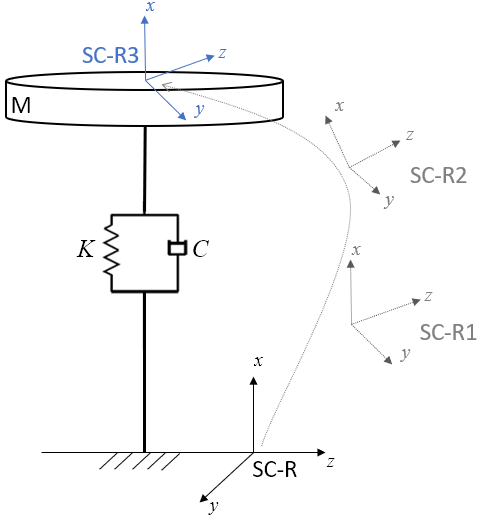
\includegraphics[width=0.40\textwidth]{figs/schem_scbase}
 	\caption{Desenho esquemático dos sistemas de referência da base e inercial}
 	\label{fig::schem_scbase}
\end{figure}

Neste modelo é considerado apenas um corpo, descrito em SC-R e localizado pelo
vetor $\mathbf{p}^M$, função de $q1,q2$ e $q3$.
%
\begin{equation}
	\mathbf{p}^M = [q1,~q2,~q3]^R
\end{equation}
%
Logo, se não há deslocamento da base ($q1=q2=q3=0$) então estará coincidente com
o ponto zero, do referencial inercial.

Seguindo o cálculo da cinemática, obtém-se os vetores velocidades e acelerações
angulares, exatamente como realizado na seção~\ref{sec::dkin}, mas desta vez
apenas para o corpo $M$.
Portanto, a equação~\ref{eq::velocM} calcula a velocidade do corpo, pela
derivada temporal do vetor posição em relação a SC-R. E a equação,
\ref{eq::velangM} calcula o vetor velocidade angular de $M$, no referencial SC-R
em relação ao referencial SC-R3, que considera as 3 rotações $q4, q5$ e $q6$ da
base.
%
\begin{gather} 
%eq1	
	^{R}\mathbf{v}^{M} = [u1,~u2,~u3]^R \label{eq::velocM} \\
%eq2
	\boldsymbol{\omega}^{M} = ^{R}\boldsymbol{\omega}^{R3} = [{\it s5}\,{\it
	u6}+{\it u4},-{\it c5}\,{\it s4}\,{\it u6}+{\it c4}\,{ \it u5},{\it c5}\,{\it c4}\,{\it u6}+{\it s4}\,{\it u5}]^{R}
\label{eq::velangM}
\end{gather}
%

Em seguida é composto o vetor das Velocidades Generalizadas e calculado o
Hiperplano Tangente.
%
\begin{gather}
	\mathbf{v}_{gen} = [ \mathbf{v}^{M},~ \boldsymbol{\omega}^{M}] \\
	\boldsymbol{\tau} = [\boldsymbol{\tau}_1,~ \boldsymbol{\tau}_2]
\end{gather}
%

O cálculo das equações dinâmicas se divide em definir o vetor das Forças
Externas generalizadas e o vetor das Forças de Inércia generalizadas, para, em
seguida, projetá-los no hiperplano tangente e obter as equações de movimento.

As forças externas são formadas pela força peso, do corpo $M$ e
pelas forças conservativas e não conservativas da base, provenientes da rigidez
e do amortecimento. Portanto:
%
\begin{equation}
	\mathbf{Peso}_M = m_M \cdot \mathbf{g}
\end{equation}
%
O termo $m_M$ representa o valor da massa suspensa pela base. O vetor
gravidade é descrito no referncial inercial SC-R.
%
\begin{equation}
	\mathbf{g} = [-9,81,~0,~0]^{R}
\end{equation}
%

% Neste tópico de apresentação do modelo desacoplado da base, o valor desta massa
% será a massa total do robô, $130~kg$.

As forças conservativas são calculadas pela matriz de rigidez da base. Esta
matriz, multiplicada pelo vetor das coordenadas generalizadas, fornece um
conjunto de 6 equações, que retornam a força elástica em função dos
deslocamentos do corpo.
%
\begin{equation}
%eq1
	\mathbf{Fk} = \mathbf{K} \cdot \mathbf{q}
\end{equation}
\begin{equation}
%eq2
	\mathbf{Fk} = \begin{pmatrix} 
    k_{11} & \dots 	& k_{16} \\
    \vdots & \ddots & \\
    k_{61} &        & k_{66} 
    \end{pmatrix} \cdot 
    \begin{pmatrix} 
    q1 \\ 
    \vdots \\ 
    q6 
    \end{pmatrix}
\end{equation}


Logo, a equação~\ref{eq::fki} calcula a força elástica $Fk$ na direção $i$
associada a cada coordenada generalizada $qi$:
%
\begin{equation} \label{eq::fki}
	Fk_i = \sum_{j=1}^{6} k_{ij} \cdot q_j
\end{equation}
%
Note-se que é utilizado o termo forças de forma generalizada para designar tanto
as forças lineares quanto momentos.

Equivalentemente, obtém-se as expressões para as forças não conservativas, mas
desta vez, multiplica-se a matriz de amortecimento $C$ pelo vetor $u$ das
velocidades. Logo:
%
\begin{equation} \label{eq::fci}
	Fc_i = \sum_{j=1}^{6} c_{i,j} \cdot u_j
\end{equation}
%
Onde o termo $c_{ij}$ refere-se aos coeficientes da matriz de amortecimento.

O equilíbrio das forças que agem sobre o corpo suspenso pela base são:
%
\begin{equation} \label{eq::fexm}
	\mathbf{Fex}_M = \mathbf{Peso}_M - \mathbf{Fk} - \mathbf{Fc}
\end{equation}
%
As forças externas genearlizadas são a projeção do vetor das forças externas da
equação~\ref{eq::fexm} no hiperplano tangente $\tau$.
%
\begin{equation}
	\mathbf{FEX}g = \mathbf{Fex}_M \cdot \boldsymbol{\tau}
\end{equation}
%

As forças de inércia são calculadas pelas equações~\ref{eq::finG} e
\ref{eq::finH}, para o corpo $M$. Aplicando ao modelo da base, obtém-se as
forças de inércia generalizadas, pela projeção do vetor forças de inércia no
hiperplano tangente $\tau$.
%
\begin{gather}
	\mathbf{Fin}_M = [\dot{\mathbf{G}}_{M},~ \dot{\mathbf{H}}_{M}] \\
	\mathbf{FIN}g = \mathbf{Fin}_M \cdot \boldsymbol{\tau}
\end{gather}
%
Finalmente, a equação de movimento do corpo $M$ é obtida pelo equilíbrio das
forças externas e de inércia generalizadas. Portanto, tem-se 6 equações de
movimento, associadas aos 6 gdl do sistema:
%
\begin{equation}
	\mathbf{FEX}g - \mathbf{FIN}g = \mathbf{0}
\end{equation}
%
O sistema \textit{kinematic differential equation} (kde) fornece mais 6
equações, relacionando $q$ e $u$. As condições iniciais $q1(0),\ldots,q6(0)$ e
$u1(0),\ldots,u6(0)$ completam o problema.

Assim como no MBS do robô, o problema consiste em solucionar um sistema de
equações diferenciais ordinárias, não-lineares, cujas incógnitas são as
coordenadas generalzadas $q1(t),\ldots,q6(t)$ e as velocidades
$u1(t),\ldots,u6(t)$. 

Para demonstrar o modelo, considere-se os seguintes parâmetros de rigidez,
amortecimento e condição incial do sistema:
%
\begin{itemize}
  \item{\textbf{Rigidez:} igual a da base de testes}
  \item{\textbf{Amortecimento:} $\alpha = 0;~ \beta = 10^{-4}$}
  \item{\textbf{Condição inicial:} $q1(0) = q2(0) = q3(0) =1~mm$, $q4(0) =
  0,001~rad$, $q5(0) = q6(0) = 0$}
\end{itemize}
%


\subsubsection{Resultados do exemplo}

A Figura~\ref{fig::res_qbase_exemplo} apresenta o resultado dos deslocamentos da
base, dada a condição incial fora da sua configuração de equilíbrio.

\begin{figure}[h]
    \centering
    \begin{subfigure}[b]{0.80\textwidth}
        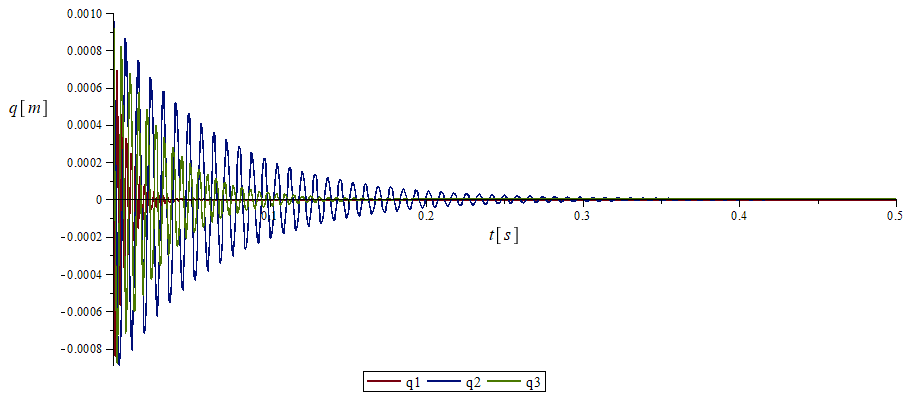
\includegraphics[width=\textwidth]{figs/q123_base_exemplo}
        \caption{Resultado MBS da base: translações q1, q2, q3}
        \label{fig::q123_base_exemplo}
    \end{subfigure}
    \quad %add desired spacing between images, e. g. ~, \quad, \qquad, \hfill
    % etc.
      %(or a blank line to force the subfigure onto a new line)
    \begin{subfigure}[b]{0.80\textwidth}
        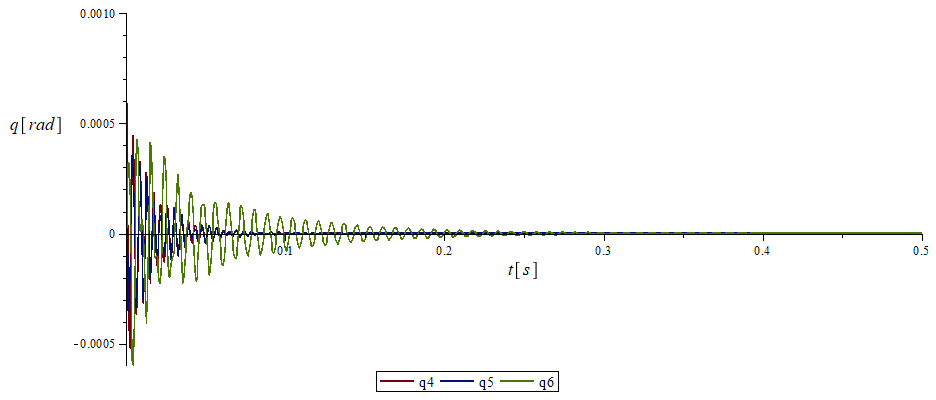
\includegraphics[width=\textwidth]{figs/q456_base_exemplo}
        \caption{Resultado MBS da base: rotações q4, q5, q6}
        \label{fig::q456_base_exemplo}
    \end{subfigure}
    \caption{Resultados dos primeiros 500~ms do deslocamento da base}
    \label{fig::res_qbase_exemplo}
\end{figure}

Note-se que, antes do tempo final da simulação, o sistema parece estar em
equilíbrio. O resultado de cada coordenada generalizada em $t=0,5~s$ é:
%
\begin{align*}
	q1(0,5) &= -0,20839\cdot 10^{-5}~m \\
	q2(0,5) &= 4,8952\cdot 10^{-8}~m \\
	q3(0,5) &= 8,4009 \cdot 10^{-12}~m \\
	q4(0,5) &= -1,6031\cdot 10^{-10}~rad \\
	q5(0,5)	&= -1,6260\cdot 10^{-11}~rad \\
	q6(0,5) &= 1,7857\cdot 10^{-8}~rad
\end{align*}
%
Verifica-se por este resultado que, no equilíbrio, os deslocamentos são
desprezíveis para o robô, tal que os valores máximos são da ordem de
$10^{-2}~mm$ em $q1$ e $10^{-11}~rad$ em $q5$.








% -.~.-.~.-.~.-.~.-.~.-.~.-.~.-.~.-.~.-.~.-.~.-
\section{Ensaio Experimental} \label{sec::experimento}

Os parâmetros modais da base, associados aos modos e frequências naturais são
obtidos por meio de análise modal por ensaio de vibrações.
A estrutura de testes (Figura~\ref{fig::estrut_modelo_fisico}) é instrumentada
com acelerômetros a fim de se obter a dinâmica da base. Para o modelo
experimental foram selecionados 6 graus de liberdade para medição: as 3
translações e 3 rotações ortogonais do sistema de coordenadas cartesiano. Para
isso, foi idealizado um ponto para origem do sistema de coordenadas da base, que
é coincidente com o ponto teórico de fixação do robô. Logo, os 6 graus de
liberdade estão associados às translações e rotações em relação ao sistema de
coordenadas fixo neste ponto.
Um martelo instrumentado é utilizado para excitar a base e obter as Funções de
Resposta em Frequência (FRF's) de cada grau de liberdade.
Estes dados são utilizados para estimar os parâmetros modais:
modos de vibração, frequências naturais e amortecimentos, pelo procedimento
chamado Ajuste de Curva (\textit{Cuve Fitting}).
Os resultados experimentais são então utilizados para calcular os parâmetros
$\alpha$ e $\beta$ da matriz de amortecimento proporcional.


\subsection{Bancada experimental e instrumentação}

A base de testes é utilizada para os propósitos do ensaio e instrumentada com
acelerômetros. Para ter consistência entre os modelos teórico e experimental,
deseja-se obter as acelerações de um ponto virtual, localizado no centro da
placa de fixação do robô. Este ponto representa a conexão teórica entre a base e
o manipulador, que restringe qualquer translação ou rotação relativa entre eles.
Definindo-se um referencial local neste ponto, qualquer deslocamento e rotação
é transferido diretamente para o manipulador. Logo, este
ponto está para o modelo experimental assim como $\mathbf{p}^M$ está para o
modelo teórico da base. Da mesma forma, o referencial local da placa é
equivalente ao referencial SC-R3 do modelo teórico.

\begin{figure}[h]
	\centering 
 	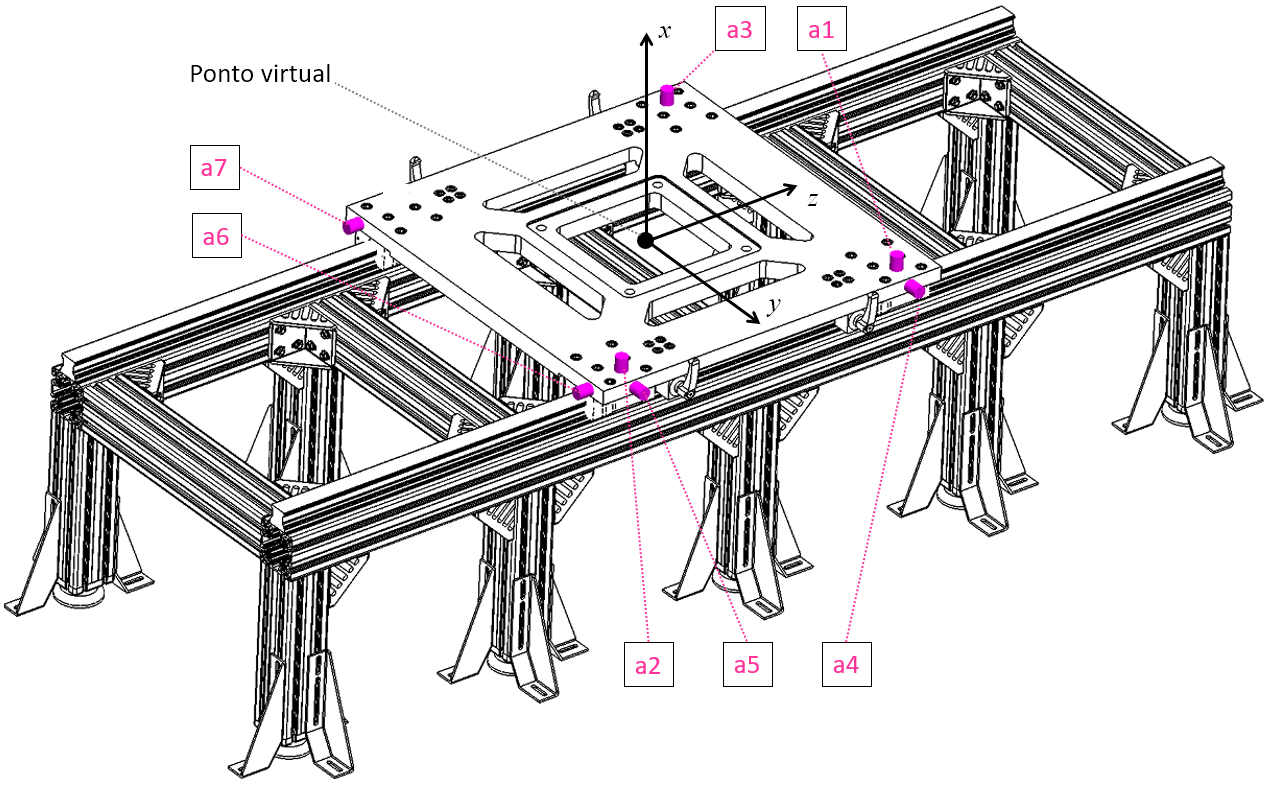
\includegraphics[width=0.95\textwidth]{figs/acelerometos-base}
 	\caption{Dsitribuição dos acelerômetros na base}
 	\label{fig::acelerometos-base}
\end{figure}

\subsubsection{Acelerômetros}

São utilizados no total 7 acelerômetros uni-axiais piezoelétricos, fixados à
placa por bases magnéticas. A Figura~\ref{fig::acelerometos-base} apresenta a
distribuição dos acelerômetros na estrutura, onde são representados pelos
pequenos cilindros indicados, cuja direção de medição é a mesma do seu eixo, e o
sentido positivo sempre para fora da placa.

Assim como foi assumido no modelo para AEF da base, a placa de fixação do robô é
muito rígida em relação à estrutura de perfis de alumínio. Ou seja, as
deformações desta peça são relativamente despezíveis e portanto a distância
entre quaisquer dois pontos sobre a placa permanecerá fixa no referencial local.
Isto permite a distribuição dos acelerômetros em qualquer ponto da placa.

Isto implica, que pode-se calcular a aceleração, em cada uma das 6 direções do
ponto virtual, a partir de relações aritméticas simples entre os sensores $a1$ a
$a7$. As acelerações lineares são indicadas pela variável $a$ e as
rotacionais por $\alpha$ seguidas de subíndice indicando sua orientação. Logo:
%
\begin{align}
	a_x &= \frac{a2+a3}{2} \label{eq::acel_ax}\\
	a_y &= \frac{a4+a5}{2} \\
	a_z &= - \frac{a6+a7}{2} \\
	\alpha_x &= \frac{a5-a4}{r1} \\
	\alpha_y &= \frac{a2-a1}{r1} \\
	\alpha_z &= \frac{a1-a3}{r2} \label{eq::acel_alphaz}
\end{align}
%
Onde $r1$ é a distância entre os acelerômetros $a1$ e $a2$, na direção $z$; e
$r2$ a distância entre os acelerômetros $a6$ e $a7$, na direção $y$.

Note-se que as acelerações lineares são calculadas pela média entre dois
acelerômetros na mesma direção.
Já as acelerações angulares, pela diferença entre os dois acelerômetros na mesma
direção, dividida pela distância, $r1$ ou $r2$ entre eles. Considere-se agora
que cada equação crie um sensor virtual, localizado no centro entre o par
calculado. Se a placa é rígida, pode-se considerar então que tais acelerações
são as mesmas correspondentes às do ponto central
da placa.

Tem-se portanto um vetor das acelerações generalizadas medidas no referencial
local da placa, em que cada termo representa uma direção dos 6 gdl da base.
%
\begin{equation}
	\mathbf{a} = \left[ a_x, a_y, a_z, \alpha_x, \alpha_y, \alpha_z \right]
\end{equation}
%

\subsubsection{Martelo Instrumentado}

A excitação da estrutura é feita com um martelo instrumentado com sensor de
força piezoelétrico, da fabricante PCB. Pelo tamanho e peso da estrutura a ser
testada, é recomendável um impacto com energia suficiente para excitar toda a
estrutura, a fim de obter os modos de vibração em uma faixa suficientemente
larga de frequência. A energia do impacto pode ser calculada por:
%
\begin{equation}
	E = m \cdot v
\end{equation}
%
Infere-se que, para ter uma energia mais alta, ou aumenta-se a velocidade do
impacto, ou a massa do martelo. Como os modelos de martelo com massa baixa
($<1~kg$) não seriam capazes de excitar a estrutura adequadamente, optou-se por
um martelo de massa elevada. O modelo PCB-086D50 foi escolhido para o ensaio.
Este martelo possui massa de $5,5~kg$ e faixa de medição de $\pm 25~kN$.

A faixa de frequência excitada é função do material da ponta do martelo.
A Figura~\ref{fig::carta_badwidth} apresenta a força do impacto no espectro das
frequências, obtida pela \textit{Fast Fourier Transform} (FFT) a partir do sinal
no tempo.
Percebe-se que para uma mesma força de pico do impacto, uma ponta mais dura
resulta em uma faixa mais larga de frequência.

\begin{figure}[h!]
	\centering 
 	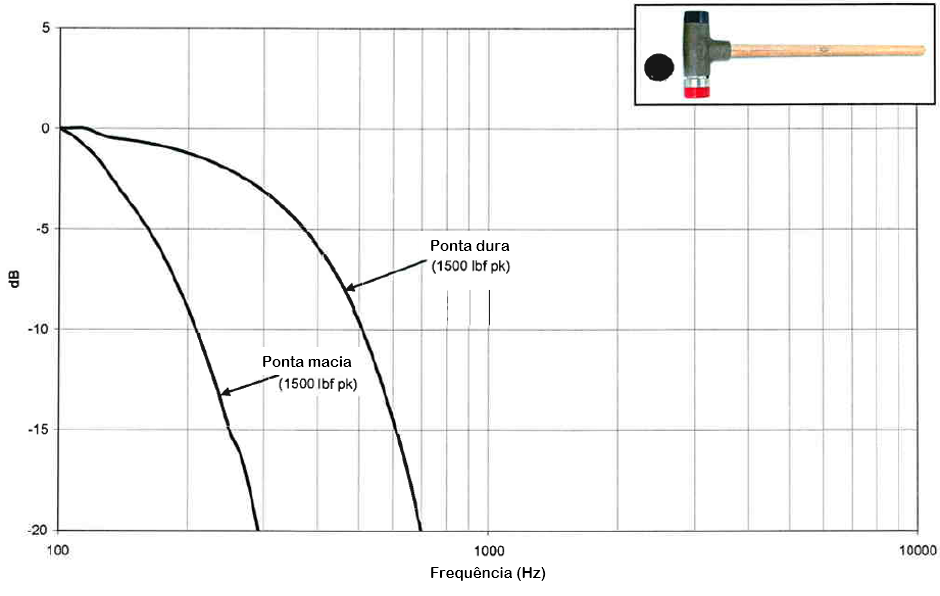
\includegraphics[width=0.82\textwidth]{figs/carta_badwidth}
 	\caption[Espectro de frequência do impacto do martelo PCB-086D50]{Espectro de
 	frequência do impacto do martelo PCB-086D50. \\	Fonte: adaptado de~\cite{manualpcb} }
 	\label{fig::carta_badwidth}
\end{figure}


\subsubsection{Placas de aquisição, chassi e programas}

Para aquisição dos dados experimentais são utilizadas duas placas NI-9234, da
fabricante National Instruments. Cada placa possui 4 canais. Uma placa recebe 4
acelerômetros e a outra 3, mais o martelo instrumentado.

Um chassi portátitil modelo NI cDAQ-9178 com capacidade de até 8 placas
de aquisição controla a temporização, sincronização e transferência dos dados
para o computador, via USB. 

O programa SignalExpress fornece uma interface para registro, leitura gráfica,
análise e pós processamento dos dados adquiridos. É utilizado para realizar
a média das aquisições, cálculo das acelerações em cada direção, FFT do impacto
do martelo e a Função Resposta em Frequência (FRF) das acelerações.

Obtidas as FRF's das acelerações em cada direção, os resultados de
magnitude e fase das FRF's são importados no programa ME'Scope VES, que oferece
ferramentas prontas para análise modal e obtenção dos modos, frequências
naturais e amortecimentos.

A Figura~\ref{fig::foto_bancada} apresenta uma fotografia da bancada
experimental, montada no Laboratório de Acústica e Vibrações (LAVI/COPPE-UFRJ) e
a Figura~\ref{fig::diagrama_bancada} um diagrama esquemático, indicando os
sensores, a base e os módulos de aquisição, assim como as conexões entre eles.

\begin{figure}[h]
	\centering 
 	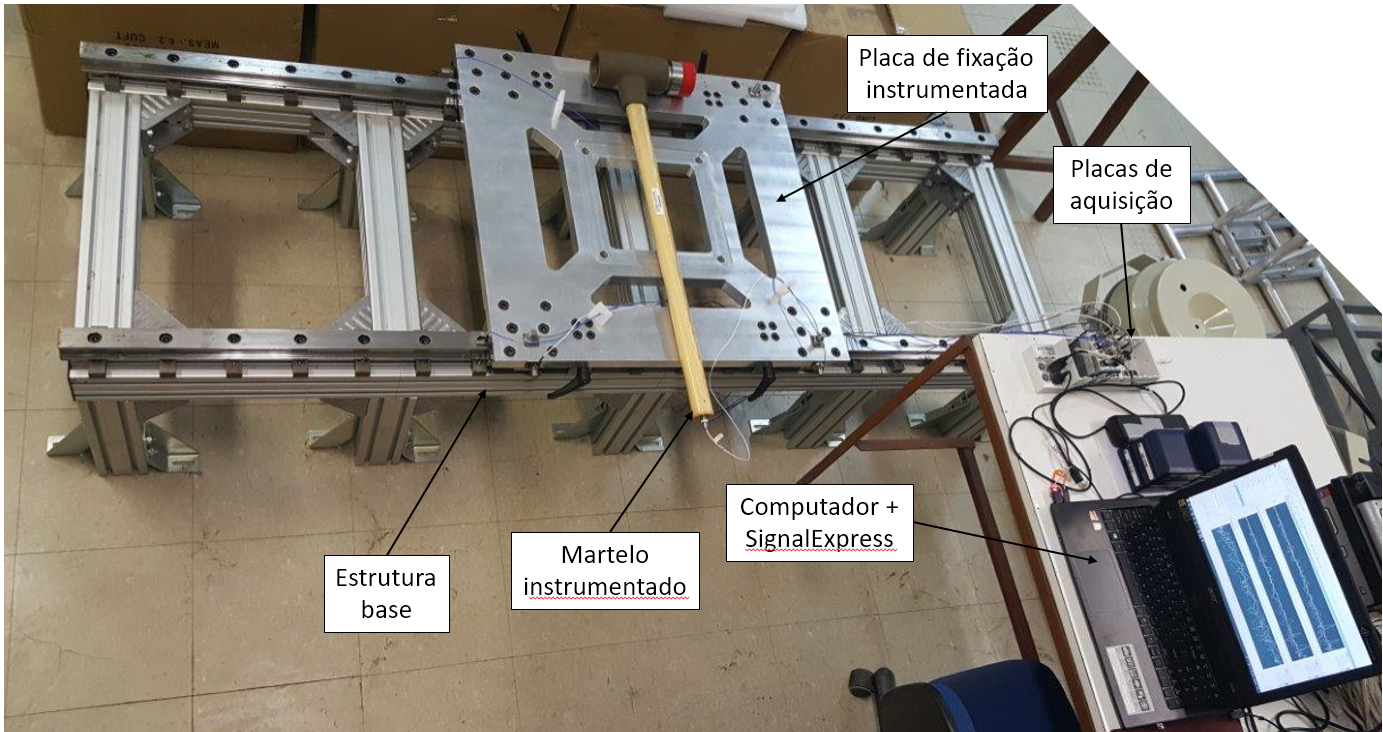
\includegraphics[width=0.95\textwidth]{figs/foto_bancada}
 	\caption{Aparato da bancada experimental no laboratório}
 	\label{fig::foto_bancada}
\end{figure}

\begin{figure}[h]
	\centering 
 	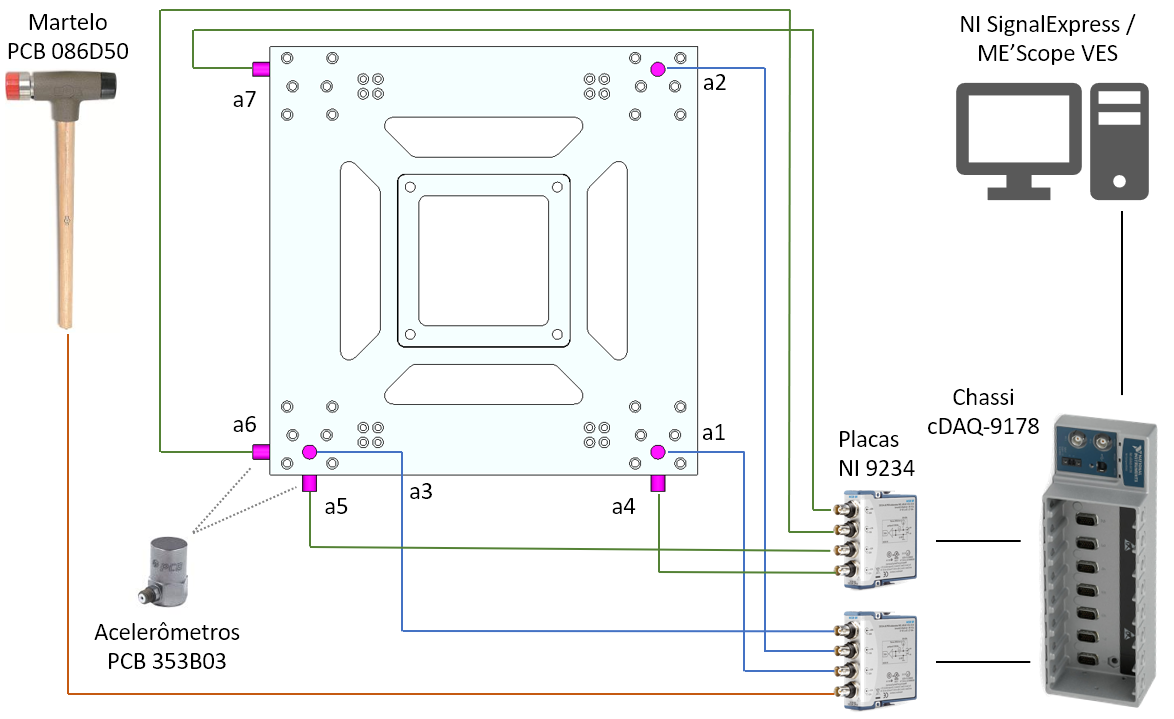
\includegraphics[width=0.95\textwidth]{figs/diagrama_bancada}
 	\caption{Diagrama da bancada experimental}
 	\label{fig::diagrama_bancada}
\end{figure}


\subsection{Aquisição e tratamento dos dados}

Os dados coletados pelos acelerômetros e o martelo instrumentado são enviados
através das placas e chassi de aquisição para tratamento, em tempo real no
SignalExpress. O pós-processamento no programa calcula as FRF's de cada grau de
liberdade e os resultados são exportados para o ME'Scope para realizar análise
modal e estimativa dos parâmetros modais. Segue o detalhamento de cada uma
destas etapas.

\subsubsection{Aquisição no SignalExpress}

Antes de serem adquiridos, deve-se primeiro preparar o ambiente no
programa SignalExpress. Nele é mapeado o canal que receberá os dados
de cada sensor, fornecidos os tipos de sensores e os valores de sensibilidade,
faixas de trabalho, taxa de aquisição e número de amostras.

Para evitar os fenômenos de \textit{aliasing}, a taxa de aquisição foi definida
em $20~kHz$, longe o suficiente da frequência de
ressonância esperada da base, e para evitar o vazamento espectral (ou
\textit{leakage}), o número de amostras como o dobro da taxa, neste caso, $40$
mil. Isto garante uma janela de tempo de cada amostragem de 2 segundos. Como o
sinal é quase totalmente amortecido neste intervalo de tempo, não há necessidade
de utilizar uma função de janelamento (ou \textit{window}) neste sinal.
É utilizada a função \textit{Averaging} para calcular a média das amostragens,
pelo método RMS (\textit{Root Mean Square}).
Serão coletadas 5 amostragens por direção de estímulo, para processamento e
cálculo dos dados.

Em seguida, são definidas as acelerações do ponto central da base, que são
calculadas pelas equações~\ref{eq::acel_ax} a \ref{eq::acel_alphaz}. No
SignalExpress é utilizada a função de pós-processamento \textit{Formula}, que
permite realizar operações algébricas entre até 4 sinais. Logo, são definidas 6
funções que calculam as acelerações do ponto virtual central da base.

Por fim, é utilizada a função \textit{Frequency Response} do pacote NI Sound and
Vibration Assistant do SignalExpress. Esta função recebe  os sinais do
martelo e as acelerações em uma direção, e calcula as FRF's
entre as acelerações (saída) e a força de impacto (entrada).

\subsubsection{Função de Transferência}

Seja a Função de Transferência definida por uma matriz $H_{n \times n}$, formada
pelos termos $h_{ij}$. Cada termo representa uma FRF da aceleração de cada
direção $i$ como resposta do impulso do martelo na direção $j$. Logo, para este
modelo de base, $n$ é igual ao número de graus de liberdade, 6. Portanto 36
termos definem a Função de Transferência deste modelo. Como a matriz é
simétrica, podem ser deteminados apenas 21 dos 36 termos.
%
\begin{equation}
H =
\begin{pmatrix}
    h_{11} & h_{12} & h_{13} & h_{14} & h_{15} & h_{16} \\
		   & h_{22} & h_{23} & h_{24} & h_{25} & h_{26} \\
		   & 		& h_{33} & h_{34} & h_{35} & h_{36} \\
		   & 		&  		 & h_{44} & h_{45} & h_{46} \\
		   & 		&  		 &  	  & h_{55} & h_{56} \\
      \multicolumn{2}{c}{\text{sim.}} & & &    & h_{66} 
\end{pmatrix}
\end{equation}
%

Note-se que para calcular os termos devido a rotação da base $h_{i4}$ a
$h_{i6}$, então seria necessário excitar um momento em cada direção angular
($r_x,r_y,r_z$). Entretanto, é inviável excitar, com o martelo, um
momento puro na base. Logo, estes termos não podem ser calculados diretamente.
Em compensação, o ensaio conta com aquisição simultânea de 6 sinais de saída
(acelerações) para cada sinal de entrada (impacto) e portanto classifica-se como
SIMO (\textit{Single Input Multiple Outputs}). A vantagem deste tipo de ensaio é
que para o caso em que o número de sinais é igual ao número de graus de
liberdade, obtem-se exatamente uma coluna inteira da matriz de Transferência. De
uma linha ou uma coluna completa, fornecendo informação suficiente para se
determinar os parâmetros modais.

\subsubsection{Resultados da aquisição}

A aquisição dos dados experimentais é feita realizando a média de 5 impactos na
mesma direção. A direção do impacto em $y$ foi escolhida por praticidade, já
que é possível acertar a estrutura muito próximo da direção do centro de massa e
portanto fornecer um estímulo em apenas uma direção.

Selecionou-se os dados tomados e processados em uma iteração da média
dos 5 impactos para representarem os resultados da aquisição. Na
Figura~\ref{fig::aceleracoes} apresenta-se as acelerações em cada grau de
liberdade medido da base e sobrepõe-se também o gráfico do impacto realizado
pelo martelo instrumentado.

\begin{figure}[h]
	\centering 
 	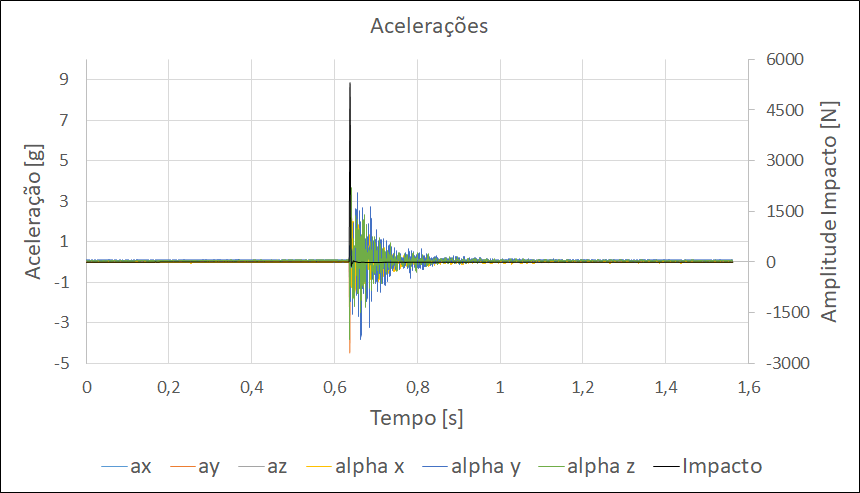
\includegraphics[width=0.95\textwidth]{figs/aceleracoes}
 	\caption{Dados experimentais das acelerações e magnitude do impacto vs. tempo
 	}
 	\label{fig::aceleracoes}
\end{figure}

A Figura~\ref{fig::martelo_spectrum} apresenta o resultado da transformação FFT
do impacto do martelo, fornecendo o espectro de frequência estimulado. Este
gráfico fornece um parâmetro para avaliar a faixa de frequência útil da medição.
Nota-se que de acordo com o resultado, a faixa útil do impacto é aproximadamente
de $0$ a $500~Hz$.

\begin{figure}[h!]
	\centering 
 	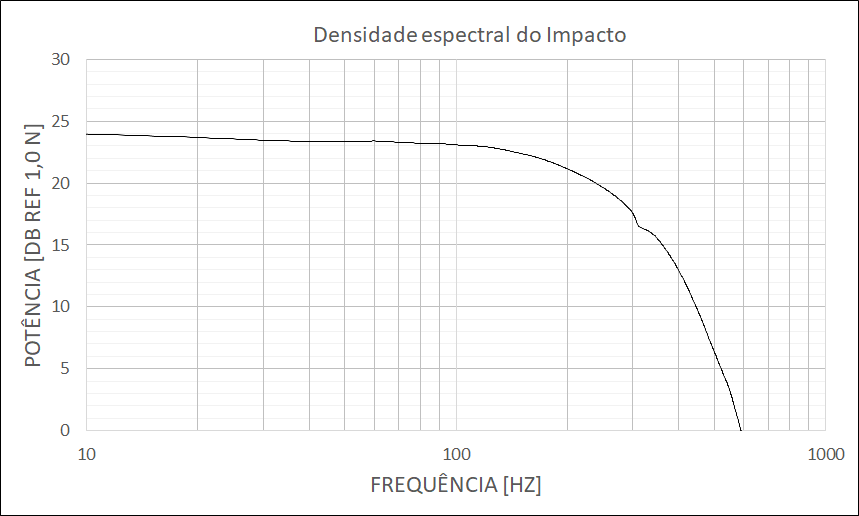
\includegraphics[width=0.95\textwidth]{figs/martelo_spectrum}
 	\caption{FFT do impacto do martelo}
 	\label{fig::martelo_spectrum}
\end{figure}

Por fim, o SignalExpress fornece a Função de Resposta em Frequência (FRF) de
cada grau de liberdade medido. O resultado da magnitude da FRF de cada gdl é
apresentado na Figura~\ref{fig::frfs} assim como sobrepõe o resultado da
Coerência do na direção $y$.

\begin{figure}[h]
	\centering 
 	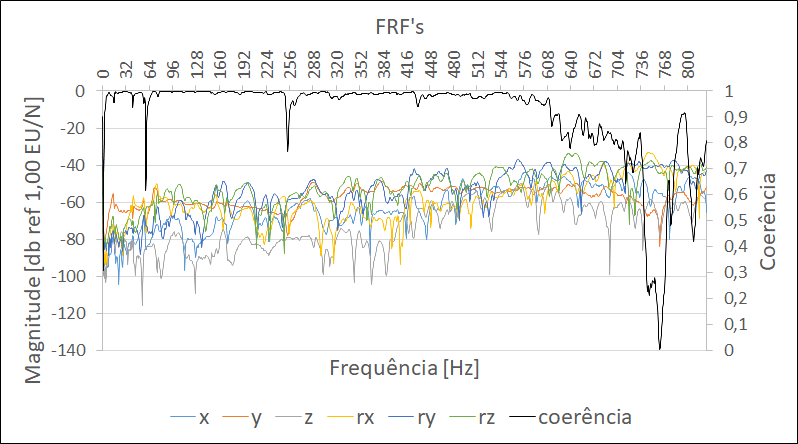
\includegraphics[width=0.95\textwidth]{figs/frfs}
 	\caption{Magnitude das FRF's para o impacto na direção $y$}
 	\label{fig::frfs}
\end{figure}

Verifica-se pelo espectro da coerência que a faixa de $0$ a $500~Hz$
continua uma boa estimativa quanto a qualidade do resultado, e portanto os dados
experimentais são adequados nesta faixa.





% Para verificar os resultados no SignalExpress, são reservadas áreas para
% plotagem dos seguintes gráficos:
% %
% \begin{itemize}
%   \item Acelerações $a_x, a_y, a_z, \alpha_x, \alpha_y, \alpha_y$ vs.
%   tempo;
%   \item Força do martelo vs. tempo;
%   \item FFT da força do martelo;
%   \item FRF's: $a_x, a_y, a_z, \alpha_x, \alpha_y, \alpha_y$ para $F_x, F_y,
%   F_z$: \\ Tal que em cada FRF fornece: Magnitude; Fase; parte Real; parte
%   Imaginária; e Coerência.
% \end{itemize}
% %
% Como são muitos, ao todo 27 gráficos, serão apresentados apenas os
% resultados para o ensaio de impacto na direção $y$ da base.

%\missingfigure{Resultado acelerações vs. tempo}

%\missingfigure{Resultado Força do martelo vs. tempo}

%\missingfigure{FFT da força do martelo}

%\missingfigure{FRF: Magnitude}

% \missingfigure{FRF: Fase}

% \missingfigure{FRF: Real}

% \missingfigure{FRF: Imaginário}

% \missingfigure{FRF: Coerência}


% A análise modal é realizada no programa ME'Scope. Para isso, os resultados devem
% ser exportados em arquivo ASCII na forma numérica, tal que a amostragem de dados
% estjeda disposta em colunas, na seguinte ordem:
% %
% \begin{equation*}
% \begin{matrix}
% Frequencia & Magnitude~\#1  & Fase~\#1  & \ldots & Magnitude~\#6 & Fase~\#6 \\ 
%  \vdots & \vdots & \vdots &  & \vdots & \vdots
% \end{matrix}
% \end{equation*}
% %
% As colunas de Magnitude e Fase correspondem aos
% resultados das 6 FRF's relativas aos 6 graus de liberdade coletados.

\subsubsection{Análise modal no ME'Scope}

O programa ME'SCope é utilizado para identificar os parâmetros modais a partir
das FRF's importadas. A interface de importação do programa ajuda a identificar
os dados e relacionar às direções de medição e excitação correspondentes.

A opção \textit{Modal Analysis} no ME'Scope é utilizada para identificar as
frequências de ressonância do sistema e estimar os parâmetros modais pela função
de ajuste de curva (\textit{curve fitting}). A primeira etapa é identificar a
faixa de frequência que se deseja analisar. Conforme foi identificado, será
analisada a faixa de $0$ a $500~Hz$. Em seguida, identifica-se os modos ou picos
nesta faixa. Ainda há opção da contagem automática, se fornecido um valor
mínimo de mangnitude para caracterizar o modo.

%\missingfigure{Inlcluir imagem da contagem de picos}

Com isso o programa realiza uma estimativa dos coeficientes de um polinômio do
modelo FRF analítico, pelo ajuste de curva ao modelo experimental.
% , apresentado
% na Figura~\ref{fig::curve_fitting}. 
% 
% \begin{figure}[h]
% 	\centering 
%  	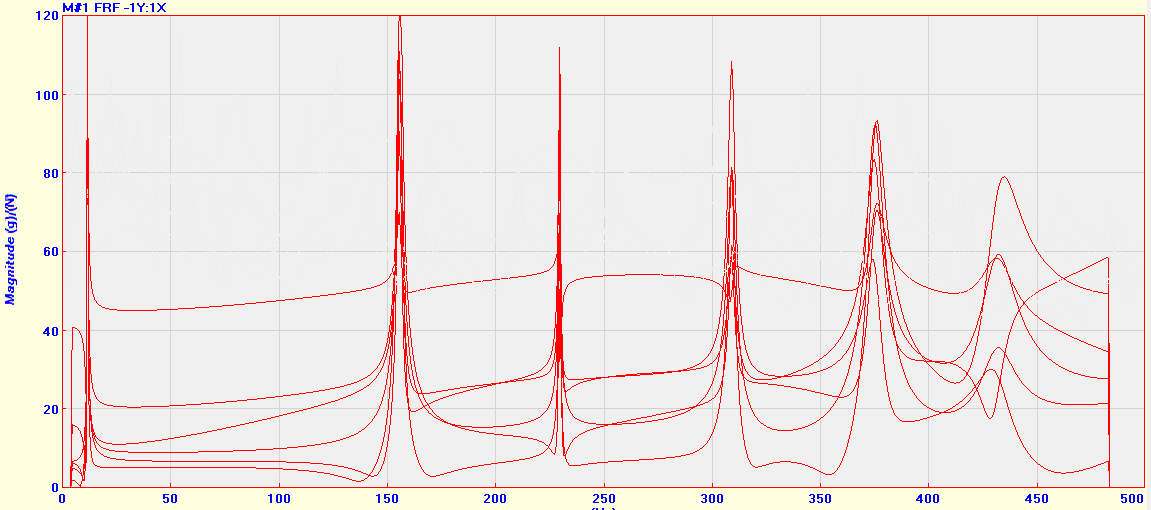
\includegraphics[width=0.95\textwidth]{figs/curve_fitting}
%  	\caption{Resultado do ajuste de curva das FRF's pela análise modal}
%  	\label{fig::curve_fitting}
% \end{figure}
Os coeficientes são então processados para obter os parâmetros modais. Os
resultados da análise modal encontram-se na
Tabela~\ref{tab::resultado_modal}.
%
\begin{table}[h]
\centering
\caption{Resultado do amortecimento modal}
\label{tab::resultado_modal}
\begin{tabular}{@{}cccc@{}}
\toprule
Modo & Frequência & Amortecimento {[}Hz{]} & Amortecimento {[}\%{]} \\ \hline
1    & 11,6       & 0,11                   & 0,947                  \\
2    & 156        & 1,06                   & 0,679                  \\
3    & 230        & 0,35                   & 0,151                  \\
4    & 309        & 1,61                   & 0,519                  \\
5    & 375        & 3,94                   & 1,050                  \\
6    & 432        & 8,45                   & 1,960                  \\ \hline
\end{tabular}
\end{table}
%

% O programa também permite construir o modelo 3D representando a estrutura com
% uma ferramenta de modelagem interativa. Pontos da malha que
% representa o modelo 3D são associados aos dados experimentais. Então é
% possível visualizar como a estrutura se comporta dinamicamente e, de forma
% interativa, visualizar uma animação dos modos de vibração. A
% Figura~\ref{fig::animacao_base} apresenta o modelo 3D da animação oscilando no
% primeiro modo de vibração.
% 
% \begin{figure}[h]
% 	\centering 
%  	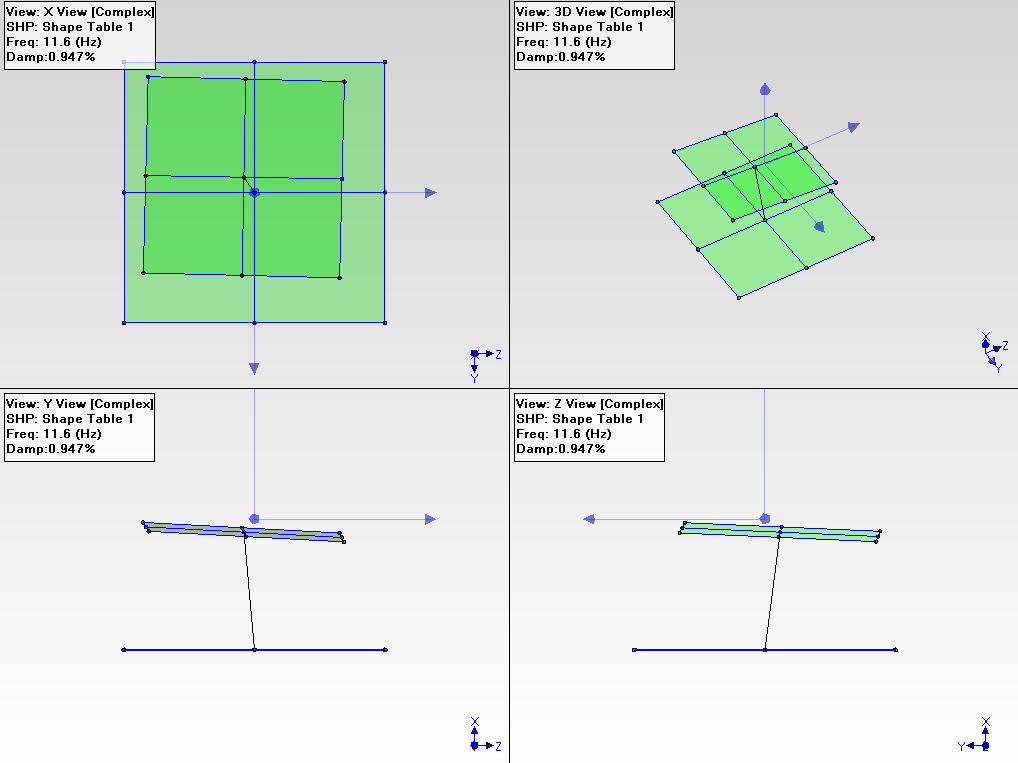
\includegraphics[width=0.95\textwidth]{figs/animacao_base}
%  	\caption{Animação do primeiro modo de vibração}
%  	\label{fig::animacao_base}
% \end{figure}


\subsection{Cálculo da Matriz de Amortecimento}

A matriz de amortecimento tem dimensão $6 \times 6$, que corresponde aos 6 graus
de liberdade (3 translações e 3 rotações) associados às coordenadas
generalizadas do modelo teórico. Para facilitar seu uso e generalização é
utilizado o modelo de amortecimento proporcional, em que assume-se
que o amortecimento depende apenas de dois parâmetros, $\alpha$
e $\beta$, proporcionais às matrizes de inércia e rigidez respectivamente, de
acordo com a expressão:
%
\begin{equation*}
	C = \alpha  M + \beta  K
\end{equation*}
%

Como demonstrado na seção~\ref{sec::amortecimento}, os parâmetros $\alpha$
e $\beta$ se baseiam no resultado do amortecimento modal ao longo de uma
faixa de frequência de interesse. Aplicando-se a equação~\ref{eq::brian} aos
resultados experimentais da Tabela~\ref{tab::resultado_modal}, tem-se:
%
\begin{equation} \label{eq::resmatrix_alpha_beta}
\begin{bmatrix}
	\alpha \\
	\beta
\end{bmatrix}
= 2
\begin{pmatrix}
	6 & 500087 \\ 
	500087 & 67111 \times 10^9
\end{pmatrix}^{-1}
\begin{bmatrix}
	17.407 \\ 
	2.32915 \times 10^6
\end{bmatrix}
\end{equation}

O resultado da equação~\ref{eq::resmatrix_alpha_beta} fornece:
%
\begin{align}
	\alpha &= 4,489 \times 10^-2 \\
	\beta &= 6,907 \times 10^{-5}
\end{align}
%

% E finalmente, a matriz de amortecimento resultante, obtida experimentalmente é:
% %
% \begin{equation}
% 	C = 4,489 \times 10^-2 ~M + 6,907 \times 10^{-5}~K
% \end{equation}
% %



% -.~.-.~.-.~.-.~.-.~.-.~.-.~.-.~.-.~.-.~.-.~.-
\section{Modelo acoplado robô e base} \label{sec::acoplado}

Demonstrou-se nas seções~\ref{sec::robo} e \ref{sec::base} como forma
construídos modelos dinâmicos do robô e da base em separado. Esta seção consiste
em unir os dois sistemas MBS em um modelo acoplado.
Isto é feito considerando que o sistema de coordenadas SC-Z, inercial no modelo
do robô, agora coincide com o sistema de coordenadas final do modelo da base,
SC-R3.

Note-se que no modelo da base, era considerado um único corpo, fixado no
``topo'' da cadeia cinemática de 6 graus de liberdade da base.
Agora, este corpo é representado pelo pedestal do robô, corpo Z, seguido dos 5
elos consecutivamente conectados, tornando-o um MBS de 11 graus de liberdade. A
Figura~\ref{fig::esq_acoplado} ilustra o sistema acoplado, indicando as novas
coordenadas generalizadas associadas à base, $q1,\ldots,q6$, e associadas ao
robô, $q7,\ldots,q11$. O sistema de coordenadas SC-Z do manipulador aparece
coincidente com SC-R3 da base e o novo sistema de coordenadas inercial é
indicado por SC-R.

\begin{figure}[h]
	\centering 
 	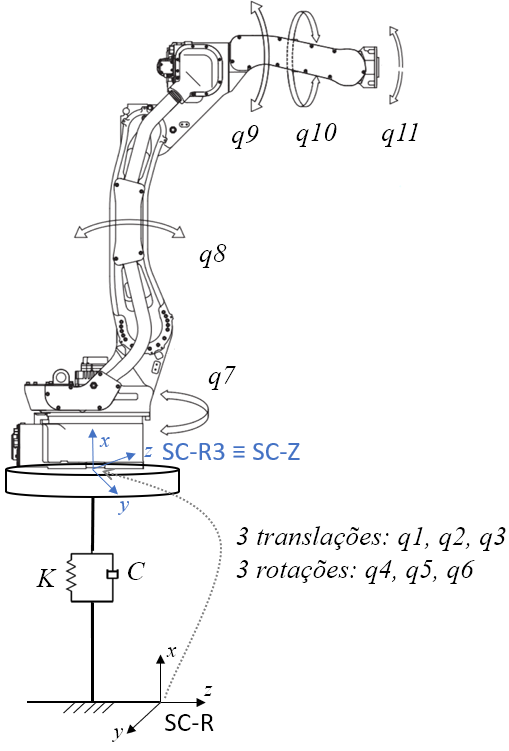
\includegraphics[width=0.45\textwidth]{figs/esq_acoplado}
 	\caption{Novas coordenadas generalizadas do modelo MBS acoplado}
 	\label{fig::esq_acoplado}
\end{figure}

Para este sistema acoplado, é empregado o mesmo procedimento das
seções~\ref{sec::robo} e \ref{sec::base} para se deduzir as equações de
movimento, pelo Método de Kane e utilizando as rotinas do Sophia-Maple. A
principal diferença está na interface entre o robô e a base, em SC-R3/SC-Z.
Do ponto de vista do modelo do manipulador, o pedestal (ou corpo Z) que
antes não era considerado na dinâmica do sistema por estar fixo no referencial
inercial, agora irá sofrer os esforços externos, oriundos da conexão com a base
e também forças de inércia. O equilíbrio das forças externas na interface entre
os dois sistemas é apresentado no diagrama de corpo livre da
Figura~\ref{fig::dcl_interface}. Os outros elos do manipulador aparecem
sombreados, apenas como referência.

\begin{figure}[h]
	\centering 
 	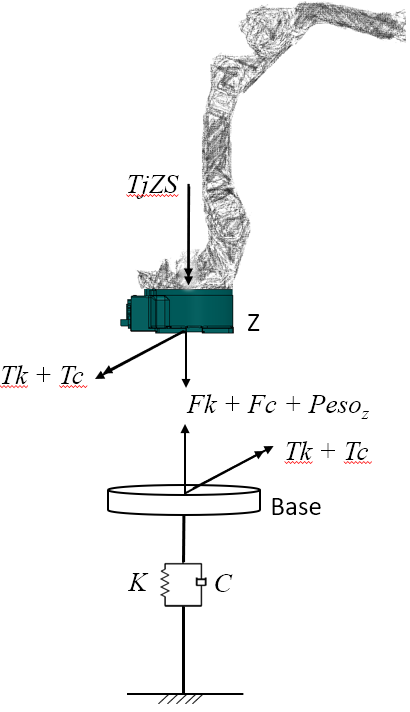
\includegraphics[width=0.40\textwidth]{figs/dcl_interface}
 	\caption{Diagrama de corpo livre da interface entre o pedestal do robô e a
 	base}
 	\label{fig::dcl_interface}
\end{figure}

Verifica-se que a rigidez e amortecimento da base atuam como forças e momentos
externos no robô. A expressão que define as forças externas que atuam no corpo
Z, que no modelo desacoplado apresentava apenas o peso do corpo, agora é:
%
\begin{equation}
	\mathbf{Fex}_Z = \mathbf{Peso}_Z - \mathbf{Fk} - \mathbf{Fc}
\end{equation}
%
Da mesma forma, a nova expressão para os momemntos externos que atuam no corpo
Z, que antes considerava apenas o torque da junta ZS, torna-se:
%
\begin{equation}
	\mathbf{Mex}_Z = -\mathbf{TjZS} - \mathbf{Tk} - \mathbf{Tc}
\end{equation}
%

Estas expressões são perfeitamente equivalentes às apresentadas na
equação~\ref{eq::fexm}, que tratava o corpo sobre a base como uma massa M
qualquer. Portanto, é de se notar que as expressões já desenvolvidas para o
cálculo dos modelos desacoplados do robô e da base, são perfeitamente
equivalentes às do modelo acoplado, sendo necessário apenas fazer a mudança das
coordenadas generalizadas e corrigir a indicação dos corpos, para refletir o
novo modelo.

O aumento do número de graus de liberdade, de 6 para 11, aliado a um novo
conjunto de forças externas, causa um grande aumento de complexidade no
cálculo algébrico das equações de movimento. Para se ter uma ideia, o novo custo
do sistema de equações de movimento do modelo acoplado robô e base, tem a
seguinte estrutura.
%
$$ 72220~\textit{additions} + 617367~\textit{multiplications} + 409552~
\textit{functions} $$
%


\subsection{Robô sobre base rígida}

A base é considerada rígida quando os deslocamentos devido a elasticidade de
sua estrutura causam erros desprezíveis de trajetória do robô. Ou seja erros
muito pequenos de posição, velocidade e orientação do seu efetuador. Uma base
rígida portanto seria um caso especial do modelo acoplado robô e base, tal que a
matriz de rigidez apresentasse valores muito elevados. No entanto, a medida que
se aumenta a rigidez da base, o modelo converge para o caso do sistema
desacoplado, no sentido que a rigidez é tão alta que os graus de liberdade
oferecidos pela base resultam em movimentos desprezíveis.

Entende-se que do cálculo da cinemática inversa, é definida a trajetória ideal,
que fornece os parâmetros de posição, velocidade e orientação exatos que se
deseja realizar.
Porém, a cinemática inversa fornece apenas um dado de entrada ao modelo
dinâmico, tal que a trajetória real será consequência da inércia do sistema e da
eficácia do controlador PID. A diferença entre a trajetória resultante e a
fornecida é classificada como erro de trajetória, onde os erros são apresentados
em termos de posição, velocidade e orientação. Logo, é de se esperar que, se o robô
é bem projetado e seu controle bem determinado, os erros apresentados estarão
dentro de uma faixa de erro aceitável. Na seção~\ref{sec::insitu} foram
apresentados os requisitos para o processo de revestimento por asperção
térmica. Este processo é utilizado para exemplificar a utilização do método
para alguns casos de bases flexíveis, na seção~\ref{sec::casos}.

O modelo do robô sobre base rígida será portanto utilizado para descrever uma
trajetória de referência, ou seja, resultado puramente da dinâmica do robô,
desconsiderando qualquer grau de liberdade da base. Seus resultados servirão de
referência, portanto, para comparar com os do manipulador sobre bases flexíveis.

\subsection{Robô sobre base flexível}

Quando a base possui pouca rigidez, e havendo deslocamentos consideráveis devido
à dinâmica do robô, o modelo acoplado deve ser utilizado. A mesma trajetória do
modelo desacoplado, é fornecida e obtém-se os novos resultados. Calcula-se então
os erros de posição, velocidade e orientação, e compara-se com os resultados do
outro modelo.




% -.~.-.~.-.~.-.~.-.~.-.~.-.~.-.~.-.~.-.~.-.~.-
\section{Casos aplicados}\label{sec::casos}

É apresentada a aplicação do método para alguns casos propostos. São definidas 2
trajetórias, diferentes em requisitos de velocidade, passo e orientação. Estas
trajetórias são aplicadas ao modelo de base rígida, que fornece os resultados de
referência, e depois aplicadas no modelo acoplado com base flexível. Os casos de
base são analisados para 4 versões, da mais rígida à mais flexível, cujos modelos são:
%
\begin{enumerate*}[label=\emph{\roman*})]
	\item base rígida;
	\item base de testes;
	\item base modular PRP;
	\item base telescópica PRPP.
\end{enumerate*}
%
Os resultados são analisados e discutidos no
Capítulo~\ref{cap::resultados}.

De maneira geral, o método para análise de casos segue o seguiunte fluxo de
tarefas:
%
\begin{enumerate}
  \item Definir a cinemática direta do manipulador robótico utilizado;
  \item Definir a trajetória, e calcular sua função pela cinemática inversa;
  \item Calcular a matriz de rigidez da base por Análise por Elementos Finitos;
  \item Fornecer a matriz de amortecimento da base;
  \item Simular a função calculada da trajetória no MBS acoplado;
  \item Calcular os erros de trajetória.
\end{enumerate}

Em todos os casos, o manipulador utilizado é o MOTOMAN MH12, que foi definido
no modelo do robô. As seções a seguir definem as trajetórias e os parâmetros
de rigidez e amortecimento dos casos de bases propostos.

\subsection{Trajetórias do efetuador}

Para exemplificar o uso do método, são propostas 2 trajetórias de simulação de
revestimento de uma superfície plana, em zigue-zague. Este tipo de trajetória
corresponde a uma tarefa que requer precisão de posição, velocidade e
orientação, a fim de garantir a qualidade do revestimento.

A primeira tarefa consiste em cobrir uma superfície no plano $xz$, com
velocidade constante de $40~m/min$ e passo entre paralelos de $3~mm$. A segunda
tarefa é cobrir uma superfície no plano $yx$ com velocidade de $30~m/min$ e
passo de $10~mm$.

Os cartões a seguir resumem as informações referentes às trajetórias de cada
tarefa a ser simulada e as Figuras~\ref{fig::traj1_subf} e \ref{fig::traj2_subf}
apresentam o traçado de cada trajetória no plano correspondente e a
representação no ambiente 3D com o robô no início do primeiro paralelo.
%
\newline
\begin{tcolorbox}
[colframe=black!75!white, colback=white, title = Tarefa 1 -- Plano xz] 
  \textbf{Área:} $(600 \times 12)~mm^2$ \\
  \textbf{Ponto inicial:} $\mathbf{p}_f = [0,700,~1,238,~-0,600]$ \\
  \textbf{Orientação:} $\boldsymbol{\Phi}_{f} = [0,~0,~0]$ \\
  \textbf{Passo:} $3~mm$ \\
  \textbf{Número de paralelos:} 4 \\
  \textbf{Velocidade da ferramenta:} $40~m/min$
\end{tcolorbox}
%
\begin{figure}[h]
    \centering
    \begin{subfigure}[b]{0.45\textwidth}
        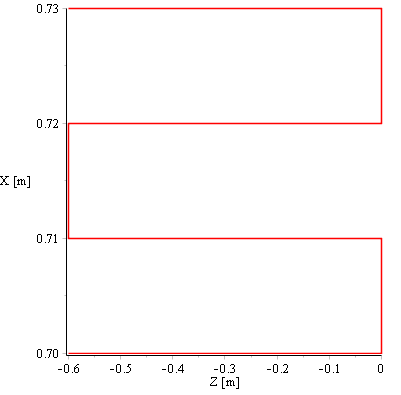
\includegraphics[width=\textwidth]{figs/traj1}
        \caption{Traçado da trajetória 1}
        \label{fig::traj1}
    \end{subfigure}
    \quad %add desired spacing between images, e. g. ~, \quad, \qquad, \hfill
    % etc.
      %(or a blank line to force the subfigure onto a new line)
    \begin{subfigure}[b]{0.49\textwidth}
        \includegraphics[width=\textwidth]{figs/traj1_3d}
        \caption{Trajetória 1 no ambiente 3D}
        \label{fig::traj1_3d}
    \end{subfigure}
    \caption{Trajetória referente à Tarefa 1}
    \label{fig::traj1_subf}
\end{figure}

%
\begin{tcolorbox}
[colframe=black!75!white, colback=white, title = Tarefa 2 -- Plano yz]
  \textbf{Área:} $(500 \times 40)~mm^2$ \\
  \textbf{Ponto inicial:} $\mathbf{p}_f = [-0,300,~0,600,~-0,500]$ \\
  \textbf{Orientação:} $\boldsymbol{\Phi}_{f} = [\pi/2,~\pi/2,~0]$ \\
  \textbf{Passo:} $10~mm$ \\
  \textbf{Número de paralelos:} 4 \\
  \textbf{Velocidade da ferramenta:} $30~m/min$
\end{tcolorbox}
%
\begin{figure}[h!]
    \centering
    \begin{subfigure}[b]{0.50\textwidth}
        \includegraphics[width=\textwidth]{figs/traj2}
        \caption{Traçado da trajetória 2}
        \label{fig::traj2}
    \end{subfigure}
    \quad %add desired spacing between images, e. g. ~, \quad, \qquad, \hfill
    % etc.
      %(or a blank line to force the subfigure onto a new line)
    \begin{subfigure}[b]{0.45\textwidth}
        \includegraphics[width=\textwidth]{figs/traj2_3d}
        \caption{Trajetória 2 no ambiente 3D}
        \label{fig::traj2_3d}
    \end{subfigure}
    \caption{Trajetória referente à Tarefa 2}
    \label{fig::traj2_subf}
\end{figure}


\subsection{Base rígida}

Neste caso, como já foi citado, o modelo MBS utilizado será o desacoplado,
apenas do robô. O sistema tem apenas os 5 graus de liberdade associados às juntas do
manipulador.

Os resultados da simulação para o caso da base rígida é apresentado na
seção~\ref{sec::res_rigida} e são utilizados como referência para comparação
com os outros modelos de base.


\subsection{Base de testes} \label{sec::base_testes}

Esta é a base foi construída para testes do projeto EMMA e consiste em uma
plataforma metálica e modular, com trilho e placa para fixação do robô a uma
altura de aproximadamente $600~mm$ do piso. A
Figura~\ref{fig::estrut_modelo_fisico} apresentou uma fotografia da base
construída, sem o robô.
A estrutura é formada por perfis leves de alumínio estrutural e o trilho é
composto por perfis de aço inoxidável. Patins de rolamentos
acoplam a placa de fixação de alumínio aos trilhos paralelos na estrutura.

Na seção~\ref{sec::aef} esta base foi utilizada para apresentar o modelo para
Análise por Elementos Finitos, que forneceu sua matriz de rigidez.
%
\begin{equation*}
	K =
\begin{pmatrix}
941537	&	0	&	0	&	0	&	0	&	0 \\
0	&	130543	&	0	&	0	&	0	&	-24981 \\
0	&	0	&	262149	&	0	&	5757	&	0 \\
0	&	0	&	0	&	57019	&	0	&	0 \\
0	&	0	&	5757	&	0	&	119561	&	0 \\
0	&	-24981	&	0	&	0	&	0	&	97595 \\
\end{pmatrix}
\end{equation*}
%
E na seção~\ref{sec::experimento} foi detalhado o experimento realizado com o
modelo físico, a fim de determinar os parâmetros de Rayleigh para a matriz de
amortecimento. 
%
\begin{align*}
	\alpha &= 0,04489 \\
	\beta &= 0.00006907
\end{align*}
%

Calcula-se, portanto, a seguinte matriz de amortecimento:
%
\begin{equation}
	C =
\begin{pmatrix}
65042	&	0		&	0		&	0		&	0		&	0		\\
0		&	9024	&	0		&	0		&	0		&	-1726	\\
0		&	0		&	18115	&	0		&	397	 	&	0		\\
0		&	0		&	0		&	3939 	&	0		&	0		\\
0		&	0		&	397		&	0		&	8260 	& 	0		\\
0		&	-1726	&	0		&	0		&	0		&	6744
\end{pmatrix}
\end{equation}
%
Valores em $kg/s$ e $kg~m/s$. 

Os resultados das tarefas para esta base são apresentados na
seção~\ref{sec::res_testes}.


\subsection{Base modular PRP} \label{sec::base_prp}

Esta base consiste em um trilho primário e, sobreposto a este, um trilho
secundário, utilizados para posicionar o manipulador dentro do ambiente de uma
turbina.
Uma plataforma de rotação permite que o trilho secundário forme qualquer ângulo
em relação ao primário. Sobre o trilho secundário corre a placa de fixação do
robô. Portanto, esta base é classificada como Prismática-Rotacional-Prismática
ou PRP, por fornecer tais graus de liberdade para o posicionamento do robô.

Na seção~\ref{sec::insitu} apresentou-se esta base no ambiente da turbina.
A Figura~\ref{fig::prp_cad} isola o modelo CAD da base com o robô. Na
configuração específica analisada, o trilho secundário forma $90^\circ$
em relação ao primário e a placa de fixação do robô a $1100~mm$ de distância da
plataforma de rotação.

\begin{figure}[h]
	\centering 
 	\includegraphics[width=0.80\textwidth]{figs/prp_cad}
 	\caption{Modelo CAD da base modular PRP}
 	\label{fig::prp_cad}
\end{figure}

Para determinação da matriz de rigidez, esta base é modelada para análise AEF. O
modelo é apresentado na Figura~\ref{fig::prp_fea}, onde os prinicipais
componentes são indicados.

\begin{figure}[h]
	\centering 
 	\includegraphics[width=0.95\textwidth]{figs/prp_fea}
 	\caption{Modelo para AEF da base modular PRP}
 	\label{fig::prp_fea}
\end{figure}

Os perfis, materiais e propriedades de seção do trilho e da estrutura são as
mesmas já descritas nas Figuras~\ref{fig::sectrans_bosch},
\ref{fig::sectrans_bosch} e na Tabela~\ref{tab::prop_mat} da base de testes. A
diferença é a introdução dos pés da estrutura e da plataforma de rotação. Os pés
são formados por tubos de alumínio de $50~mm$ de diâmetro externo e parede
$4~mm$, acoplados à estrutura por meio de abraçadeiras, podendo ser
considerados engastados na estrutura principal.
As propriedades de seção estão descritas na Figura~\ref{fig::sectrans_pes}. O
material é o Alumínio EN-AW 6060 e suas propriedades também foram definidas na
Tabela~\ref{tab::prop_mat}.

\begin{figure}[h]
	\centering 
 	\includegraphics[width=0.80\textwidth]{figs/sectrans_pes}
 	\caption{Propriedades de seção trasnversal dos pés da estrutura}
 	\label{fig::sectrans_pes}
\end{figure}

A plataforma de rotação é formada por duas placas de alumínio, uma solidária ao
trilho primário e a outra ao trilho secundário, unidas por um mancal de
rolamento do tipo \textit{slewing-ring}. Devido a densidade e robustez, esta peça foi
construída com elementos rígidos no modelo para AEF. Logo transmitem forças e
momentos, mas não se deforma. Da mesma forma a placa de fixação é considerada
rígida e possui um ponto onde virtualmente está acoplado o robô e por onde as
cargas são aplicadas.

As restrições são do tipo engaste e aplicadas às extremidades do pés de apoio da
estrutura. Os deslocamentos prescritos são então aplicados em 6 casos,
exatamente como foi realizado no exemplo da seção~\ref{sec::base}, de acordo com a
Tabela~\ref{tab::casoscarreg}. A matriz de rigidez desta versão da base é então
obtida dos resultados da análise AEF:

%
\begin{equation}
	K = 
\begin{pmatrix}
311723	&	-194	&	-4274	&	-161	&	47454	&	-16 \\
-194	&	15416	&	122	&	-12199	&	-85	&	-2100 \\
-4274	&	122	&	18059	&	1374	&	59	&	5 \\
-161	&	-12199	&	1374	&	13193	&	39	&	1379 \\
47454	&	-85	&	59	&	39	&	18643	&	-7 \\
-16	&	-2100	&	5	&	1379	&	-7	&	18698
\end{pmatrix}
\end{equation}
%
Valores em $kN/m$ e $kNm/rad$.

Para a matriz de amortecimento, seria necessário o ensaio experimental da
estrutura. Como ainda não existe o modelo físico desta vesão da base, os valores
de $\alpha$ e $\beta$ serão estimados. Pode-se considerar uma estimativa
razoável, devido à semelhança de materiais e peças, $\alpha = 0$ e $\beta = 5
\times 10^{-5}$. Portanto, a matriz de amortecimento torna-se:
%
\begin{equation}
	C = 
\begin{pmatrix}
2136	&	-29		&	-179	&	-8		&	912		&	-4 	\\
-29		&	450 	&	5		&	-389	&	-12		&	-41 \\
-179	&	5		&	471		&	70		&	-35		&	1 	\\
-8		&	-389	&	70		&	446		&	3		&	36	\\
912		&	-12		&	-35		&	3		&	468		&	-2	\\
-4		&	-41		&	1		&	36		&	-2		&	293	\\
\end{pmatrix}
\end{equation}
%
Valores em $kg/s$ e $kg~m/s$.

Os resultados das tarefas simuladas nesta base são apresentados na
seção~\ref{sec::res_prp}.



\subsection{Base telescópica PRPP} \label{sec::base_prpp}

Um último caso de base a ser analisado busca apresentar uma versão muito
flexível, isto é, embora capaz de suportar os esforços com boa margem de
segurança, oferece deslocamentos inaceitáveis para a realização da tarefa.

Esta base foi apresentada na seção~\ref{sec::insitu}, na
Figura~\ref{fig::base_telesc_turbina}. Por decisão conservadora, decidiu-se não
utilizá-la como solução, devido a um estudo preliminar de rigidez. Na época
ainda não havia o método proposto neste trabalho e será utilizado agora para
verificar a resposta dinâmica desta base para as tarefas de revestimento.

A base consiste em uma estrutura telescópica, que oferece graus de liberdade do
tipo Prismático-Rotacional-Prismático-Prismático (PRPP), utilizados para
posicionamento do robô.
A Figura~\ref{fig::base_telesc} apresenta modelo CAD da configuração retraída, à
esquerda, e estendida à direita.

\begin{figure}[h]
	\centering 
 	\includegraphics[width=0.70\textwidth]{figs/base_telesc}
 	\caption{Base telescópica PRPP para acesso pela escotilha superior}
 	\label{fig::base_telesc}
\end{figure}

Os itens numerados correspondem à: 
%
\begin{enumerate*}[label=(\arabic*)]
  \item atuador linear do tipo sem-fim-coroa;
  \item base fixa na escotilha;
  \item braço prismático \#1;
  \item braço prismático \#2;
  \item atuadores lineares;
  \item junta de rotação;
  \item braço prismático \#3.
\end{enumerate*}
%

O robô é fixado na extremidade do braço prismático \#3. Embora na solução
original fosse utilizado um robô mais leve, será verificada a resposta
deste caso para o manipulador MH12.

Para determinar a matriz de rigidez desta base, é criado seu modelo para AEF.
Será considerada a configuração em que as juntas prismáticas estão totalmente
estendidas e a rotacional formando um ângulo de $90^\circ$. A
Figura~\ref{fig::base_telesc_fea} apresenta este modelo indicando os prinicipais
componentes.

\begin{figure}[h]
	\centering 
 	\includegraphics[width=0.45\textwidth]{figs/base_telesc_fea}
 	\caption{Modelo da base telescópica PRPP para AEF}
 	\label{fig::base_telesc_fea}
\end{figure}

Os componentes foram modelados como elementos de viga onde os braços prismáticos
são formados por tubos de seção circular, padrão Schedule.
As propriedades de seção transversal utilizadas na análise são apresentadas na
Tabela~\ref{tab::sectrans_schedules}. 
%
\begin{table}[h!]
\centering
\caption{Propriedades de seção transversal dos componentes da base PRPP}
\label{tab::sectrans_schedules}
\begin{tabular}{@{}llccc@{}}
\toprule
\textbf{Propriedade}   &           & \textbf{Base fixa} & \textbf{Braços 1 e 2} & \textbf{Braço 3} \\ \midrule
Diâmetro nom.          & [$pol$] & 10                 & 8                     & 6                \\
Padrão Schedule        &           & SCH 40             & SCH40                 & SCH 40           \\
Área de seção          & [$mm^2$]  & 7,68E3             & 5,42E3                & 3,60E3           \\
Inércia polar, J1      & [$mm^4$]  & 1,34E8             & 6,04E7               
& 2,34E7           \\
Momento de Inércia, I2 & [$mm^4$]  & 6,70E7             & 3,02E7                & 1,17E7           \\
Momento de Inércia, I3 & [$mm^4$]  & 6,70E7             & 3,02E7                & 1,17E7           \\
Módulo de seção, S2    & [$mm^3$]  & 4,90E5             & 2,75E5                & 1,39E5           \\
Módulo de seção, S3    & [$mm^3$]  & 4,90E5             & 2,75E5                & 1,39E5           \\ \bottomrule
\end{tabular}
\end{table}
%

Os tubos são de aço ASTM A36, e suas propriedades de material são apresentadas
na Tabela~\ref{tab::astma36}.
%
\begin{table}[h!]
\centering
\caption{Propriedades de material do aço ASTM A36}
\label{tab::astma36}
\begin{tabular}{@{}llc@{}}
\toprule
\textbf{Propriedade}   & \textbf{}  & \textbf{ASTM A36} \\ \midrule
Densidade              & {[}g/cc{]} & 7,85              \\
Módulo de Elasticidade & {[}GPa{]}  & 200               \\
Coeficiente de Poison  & {[}1{]}    & 0,29              \\
Tensão de Escoamento   & {[}MPa{]}  & 248               \\
Resistência à tração   & {[}MPa{]}  & 400               \\ \bottomrule
\end{tabular}
\end{table}
%

É considerada restrição do tipo engastada no topo da base fixa, representando
sua fixação na entrada da escotilha. Os 6 casos de carregamento e restições são
então aplicados no ponto de fixação do robô, novamente de acordo com a
Tabela~\ref{tab::casoscarreg}.

O resultado para a matriz de rigidez desta base, obtido pelas simulações por
AEF é apresentado na equação~\ref{eq::res_rigidez_prpp}.

%
\begin{equation} \label{eq::res_rigidez_prpp}
	K = 
\begin{pmatrix}
148768	&	-52549	&	0	&	0	&	0	&	10299 \\
-52549	&	57244	&	0	&	0	&	0	&	-21023 \\
0	&	0	&	26634	&	1984	&	12700	&	0 \\
0	&	0	&	1984	&	2926	&	946	&	0 \\
0	&	0	&	12700	&	946	&	9126	&	0 \\
10299	&	-21023	&	0	&	0	&	0	&	11866
\end{pmatrix}
\end{equation}
%
Valores da matriz em $kN/m$ e $kNm/rad$.

Novamente, não é disponível esta versão para ensaio experimental, portanto os
parâmetros $\alpha$ e $\beta$ para formar a matriz de amortecimento são
estimados.
Sejam os valores $\alpha = 0$ e $\beta = 5 \times 10^{-5}$, a matriz de
amortecimento será:
%
\begin{equation} \label{eq::res_amortecimento_prpp}
	C = 
\begin{pmatrix}
7438	&	-2627	&	0	&	0	&	0	&	515 \\
-2627	&	2862	&	0	&	0	&	0	&	-1051 \\
0	&	0	&	1332	&	99	&	635	&	0 \\
0	&	0	&	99	&	146	&	47	&	0 \\
0	&	0	&	635	&	47	&	456	&	0 \\
515	&	-1051	&	0	&	0	&	0	&	593
\end{pmatrix}
\end{equation}
%
Valores da matriz em $kg/s$ e $kg~m/s$.


  \chapter{Resultados e Discussões} \label{cap::resultados}

Os resultados das simulações de cada tarefa proposta são apresentados nas
seções~\ref{sec::resultados_t1} e \ref{sec::resultados_t2} para os seguintes
casos de base:
%
\begin{enumerate*}[label=\emph{\roman*})]
	\item base rígida;
	\item base de testes;
	\item base modular PRP;
	\item base telescópica PRPP.
\end{enumerate*}
%

Em todos os casos são avaliados os erros de posicionamento, velocidade e
orientação da ferramenta, ao longo de toda a tarefa. Na
seção~\ref{sec::comparacao} são comparados os resultados das tarefas para as
diferentes bases.

% -.~.-.~.-.~.-.~.-.~.-.~.-.~.-.~.-.~.-.~.-.~.-
\section{Resultados de simulação da Tarefa 1} \label{sec::resultados_t1}


\subsection{Base rígida -- Tarefa 1} \label{sec::res_rigida}

Seguem os resultados do modelo de base rígida que utiliza o modelo MBS --
Robô.
A Figura~\ref{fig::t1_anima3D_base_rig} apresenta o resultado da simulação no ambiente
3D para a Tarefa 1.

\begin{figure}[h!]
	\centering 
 	\includegraphics[width=0.50\textwidth]{figs/t1_anima3D_base_rig}
 	\caption{Simulação no ambiente 3D para a Tarefa 1}
 	\label{fig::t1_anima3D_base_rig}
\end{figure}

Estes resultados representam uma referência para posterior comparação com os
resultados obtidos para o modelo MBS acoplado.

\subsubsection{Posição da ferramenta}

Os resultados de simulação da posição da ponta da ferramenta para Tarefa 1 são
apresentados a seguir. A Figura~\ref{fig::t1_posf_base_rig} fornece o valor de
cada coordenada $x, y, z$ no referencial inercial (linha cheia) e também o valor
de referência (linha tracejada), fornecido pela cinemática inversa. A
Figura~\ref{fig::t1_erroposf_base_rig} fornece o erro de posição, ou seja, a
diferença entre o valor de referência dado pela cinemática inversa e o efetivo,
de cada coordenada, assim como o erro absoluto (linha tracejada).

\begin{figure}[h!]
	\centering 
 	\includegraphics[width=0.80\textwidth]{figs/t1_posf_base_rig}
 	\caption{Posições das coordenadas da ferramenta para base rígida -- Tarefa 1}
 	\label{fig::t1_posf_base_rig}
\end{figure}

\begin{figure}[h!]
	\centering 
 	\includegraphics[width=0.80\textwidth]{figs/t1_erroposf_base_rig}
 	\caption{Erro de posição da ferramenta para base rígida -- Tarefa 1}
 	\label{fig::t1_erroposf_base_rig}
\end{figure}


\subsubsection{Trajetória da ferramenta}

A Figura~\ref{fig::t1_traj_base_rig} apresenta a trajetória da ferramenta
projetada no plano $xz$ (linha cheia) e a trajetória de referência (linha
tracejada).
Note-se que os eixos não estão na mesma escala, para facilitar a visualização da
trajetória.

\begin{figure}[h!]
	\centering 
 	\includegraphics[width=0.80\textwidth]{figs/t1_traj_base_rig}
 	\caption{Trajetória projetada no plano $zx$ para base rígida -- Tarefa 1}
 	\label{fig::t1_traj_base_rig}
\end{figure}


\subsubsection{Velocidade da ferramenta}

São apresentados os gráficos da velocidade da ponta da ferramenta (linhas
cheias) e as velocidades de referência dadas pela cinemática inversa (linhas
tracejadas), na Figura~\ref{fig::t1_velf_base_rig}. Na
Figura~\ref{fig::t1_errovelf_base_rig} os erros em relação a velocidade de
referência, no referencial inercial.

\begin{figure}[h!]
	\centering 
 	\includegraphics[width=0.80\textwidth]{figs/t1_velf_base_rig}
 	\caption{Velocidades das coordenadas da ferramenta para base rígida -- Tarefa 1}
 	\label{fig::t1_velf_base_rig}
\end{figure}

\begin{figure}[h!]
	\centering 
 	\includegraphics[width=0.80\textwidth]{figs/t1_errovelf_base_rig}
 	\caption{Erro de velocidade da ferramenta para base rígida --
 	Tarefa 1}
 	\label{fig::t1_errovelf_base_rig}
\end{figure}


\subsubsection{Orientação da ferramenta}

O erro de orientação da ferramenta é resultado da matriz de rotação entre o
referencial inercial e a orientação do pulso do robô, em função dos ângulos de
Euler, para a orientação desejada. Faz-se uma transformação da matriz de rotação
em eixo e ângulo, de acordo com as equações~\ref{eq::ang_erro} e
\ref{eq::eixo_erro}. A Figura~\ref{fig::t1_erroori_base_rig} apresenta o
erro de orientação, representado pelo ângulo $\theta$, para a Tarefa 1.

\begin{figure}[h!]
	\centering 
 	\includegraphics[width=0.80\textwidth]{figs/t1_erroori_base_rig}
 	\caption{Erro de orientação da ferramenta para base rígida -- Tarefa
 	1}
 	\label{fig::t1_erroori_base_rig}
\end{figure}



\subsection{Base de testes -- Tarefa 1} \label{sec::res_testes}

Apresenta-se os resultados das trajetórias considerando o manipulador montado
sobre a base de testes, da seção~\ref{sec::base_testes}, realizando a Tarefa 1.

\subsubsection{Posição do ponto virtual}

O reusltado da Figura~\ref{fig::t1_q123456_base_testes} apresenta a variação das
coordenadas generalizadas $q1$ a $q3$, referentes às translações, e $q4$ a $q6$,
referentes às rotações do ponto virtual de acoplamento base e robô. A
Figura~\ref{fig::t1_pvirtural_base_testes} ilustra o rastro da posição do ponto
virtual (origem do robô) no ambiente 3D.

\begin{figure}[h]
    \centering
    \begin{subfigure}[b]{0.48\textwidth}
        \includegraphics[width=\textwidth]{figs/t1_q123_base_testes}
        \caption{Deslocamentos do ponto virtual}
        \label{fig::t1_q123_base_testes}
    \end{subfigure}
    \quad %add desired spacing between images, e. g. ~, \quad, \qquad, \hfill
    % etc.
      %(or a blank line to force the subfigure onto a new line)
    \begin{subfigure}[b]{0.48\textwidth}
        \includegraphics[width=\textwidth]{figs/t1_q456_base_testes}
        \caption{Rotações do ponto virtual}
        \label{fig::t1_q456_base_testes}
    \end{subfigure}
    \caption{Variações de posição e orientação da base de testes -- Tarefa 1}
    \label{fig::t1_q123456_base_testes}
\end{figure}

\begin{figure}[h!]
	\centering 
 	\includegraphics[width=0.70\textwidth]{figs/t1_pvirtural_base_testes}
 	\caption{Rastro da posição do ponto virtual -- Tarefa 1}
 	\label{fig::t1_pvirtural_base_testes}
\end{figure}


\subsubsection{Posição da ferramenta}

A Figura~\ref{fig::t1_posf_base_testes} fornece as posições efetiva (linhas
cheias) e ideal (linhas tracejadas). E a
Figura~\ref{fig::t1_erroposf_base_testes} o erro de cada coordenada, com
respeito ao referencial inercial.

\begin{figure}[h!]
	\centering 
 	\includegraphics[width=0.80\textwidth]{figs/t1_posf_base_testes}
 	\caption{Posições das coordenadas da ferramenta para base de testes -- Tarefa
 	1}
 	\label{fig::t1_posf_base_testes}
\end{figure}

\begin{figure}[h!]
	\centering 
 	\includegraphics[width=0.80\textwidth]{figs/t1_erroposf_base_testes}
 	\caption{Erro de posição da ferramenta para base de testes -- Tarefa 1}
 	\label{fig::t1_erroposf_base_testes}
\end{figure}


\subsubsection{Trajetória da ferramenta}

A Figura~\ref{fig::t1_traj_base_testes} apresenta a trajetória da ferramenta
projetada no plano $xz$ (linha cheia) e a trajetória de referência (linha
tracejada).
Note-se que os eixos não estão na mesma escala, para facilitar a visualização da
trajetória.

\begin{figure}[h!]
	\centering 
 	\includegraphics[width=0.70\textwidth]{figs/t1_traj_base_testes}
 	\caption{Trajetória projetada no plano $zx$ para base de testes -- Tarefa 1}
 	\label{fig::t1_traj_base_testes}
\end{figure}


\subsubsection{Velocidade da ferramenta}

São apresentados os gráficos da velocidade da ponta da ferramenta (linhas
cheias) e as velocidades de referência dadas pela cinemática inversa (linhas
tracejadas), na Figura~\ref{fig::t1_velf_base_testes} e na
Figura~\ref{fig::t1_errovelf_base_testes} os erros em relação a velocidade de
referência, no referencial inercial.

\begin{figure}[h!]
	\centering 
 	\includegraphics[width=0.80\textwidth]{figs/t1_velf_base_testes}
 	\caption{Velocidades das coordenadas da ferramenta base de testes --
 	Tarefa 1}
 	\label{fig::t1_velf_base_testes}
\end{figure}

\begin{figure}[h!]
	\centering 
 	\includegraphics[width=0.80\textwidth]{figs/t1_errovelf_base_testes}
 	\caption{Erro de velocidade da ferramenta para base de testes --
 	Tarefa 1}
 	\label{fig::t1_errovelf_base_testes}
\end{figure}


\subsubsection{Orientação da ferramenta}

A Figura~\ref{fig::t1_erroori_base_testes} apresenta o erro de orientação,
representado pelo ângulo $\theta$.

\begin{figure}[h!]
	\centering 
 	\includegraphics[width=0.80\textwidth]{figs/t1_erroori_base_testes}
 	\caption{Erro de orientação da ferramenta para base de testes -- Tarefa
 	1}
 	\label{fig::t1_erroori_base_testes}
\end{figure}



\subsection{Base modular PRP -- Tarefa 1} \label{sec::res_prp}

Apresenta-se os resultados das trajetórias considerando o manipulador montado
sobre a base modular PRP, da seção~\ref{sec::base_prp}, realizando a Tarefa 1.

\subsubsection{Posição do ponto virtual}

O reusltado da Figura~\ref{fig::t1_q123456_base_prp} apresenta a variação das
coordenadas generalizadas $q1$ a $q3$, referentes às translações, e $q4$ a $q6$,
referentes às rotações do ponto virtual de acoplamento base e robô. A
Figura~\ref{fig::t1_pvirtural_base_prp} ilustra o rastro da posição do ponto
virtual (origem do robô) no ambiente 3D.

\begin{figure}[h]
    \centering
    \begin{subfigure}[b]{0.48\textwidth}
        \includegraphics[width=\textwidth]{figs/t1_q123_base_prp}
        \caption{Deslocamentos do ponto virtual}
        \label{fig::t1_q123_base_prp}
    \end{subfigure}
    \quad %add desired spacing between images, e. g. ~, \quad, \qquad, \hfill
    % etc.
      %(or a blank line to force the subfigure onto a new line)
    \begin{subfigure}[b]{0.48\textwidth}
        \includegraphics[width=\textwidth]{figs/t1_q456_base_prp}
        \caption{Rotações do ponto virtual}
        \label{fig::t1_q456_base_prp}
    \end{subfigure}
    \caption{Variações de posição e orientação da base PRP -- Tarefa 1}
    \label{fig::t1_q123456_base_prp}
\end{figure}

\begin{figure}[h!]
	\centering 
 	\includegraphics[width=0.70\textwidth]{figs/t1_pvirtural_base_prp}
 	\caption{Rastro da posição do ponto virtual -- Tarefa 1}
 	\label{fig::t1_pvirtural_base_prp}
\end{figure}


\subsubsection{Posição da ferramenta}

A Figura~\ref{fig::t1_posf_base_prp} fornece as posições efetiva (linhas cheias)
e ideal (linhas tracejadas). E a Figura~\ref{fig::t1_erroposf_base_prp} o erro
de cada coordenada, com respeito ao referencial inercial.

\begin{figure}[h!]
	\centering 
 	\includegraphics[width=0.80\textwidth]{figs/t1_posf_base_prp}
 	\caption{Posições das coordenadas da ferramenta para base PRP -- Tarefa
 	1}
 	\label{fig::t1_posf_base_prp}
\end{figure}

\begin{figure}[h!]
	\centering 
 	\includegraphics[width=0.80\textwidth]{figs/t1_erroposf_base_prp}
 	\caption{Erro de posição da ferramenta para base PRP -- Tarefa 1}
 	\label{fig::t1_erroposf_base_prp}
\end{figure}


\subsubsection{Trajetória da ferramenta}

A Figura~\ref{fig::t1_traj_base_prp} apresenta a trajetória da ferramenta
projetada no plano $xz$ (linha cheia) e a trajetória de referência (linha
tracejada).
Note-se que os eixos não estão na mesma escala, para facilitar a visualização da
trajetória.

\begin{figure}[h!]
	\centering 
 	\includegraphics[width=0.70\textwidth]{figs/t1_traj_base_prp}
 	\caption{Trajetória projetada no plano para base PRP -- Tarefa 1}
 	\label{fig::t1_traj_base_prp}
\end{figure}


\subsubsection{Velocidade da ferramenta}

São apresentados os gráficos da velocidade da ponta da ferramenta (linhas
cheias) e as velocidades de referência dadas pela cinemática inversa (linhas
tracejadas), na Figura~\ref{fig::t1_velf_base_prp} e na
Figura~\ref{fig::t1_errovelf_base_prp} os erros em relação a velocidade de
referência, no referencial inercial.

\begin{figure}[h!]
	\centering 
 	\includegraphics[width=0.80\textwidth]{figs/t1_velf_base_prp}
 	\caption{Velocidades das coordenadas da ferramenta base PRP --
 	Tarefa 1}
 	\label{fig::t1_velf_base_prp}
\end{figure}

\begin{figure}[h!]
	\centering 
 	\includegraphics[width=0.80\textwidth]{figs/t1_errovelf_base_prp}
 	\caption{Erro de velocidade da ferramenta para base PRP --
 	Tarefa 1}
 	\label{fig::t1_errovelf_base_prp}
\end{figure}


\subsubsection{Orientação da ferramenta}

A Figura~\ref{fig::t1_erroori_base_prp} apresenta o erro de orientação,
representado pelo ângulo $\theta$.

\begin{figure}[h!]
	\centering 
 	\includegraphics[width=0.80\textwidth]{figs/t1_erroori_base_prp}
 	\caption{Erro de orientação da ferramenta para base PRP -- Tarefa
 	1}
 	\label{fig::t1_erroori_base_prp}
\end{figure}



\subsection{Base telescópica PRPP -- Tarefa 1} \label{sec::res_prpp}

\subsubsection{Posição do ponto virtual}

\subsubsection{Posição da ferramenta}

\subsubsection{Trajetória da ferramenta}

\subsubsection{Velocidade da ferramenta}

\subsubsection{Orientação da ferramenta}


\newpage
% -.~.-.~.-.~.-.~.-.~.-.~.-.~.-.~.-.~ TAREFA 2 ~.-.~.-.~.-.~.-.~.-.~.-.~.
\section{Resultados de simulação da Tarefa 2} \label{sec::resultados_t2}

\subsection{Base rígida -- Tarefa 2}

Seguem os resultados do modelo de base rígida que utiliza o modelo MBS --
Robô.
A Figura~\ref{fig::t2_anima3D_base_rig} apresenta o resultado da simulação no ambiente
3D para a Tarefa 2.

\begin{figure}[h!]
	\centering 
 	\includegraphics[width=0.50\textwidth]{figs/t2_anima3D_base_rig}
 	\caption{Simulação no ambiente 3D para a Tarefa 2}
 	\label{fig::t2_anima3D_base_rig}
\end{figure}


\subsubsection{Posição da ferramenta}

A Figura~\ref{fig::t2_posf_base_rig} fornece as posições efetiva (linhas cheias)
e ideal (linhas tracejadas). 

\begin{figure}[h!]
	\centering 
 	\includegraphics[width=0.80\textwidth]{figs/t2_posf_base_rig}
 	\caption{Posições das coordenadas da ferramenta para base rígida -- Tarefa 2}
 	\label{fig::t2_posf_base_rig}
\end{figure}

E a Figura~\ref{fig::t2_erroposf_base_rig} o erro
de cada coordenada, com respeito ao referencial inercial.

\begin{figure}[h]
	\centering 
 	\includegraphics[width=0.70\textwidth]{figs/t2_erroposf_base_rig}
 	\caption{Erro de posição da ferramenta para base rígida -- Tarefa 2}
 	\label{fig::t2_erroposf_base_rig}
\end{figure}


\subsubsection{Trajetória da ferramenta}

A Figura~\ref{fig::t2_traj_base_rig} apresenta a trajetória da ferramenta
projetada no plano $xy$ (linha cheia) e a trajetória de referência (linha
tracejada).

\begin{figure}[h]
	\centering 
 	\includegraphics[width=0.70\textwidth]{figs/t2_traj_base_rig}
 	\caption{Trajetória projetada no plano $yx$ para base rígida -- Tarefa 2}
 	\label{fig::t2_traj_base_rig}
\end{figure}


\subsubsection{Velocidade da ferramenta}

São apresentados os gráficos da velocidade da ponta da ferramenta (linhas
cheias) e as velocidades de referência dadas pela cinemática inversa (linhas
tracejadas), na Figura~\ref{fig::t2_velf_base_rig} e na
Figura~\ref{fig::t2_errovelf_base_rig} os erros em relação a velocidade de
referência, no referencial inercial.

\begin{figure}[h]
	\centering 
 	\includegraphics[width=0.85\textwidth]{figs/t2_velf_base_rig}
 	\caption{Velocidades das coordenadas da ferramenta base rígida -- Tarefa
 	2}
 	\label{fig::t2_velf_base_rig}
\end{figure}

\begin{figure}[h]
	\centering 
 	\includegraphics[width=0.85\textwidth]{figs/t2_errovelf_base_rig}
 	\caption{Erro de velocidade da ferramenta para base rígida -- Tarefa 2}
 	\label{fig::t2_errovelf_base_rig}
\end{figure}


\subsubsection{Orientação da ferramenta}

A Figura~\ref{fig::t2_erroori_base_rig} apresenta o erro de orientação da
ferramenta, representado pelo ângulo $\theta$.

\begin{figure}[h]
	\centering 
 	\includegraphics[width=0.80\textwidth]{figs/t2_erroori_base_rig}
 	\caption{Erro de orientação da ferramenta para base rígida -- Tarefa
 	2}
 	\label{fig::t2_erroori_base_rig}
\end{figure}


\subsection{Base de testes -- Tarefa 2}

\subsubsection{Posição do ponto virtual}

O reusltado da Figura~\ref{fig::t2_q123456_base_testes} apresenta a variação das
coordenadas generalizadas $q1$ a $q3$, referentes às translações, e $q4$ a $q6$,
referentes às rotações do ponto virtual de acoplamento base e robô. A
Figura~\ref{fig::t2_pvirtural_base_testes} ilustra o rastro da posição do ponto
virtual (origem do robô) no ambiente 3D.

\begin{figure}[h]
    \centering
    \begin{subfigure}[b]{0.48\textwidth}
        \includegraphics[width=\textwidth]{figs/t2_q123_base_testes}
        \caption{Deslocamentos do ponto virtual}
        \label{fig::t2_q123_base_testes}
    \end{subfigure}
    \quad %add desired spacing between images, e. g. ~, \quad, \qquad, \hfill
    % etc.
      %(or a blank line to force the subfigure onto a new line)
    \begin{subfigure}[b]{0.48\textwidth}
        \includegraphics[width=\textwidth]{figs/t2_q456_base_testes}
        \caption{Rotações do ponto virtual}
        \label{fig::t2_q456_base_testes}
    \end{subfigure}
    \caption{Variações de posição e orientação da base de testes -- Tarefa 2}
    \label{fig::t2_q123456_base_testes}
\end{figure}

\begin{figure}[h!]
	\centering 
 	\includegraphics[width=0.60\textwidth]{figs/t2_pvirtural_base_testes}
 	\caption{Rastro da posição do ponto virtual -- Tarefa 2}
 	\label{fig::t2_pvirtural_base_testes}
\end{figure}


\subsubsection{Posição da ferramenta}

A Figura~\ref{fig::t2_posf_base_testes} fornece as posições efetiva e ideal da
Tarefa 2, e a Figura~\ref{fig::t2_erroposf_base_testes} o erro de cada
coordenada, com respeito ao referencial inercial.

\begin{figure}[h!]
	\centering 
 	\includegraphics[width=0.75\textwidth]{figs/t2_posf_base_testes}
 	\caption{Posições das coordenadas da ferramenta para base de testes -- Tarefa
 	2}
 	\label{fig::t2_posf_base_testes}
\end{figure}

\begin{figure}[h!]
	\centering 
 	\includegraphics[width=0.75\textwidth]{figs/t2_erroposf_base_testes}
 	\caption{Erro de posição da ferramenta para base de testes -- Tarefa 2}
 	\label{fig::t2_erroposf_base_testes}
\end{figure}


\subsubsection{Trajetória da ferramenta}

A Figura~\ref{fig::t2_traj_base_testes} apresenta a trajetória da ferramenta
projetada no plano $xy$ (linha cheia) e a trajetória de referência (linha
tracejada).

\begin{figure}[h!]
	\centering 
 	\includegraphics[width=0.70\textwidth]{figs/t2_traj_base_testes}
 	\caption{Trajetória projetada no plano para base de testes -- Tarefa 2}
 	\label{fig::t2_traj_base_testes}
\end{figure}


\subsubsection{Velocidade da ferramenta}

A Figura~\ref{fig::t2_posf_base_testes} fornece as velocidades
efetivas e ideais . A Figura~\ref{fig::t2_erroposf_base_testes} o erro de cada
coordenada, com respeito ao referencial inercial.

\begin{figure}[h!]
	\centering 
 	\includegraphics[width=0.80\textwidth]{figs/t2_velf_base_testes}
 	\caption{Velocidades das coordenadas da ferramenta base de testes --
 	Tarefa 2}
 	\label{fig::t2_velf_base_testes}
\end{figure}

\begin{figure}[h!]
	\centering 
 	\includegraphics[width=0.80\textwidth]{figs/t2_errovelf_base_testes}
 	\caption{Erro de velocidade da ferramenta para base de testes --
 	Tarefa 2}
 	\label{fig::t2_errovelf_base_testes}
\end{figure}


\subsubsection{Orientação da ferramenta}

A Figura~\ref{fig::t2_erroori_base_testes} apresenta o erro de orientação da
ferramenta, representado pelo ângulo $\theta$.

\begin{figure}[h!]
	\centering 
 	\includegraphics[width=0.80\textwidth]{figs/t2_erroori_base_testes}
 	\caption{Erro de orientação da ferramenta para base de testes -- Tarefa
 	2}
 	\label{fig::t2_erroori_base_testes}
\end{figure}



\subsection{Base PRP -- Tarefa 2}

\subsubsection{Posição do ponto virtual}

O reusltado da Figura~\ref{fig::t2_q123456_base_prp} apresenta a variação das
coordenadas generalizadas $q1$ a $q3$, referentes às translações, e $q4$ a $q6$,
referentes às rotações do ponto virtual de acoplamento base e robô. A
Figura~\ref{fig::t2_pvirtural_base_prp} ilustra o rastro da posição do ponto
virtual (origem do robô) no ambiente 3D.

\begin{figure}[h]
    \centering
    \begin{subfigure}[b]{0.48\textwidth}
        \includegraphics[width=\textwidth]{figs/t2_q123_base_prp}
        \caption{Deslocamentos do ponto virtual}
        \label{fig::t2_q123_base_prp}
    \end{subfigure}
    \quad %add desired spacing between images, e. g. ~, \quad, \qquad, \hfill
    % etc.
      %(or a blank line to force the subfigure onto a new line)
    \begin{subfigure}[b]{0.48\textwidth}
        \includegraphics[width=\textwidth]{figs/t2_q456_base_prp}
        \caption{Rotações do ponto virtual}
        \label{fig::t2_q456_base_prp}
    \end{subfigure}
    \caption{Variações de posição e orientação da base PRP -- Tarefa 2}
    \label{fig::t2_q123456_base_prp}
\end{figure}

\begin{figure}[h!]
	\centering 
 	\includegraphics[width=0.70\textwidth]{figs/t2_pvirtural_base_prp}
 	\caption{Rastro da posição do ponto virtual -- Tarefa 2}
 	\label{fig::t2_pvirtural_base_prp}
\end{figure}


\subsubsection{Posição da ferramenta}

A Figura~\ref{fig::t2_posf_base_prp} fornece as posições efetiva e ideal da
Tarefa 2, e a Figura~\ref{fig::t2_erroposf_base_prp} o erro de cada
coordenada, com respeito ao referencial inercial.

\begin{figure}[h!]
	\centering 
 	\includegraphics[width=0.80\textwidth]{figs/t2_posf_base_prp}
 	\caption{Posições das coordenadas da ferramenta para base PRP -- Tarefa
 	2}
 	\label{fig::t2_posf_base_prp}
\end{figure}

\begin{figure}[h!]
	\centering 
 	\includegraphics[width=0.80\textwidth]{figs/t2_erroposf_base_prp}
 	\caption{Erro de posição da ferramenta para base PRP -- Tarefa 2}
 	\label{fig::t2_erroposf_base_prp}
\end{figure}


\subsubsection{Trajetória da ferramenta}

A Figura~\ref{fig::t2_traj_base_prp} apresenta a trajetória da ferramenta
projetada no plano $xy$ (linha cheia) e a trajetória de referência (linha
tracejada).

\begin{figure}[h!]
	\centering 
 	\includegraphics[width=0.80\textwidth]{figs/t2_traj_base_prp}
 	\caption{Trajetória projetada no plano para base PRP -- Tarefa 2}
 	\label{fig::t2_traj_base_prp}
\end{figure}


\subsubsection{Velocidade da ferramenta}

A Figura~\ref{fig::t2_posf_base_prp} fornece as velocidades
efetivas e ideais . A Figura~\ref{fig::t2_erroposf_base_prp} o erro de cada
coordenada, com respeito ao referencial inercial.

\begin{figure}[h!]
	\centering 
 	\includegraphics[width=0.80\textwidth]{figs/t2_velf_base_prp}
 	\caption{Velocidades das coordenadas da ferramenta base PRP --
 	Tarefa 2}
 	\label{fig::t2_velf_base_prp}
\end{figure}

\begin{figure}[h!]
	\centering 
 	\includegraphics[width=0.80\textwidth]{figs/t2_errovelf_base_prp}
 	\caption{Erro de velocidade da ferramenta para base PRP --
 	Tarefa 2}
 	\label{fig::t2_errovelf_base_prp}
\end{figure}


\subsubsection{Orientação da ferramenta}

A Figura~\ref{fig::t2_erroori_base_prp} apresenta o erro de orientação da
ferramenta, representado pelo ângulo $\theta$.

\begin{figure}[h!]
	\centering 
 	\includegraphics[width=0.80\textwidth]{figs/t2_erroori_base_prp}
 	\caption{Erro de orientação da ferramenta para base PRP -- Tarefa
 	2}
 	\label{fig::t2_erroori_base_prp}
\end{figure}



\subsection{Base PRPP -- Tarefa 2}

\subsubsection{Posição do ponto virtual}

\subsubsection{Posição da ferramenta}

\subsubsection{Trajetória da ferramenta}

\subsubsection{Velocidade da ferramenta}

\subsubsection{Orientação da ferramenta}

% -.~.-.~.-.~.-.~.-.~.-.~.-.~.-.~.-.~.-.~.-.~.-
\section{Comparação dos resultados} \label{sec::comparacao}

\subsection{Erros máximos}

As Tabelas~\ref{tab::erros_base_rig} a \ref{tab::erros_base_prpp} resumem os
erros máximos de posição, velocidade e orientação encontrados em cada tarefa. Os
erros de posição são dados nas 3 coordenadas cartesianas do referencial
inercial; o erro de velocidade é fornecido na direção tangente da trajetória; e
o erro de orientação é dado como um ângulo $\theta$ na direção do eixo $\omega$.

\subsubsection{Base rígida}

\begin{table}[h!]
\centering
\caption{Resumo dos erros máximos encontrados -- Base Rígida}
\label{tab::erros_base_rig}
\begin{tabular}{@{}ccccccc@{}}
\toprule
         & \multicolumn{3}{c}{\textbf{Posição $[mm]$}} & \textbf{Velocidade $[m/s]$} & \multicolumn{2}{c}{\textbf{Orientação $[rad]$}} 	\\ \midrule
         & x          & y          & z          & tangente            & $\theta$            & $\omega$         		\\
Tarefa 1 & 1,5        & 9,0        & 20,0       & 0,30                &	0,021				& [0,995,~-0,960,~-0,029]                  	\\
Tarefa 2 & 0,07       & 16,5	   & 11,5       & 0,45                & 0,032				& [0,999,~0,002,~0,046] \\ \bottomrule
\end{tabular}
\end{table}


\subsubsection{Base de testes}

\begin{table}[h!]
\centering
\caption{Resumo dos erros máximos encontrados -- Base de testes}
\label{tab::erros_base_testes}
\begin{tabular}{@{}ccccccc@{}}
\toprule
         & \multicolumn{3}{c}{\textbf{Posição $[mm]$}} & \textbf{Velocidade $[m/s]$} & \multicolumn{2}{c}{\textbf{Orientação $[rad]$}} 	\\ \midrule
         & x          & y          & z          & tangente            & $\theta$            & $\omega$         		\\
Tarefa 1 & 1,5    	  & 9,1        & 13,3       & 0,9                 &	0,021				& [0.989,~-0,098,~0,111]                  	\\
Tarefa 2 & 26     	  & 2,2 	   & 1,1        & 0,9                 & 0,041				& [-0,130,~-0.830,~0,557] \\ \bottomrule
\end{tabular}
\end{table}


\subsubsection{Base PRP}

\begin{table}[h!]
\centering
\caption{Resumo dos erros máximos encontrados -- Base PRP}
\label{tab::erros_base_prp}
\begin{tabular}{@{}ccccccc@{}}
\toprule
         & \multicolumn{3}{c}{\textbf{Posição $[mm]$}} & \textbf{Velocidade $[m/s]$} & \multicolumn{2}{c}{\textbf{Orientação $[rad]$}} 	\\ \midrule
         & x          & y			& z			& tangente		& $\theta$		& $\omega$		\\
Tarefa 1 &     	 	  &				&			&				&				& [,~,~]		\\
Tarefa 2 &      	  &				&			&				&				& [,~,~]		\\ \bottomrule
\end{tabular}
\end{table}


% -.~.-.~.-.~.-.~.-.~.-.~.-.~.-.~.-.~.-.~.-.~.-
\section{Possíveis soluções} \label{sec::solucoes}

% if we have a proper knowledge about the dynamics of the system including the
% base motion dynamics, we can develop sophisticated control methods.
% (Artigo: Moving base robotics and reaction management control)

  \chapter{Conclusões}

% Realce dos achados relevantes e originais ---------------

% A pesquisa oferece um método para verificar se o comportamento dinâmico da base
% de um robô impossibilita a realização adequada de uma tarefa. Novas aplicações
% robóticas, fora do ambiente industrial, os chamados robôs de serviço, requerem a
% instalação de um manipulador robótico para operação \textit{in situ}, muitas
% vezes sendo necessário o projeto de uma base para posicioná-lo, aumentar seu
% alcance ou movimentá-lo em campo. Os requisitos de campo, tais como custo,
% volume, peso, transportabilidade, modularidade e praticidade são incomuns no
% ambiente industrial e representam um desafio conciliá-los com os requisitos
% comuns de um braço robótico projetado para o ambiente bem estruturado. Logo, ser
% capaz de projetar esta base de forma a atender a estes requisitos, é um recurso
% importante e de relevância para o engenheiro projetista.

% Avaliação crítica da própria pesquisa: limitações e aspectos positivos ----

O método de Kane utilizado com o Sophia-Maple, demonstrou uma forma sistemática
de modelar o sistema multicorpos, permitindo a simplificação das equações de
movimento e tornando o algoritmo de solução mais eficiente. A modelagem da
estrutura e simulação pela Análise de Elementos Finitos mostrou-se uma forma
prática e direta de se calcular a rigidez da base para qualquer ponto de
interesse, obtendo-se assim a matriz de rigidez que alimenta o modelo dinâmico
da base.

% Neste ponto, é importante fazer algumas considerações acerca do método
% experimental.
% Hoje, existe uma grande variedade de ferramentas CAD e CAE disponíveis,
% inclusive gratuitas.
% % Alguns exemplos são:
% % % \begin{enumerate*}[label=(\roman*)] \item \emph{Programas CAD gratuitos}:
% % 123D, LibreCAD, FreeCAD, OpenSCAD, QCad; \item \emph{Programas CAE gratuitos}:
% % CONSELF, FreeFem++ e VisualFEA.
% % \end{enumerate*} %
% Assim, obter as matrizes de inércia e de rigidez podem ser uma tarefa
% relativamente simples, econômica e rápida de executar, para qualquer estrutura
% que se deseje analisar. Além disso, no ambiente virtual, é possível realizar
% alterações na estrutura, a fim de se obter os valores da ordem desejada de
% inércia ou rigidez.

Pode-se ressaltar que obter a matriz de amortecimento é um processo custoso,
pelos seguintes motivos:
%
\begin{itemize}
  \item Requer o modelo físico construído;
  \item Requer instrumentos caros como os sensores, martelo e placas de
  aquisição;
  \item Requer cuidado na aquisição, processamento e tratamento dos dados;
  \item Requer \textit{softwares} de processamento e pós-processamento;
  \item Mais difícil de se realizarem modificações estruturais;
  \item Requer boa análise crítica para validar os resultados, o que significa
  ter certo grau de experiência.
\end{itemize}
%

Como esperado, os coeficientes de amortecimento da estrutura metálica da base de
testes, encontrados experimentalmente, apresentaram valores baixos em relação
aos coeficientes de rigidez. Isto implica que as forças dissipativas de
amortecimento são pequenas e influenciam pouco na dinâmica do sistema. Assim,
para estruturas metálicas, sem dispositivos especiais para amortecimento,
pode-se estimar os valores dentro de uma faixa razoável e pequena, para obter
uma solução estimada de simulação e dispensar a necessidade de todo o aparato
experimental e o modelo físico real da estrutura.

% Assim, antes de se realizar o experimento, sugere-se julgar qual o impacto do
% amortecimento na dinâmica do sistema.
% É importante ressaltar que o objetivo principal do método proposto é oferecer
% uma forma de estimar se os erros devido aos movimentos da base inviabilizam a
% tarefa que se deve cumprir. Para fazer este julgamento, pode-se simplesmente
% testar, no modelo teórico acoplado, alguns coeficientes para a matriz
% proporcional de amortecimento, e verificar os resultados. Se o amortecimento é
% crítico para uma certa faixa de valores possível, então será recomendado
% realizar o procedimento experimental para obter o amortecimento efetivo da
% estrutura.


% Comparação crítica com a literatura pertinente

% Interpretação dos achados

Nesta pesquisa foram estudadas 3 bases e 2 tarefas com requisitos distintos de
trajeto, velocidade e orientação da ferramenta acoplada ao efetuador do robô. Os
resultados das simulações demonstraram que a base de testes pode ser considerada
praticamente rígida para realização das tarefas propostas, porque apresentou um
comportamento dinâmico insignificante com relação às variações de posição e
velocidade do ponto de acoplamento base e robô. No entanto, uma pequena
deformação estática da base, após a montagem do robô, propagada até a ponta da
ferramenta acoplada, evidenciou uma notável diferença de trajetória para a
Tarefa 1 e uma pequena mas visível diferença de trajeória para a Tarefa 2.
Ser capaz de prever este aspecto da base, permite que sejam realizadas
alterações estruturais, a fim de evitar a deformação estática excessiva.
A base modular PRP apresentou resultados parecidos, neste sentido, com a base de
testes.

Para a tarefa que foi proposta, de cobertura de revestimento, os erros
sistemáticos notados nas bases de teste e PRP não significam necessariamente a
reprovação de sua utilização, porém para tarefas de outra natureza, como
posicionamento mais preciso, encaixe de peças, operações \textit{pick and
place}, este tipo de erro pode representar a falha da tarefa e reprovação do
projeto.

A base telescópica PRPP apresentou oscilações muito grandes, inclusive
divergindo da trajetória de referência para as duas tarefas. Para o caso
específico de revestimento, o resultado classifica o projeto desta base como
impróprio para a aplicação. Da mesma forma que a base PRP, poderia-se propor
alterações estruturais e verificar-se novos resultados. No entanto, limitações
do acesso pela escotilha restringem o volume desta base, limitando formas mais
variadas de geometria. Se não há alternativa estrutural, deve-se investir em
sistemas de controle mais sofisticados que o PID utilizado, em que o robô pode
até suprimir as oscilações da base com uma estratégia de seguimento de
trajetória e torques de entrada bem elaborada. Como foi citado, existem diversos
métodos de controle voltados para este problema. A vantagem do presente método é
a possibilidade de incorporar estas estratégias de controle ao modelo dinâmico
do Sophia-Maple, com pequenas modificações no código original.

% Conclusão, que pode estar acompanhada de generalização, implicações, perspectivas, recomendações

% Espera-se que que o método possa contribuir na comunidade acadêmica como uma
% ferramenta útil para verificação de estratégias de controle associadas a
% sistemas multicorpos flexíveis. Espera-se ainda que este trabalho contribua para
% facilitar e difundir o uso de robôs para o serviço em campo, trazendo mais
% segurança em diversas operações de alto risco para o ser humano. E também, para
% aumentar a produtividade e eficiência de diversos setores que podem se
% beneficiar de soluções robóticas automatizadas e precisas.



% -.~.-.~.-.~.-.~.-.~.-.~.-.~.-.~.-.~.-.~.-.~.-



  \backmatter
  \bibliographystyle{coppe-unsrt}
  \bibliography{thesis}

  %\appendix
  %\chapter{Algumas Demonstra{\c c}\~oes}

\end{document}
